%%%%%%%%%%%%%%%%%%%%%%%%%%%%%%%%%%%%%%%%%%%%%%%%%%%%%%%%%%%%%%%%%%%%%%
% LaTeX Template: Beamer arrows
%
% Source: http://www.texample.net/
% Feel free to distribute this template, but please keep the
% referal to TeXample.net.
% Date: Nov 2006
% 
%%%%%%%%%%%%%%%%%%%%%%%%%%%%%%%%%%%%%%%%%%%%%%%%%%%%%%%%%%%%%%%%%%%%%%

\documentclass{beamer} %
\usepackage[spanish]{babel}
\usetheme{CambridgeUS}
\usepackage[utf8x]{inputenc}
\usefonttheme{professionalfonts}
\usepackage{times}
\usepackage{tikz}
\usepackage{amsmath}
\usepackage{verbatim}
\usetikzlibrary{arrows,shapes}
\usepackage{natbib}
\usepackage{booktabs}
\usepackage{graphicx}
\usepackage{float}
\usepackage{geometry}

\bibliographystyle{../report/apalike_es}
\graphicspath{../report/imagenes}
\newcommand{\mono}[1]{{\ttfamily #1}}

\author{Luis Guillermo Cornejo Suárez}
\institute[UCR]{Universidad de Costa Rica}
\title[PRIS-Lab Motion analysis Software]{Desarrollo de un \emph{software framework} para el análisis de variables cinemáticas y espacio-temporales de la marcha.}
\date{viernes 12 de agosto del 2016}


\begin{document}

\begin{frame}
    \titlepage
\end{frame}

%================================================================
\section{Motivación}

\begin{frame}{Importancia del estudio de la marcha}
    Al caminar, se requiere la acción coordinada de distintos sistemas y sentidos:
    \begin{itemize}
        \item Óseo.
        \item Muscular.
        \item Interior del oído.
        \item Vista.
        \item Presión en la planta de los pies. 
        \item Nervioso: periférico y central.
    \end{itemize}
\end{frame}

\begin{frame}{Importancia del estudio de la marcha}
    \begin{block}{}
        Es una herramienta clínica para el diagnóstico y control
    \end{block}
    \begin{itemize}
        \item Enfermedades degeneraticas: esclerosis, Alzheimer, rumatismo, enferdad de Parkinson.
        \item Daños en ligamentos y músculos.
        \item Hemofilia
        \item Parálisis cerebral
    \end{itemize}
\end{frame}

\begin{frame}{Como herramienta clínica}
    \begin{block}{}
        La utilización de sistemas de captura de movimiento y plataformas computacionales complementan las observaciones del especialista para formar un criterio más preciso. 
    \end{block}
\end{frame}

\begin{frame}{Hardware de recolección de datos}
    \begin{itemize}
         \item Procesamiento de imagen: cámaras digitales, kinect, lidars, sistemas MoCap.
        \item Sensores de presión y fuerza: alfombras, plantillas.
        \item Sensores de inercia.
        \item Electromiografía.
        \item Dispositivos RF, galgas de compresión, sensores piezoeléctricos y capacitivos.   
    \end{itemize}
\end{frame}

\begin{frame}{Software para procesar los datos}
    \begin{block}{Ambientes clínicos}
    \begin{itemize}
        \item nMotion Musculous de NAC Image Technology.
        \item EliteClicn System.
        \item TEMPLO Contemplas.
        \item Medical Motion Pro-Trainer
    \end{itemize}
    \end{block}
    \begin{block}{En investigación}
        Matlab + suit de estadística.
    \end{block}
\end{frame}

\begin{frame}{Problema}
    \begin{block}{Carencia}
        El software especializado existente no permite considerar nuevas variables o técnicas de análisis. En investigación, cada experimento implica desarrollar mucho código para manejar los datos.
    \end{block}
    \begin{block}{Requerimiento}
        Un software que permita considerar gran cantidad de variables cinemáticas y espacio-temporales, desarrollar nuevas técnicas de análisis, encontrar relaciones entre las variables y las condiciones clínicas bajo estudio, con una interfaz homogénea. 
    \end{block}
\end{frame}

\begin{frame}{Antecedentes}
    \begin{itemize}
        \item PRIS-Lab adquiere un sistema de captura de movimiento.
        \item Se realizan experimentos sobre la marcha y escoliosos, se desarrolla software específico para cada experimento. 
        \item Se plantea el desarrollo de una plataforma computacional para el estudio del movimiento humano. Este trabajo representa un primer acercamento a esa plataforma.  
    \end{itemize}
\end{frame}

%================================================================
\section{Objetivos}

\begin{frame}{Objetivo General}
    \begin{block}{}
        Desarrollar un \emph{software framework} para facilitar a investigadores de distintas disciplinas analizar las variables cinemáticas y espacio-temporales de la marcha, a partir de datos recolectados por un sistema de captura óptica del movimiento.
    \end{block}
\end{frame}

\begin{frame}{Objetivos específicos}
    \begin{enumerate}
        \item Realizar una investigación bibliográfica sobre las variables cinemáticas y espacio-temporales de la marcha y técnicas de análisis de la marcha. 
        \item Seleccionar las variables cinemáticas y espacio-temporales más relevantes, así como las técnicas más utilizadas al realizar un análisis de la marcha.
        \item Plantear los requerimientos técnicos y de uso para la solución. 
        \item Implementar un \emph{software framework} capaz de tomar datos de un sistema de captura óptica de movimiento y aplicar técnicas de análisis usuales a variables cinemáticas y espacio-temporales de la marcha. 
        \item Evaluar el \emph{software} a nivel de uso.
        \item Elaborar documentación del \emph{software} e informe final del proyecto. 
    \end{enumerate}
\end{frame}


%================================================================
\section{Marco teórico}

\begin{frame}{¿Qué es la marcha?}
    \begin{block}{Definición}
        Por marcha se entiende el acto de desplazarse utilizando las extremidades corporales inferiores.
    \end{block}
\end{frame}

\begin{frame}{¿Qué es la marcha?}
    Según \citep{menz} la marcha consiste de cuatro tareas:
    \begin{itemize}
        \item Inicio y terminación de los movimientos locomotores.
        \item Generación de movimientos continuos para desplazarse hacia adelante.
        \item Mantenimiento del equilibrio .
        \item Adaptabilidad al ambiente. 
    \end{itemize}
    Se puede estudiar desde la \emph{dinámica} y la \emph{cinemática}
\end{frame}

\begin{frame}{Ciclo de la marcha}
    \begin{figure}
        \centering
        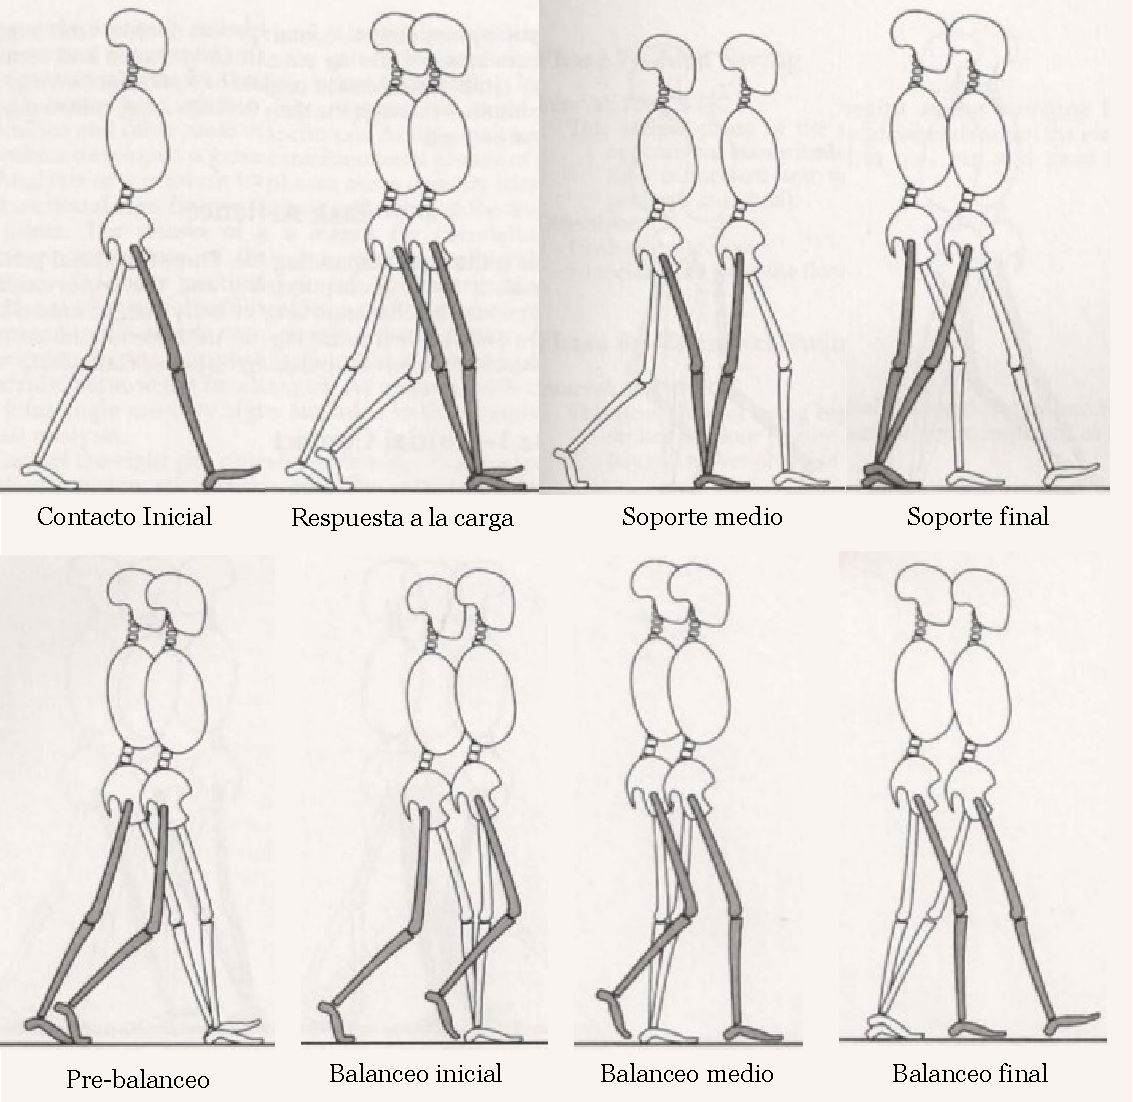
\includegraphics[height=0.7\textheight]{../report/imagenes/ciclo_marcha}
        \caption{Ilustración del ciclo de la marcha, tomado de \citep{perry}}
    \end{figure}
\end{frame}


\begin{frame}{Definiciones}
    \emph{Desarrollo de un software framework para el análisis de variables cinemáticas y espacio-temporales de la marcha.} \\
    \begin{block}{Software framework}
        Conjunto de funciones en un flujo de trabajo que proveen una funcionalidad genérica. 
    \end{block}
    \begin{block}{Variable cinemática}
        Cantidad relacionada con la posición, velocidad o aceleración de una unión del cuerpo.
    \end{block}
    \begin{block}{Variable espacio-temporal}
        Cantidad que expresa de manera global el movimiento del cuerpo.
    \end{block}
\end{frame}

%================================================================
\section{Solución propuesta}

\begin{frame}{Solución propuesta}
    \begin{block}{}
        Se desarrollaron contenedores genéricos para soportar los algoritmos, con un api muy semejante a STL++, para facilitar eventualmente hacer un \emph{port}.
    \end{block}
\end{frame}

\begin{frame}{Carga de datos}
\begin{table}
    \centering
    \caption{Funciones relacionadas a archivos bvh}
    \label{tab:bvh}
    \scriptsize 
    \begin{tabular}{ll}
        \toprule
        Nombre & Descripción \\
        \midrule
        \mono{bvh\_load\_data} & Carga un archivo BVH a un objeto \mono{motion}. \\
        \mono{bvh\_load\_directory} & Interpreta todos los archivos de un directorio como formato \\ & BVH y los carga en un vector \mono{motion\_vector}. \\
        \mono{bvh\_unload\_data} & Destruye un objeto \mono{motion} y libera la memoria. \\
        \mono{bvh\_unload\_directory} & Destruye un objeto \mono{motion\_vector}, incluyendo su contenido, \\ & y libera memoria. \\
        \bottomrule
    \end{tabular}
\end{table}
\end{frame}

\begin{frame}{Variables cinemáticas}
\begin{table}
    \centering
    \caption{Funciones sobre variables cinemáticas}
    \label{tab:kinematics}
    \scriptsize
    \begin{tabular}{ll}
        \toprule
        Nombre & Descripción \\
        \midrule
        \mono{derivate} & Deriva un \mono{time\_series}. \\
        \mono{integrate} & Integra un \mono{time\_series}. \\
        \mono{std\_planes\_calculate} & Calcula los planes de simetría estándar. \\
        \mono{transform\_egocentric} & Transforma todos los puntos al sistema egocéntrico \\ & definido por los planos estándar. \\
        \mono{vector\_vector} & Calcula un vector entre dos puntos. \\
        \mono{vector\_cross\_product} & Calcula el producto cruz de dos vectores. \\
        \mono{vector\_dot\_product} & Calcula el producto punto de dos vectores. \\
        \mono{vector\_normalize} & Normaliza a un vector unitario. \\
        \mono{vector\_project\_plane} & Proyecta un vector sobre un plano. \\
        \mono{vector\_calculate\_angle} & Calcula el ángulo entre dos vectores, opcionalmente \\ & los proyecta primero sobre un plano. \\
        \bottomrule
    \end{tabular}
\end{table}
\end{frame}

\begin{frame}{Variables espacio-temporales}
\begin{table}
    \centering
    \caption{Funciones sobre variables espacio-temporales}
    \label{tab:space-tmp}
    \scriptsize
    \begin{tabular}{ll}
        \toprule
        Nombre & Descripción \\
        \midrule
        \mono{linear\_fit} & Calcula una recta de tendencia de la forma $y = mx + b$. \\
        \mono{detect\_peaks} & Identifica los valles en una señal unidimensional. \\
        \mono{detect\_steps} & Identifica los pasos en un componente de un time-series. \\
        \mono{cadence} & Calcula la cadencia. \\
        \mono{distance} & Calcula la distancia tridimensional recorrida. \\
        \mono{step\_length} & Calcula la distancia de cada paso. \\
        \mono{step\_time} & Calcula la duración de cada paso. \\
        \bottomrule
    \end{tabular}
\end{table}
\end{frame}

\begin{frame}{Técnicas de análisis}
\begin{table}
    \centering
    \caption{Funciones para analizar las variables}
    \label{tab:analytics}
    \scriptsize
    \begin{tabular}{ll}
        \toprule
        Nombre & Descripción \\
        \midrule
        \mono{calc\_mean\_std\_dev} & Calcula la media y desviación estándar de un vector de valores reales. \\
        \mono{rms\_error} & Calcula el valor RMS de una señal o el error RMS entre dos señales. \\
        \mono{gait\_ration} & Razón de la longitud media del paso entre la cadencia. \\
        \mono{fourier\_transform} & Calcula la transformada de Fourier. \\
        \mono{armonic\_ratio} & Calcula la razón armónica de la marcha. \\
        \mono{t\_test\_one\_sample} & Calcula la significancia de que la media de una secuencia de valores \\ &  sea un valor en particular. \\
        \mono{t\_test\_two\_samples} & Calcula que la significancia de que media de dos secuencias de \\ & valores sea igual. \\
        \mono{t\_test\_Welcth} & Igual a la anterior pero sin asumir que la secuencia tiene la misma \\ & desviación estándar. \\
        \mono{anova\_one\_way} & Calcula el impacto de un factor sobre varios niveles. \\
        \bottomrule
    \end{tabular}
\end{table}
\end{frame}

%================================================================
\section{Algoritmo de detección de pasos}

\begin{frame}{Algoritmo de detección de pasos}
    % GNUPLOT: LaTeX picture
\setlength{\unitlength}{0.240900pt}
\ifx\plotpoint\undefined\newsavebox{\plotpoint}\fi
\begin{picture}(1500,900)(0,0)
\sbox{\plotpoint}{\rule[-0.200pt]{0.400pt}{0.400pt}}%
\put(191.0,131.0){\rule[-0.200pt]{4.818pt}{0.400pt}}
\put(171,131){\makebox(0,0)[r]{ 0.05}}
\put(1419.0,131.0){\rule[-0.200pt]{4.818pt}{0.400pt}}
\put(191.0,239.0){\rule[-0.200pt]{4.818pt}{0.400pt}}
\put(171,239){\makebox(0,0)[r]{ 0.1}}
\put(1419.0,239.0){\rule[-0.200pt]{4.818pt}{0.400pt}}
\put(191.0,346.0){\rule[-0.200pt]{4.818pt}{0.400pt}}
\put(171,346){\makebox(0,0)[r]{ 0.15}}
\put(1419.0,346.0){\rule[-0.200pt]{4.818pt}{0.400pt}}
\put(191.0,454.0){\rule[-0.200pt]{4.818pt}{0.400pt}}
\put(171,454){\makebox(0,0)[r]{ 0.2}}
\put(1419.0,454.0){\rule[-0.200pt]{4.818pt}{0.400pt}}
\put(191.0,561.0){\rule[-0.200pt]{4.818pt}{0.400pt}}
\put(171,561){\makebox(0,0)[r]{ 0.25}}
\put(1419.0,561.0){\rule[-0.200pt]{4.818pt}{0.400pt}}
\put(191.0,669.0){\rule[-0.200pt]{4.818pt}{0.400pt}}
\put(171,669){\makebox(0,0)[r]{ 0.3}}
\put(1419.0,669.0){\rule[-0.200pt]{4.818pt}{0.400pt}}
\put(191.0,776.0){\rule[-0.200pt]{4.818pt}{0.400pt}}
\put(171,776){\makebox(0,0)[r]{ 0.35}}
\put(1419.0,776.0){\rule[-0.200pt]{4.818pt}{0.400pt}}
\put(333.0,131.0){\rule[-0.200pt]{0.400pt}{4.818pt}}
\put(333,90){\makebox(0,0){ 400}}
\put(333.0,756.0){\rule[-0.200pt]{0.400pt}{4.818pt}}
\put(542.0,131.0){\rule[-0.200pt]{0.400pt}{4.818pt}}
\put(542,90){\makebox(0,0){ 600}}
\put(542.0,756.0){\rule[-0.200pt]{0.400pt}{4.818pt}}
\put(752.0,131.0){\rule[-0.200pt]{0.400pt}{4.818pt}}
\put(752,90){\makebox(0,0){ 800}}
\put(752.0,756.0){\rule[-0.200pt]{0.400pt}{4.818pt}}
\put(962.0,131.0){\rule[-0.200pt]{0.400pt}{4.818pt}}
\put(962,90){\makebox(0,0){ 1000}}
\put(962.0,756.0){\rule[-0.200pt]{0.400pt}{4.818pt}}
\put(1172.0,131.0){\rule[-0.200pt]{0.400pt}{4.818pt}}
\put(1172,90){\makebox(0,0){ 1200}}
\put(1172.0,756.0){\rule[-0.200pt]{0.400pt}{4.818pt}}
\put(1381.0,131.0){\rule[-0.200pt]{0.400pt}{4.818pt}}
\put(1381,90){\makebox(0,0){ 1400}}
\put(1381.0,756.0){\rule[-0.200pt]{0.400pt}{4.818pt}}
\put(191.0,131.0){\rule[-0.200pt]{0.400pt}{155.380pt}}
\put(191.0,131.0){\rule[-0.200pt]{300.643pt}{0.400pt}}
\put(1439.0,131.0){\rule[-0.200pt]{0.400pt}{155.380pt}}
\put(191.0,776.0){\rule[-0.200pt]{300.643pt}{0.400pt}}
\put(30,453){\makebox(0,0){\rotatebox{90}{Altura (m)}}}
\put(815,29){\makebox(0,0){Frames}}
\put(815,838){\makebox(0,0){Altura del talon}}
\put(191,237){\rule{1pt}{1pt}}
\put(192,237){\rule{1pt}{1pt}}
\put(193,236){\rule{1pt}{1pt}}
\put(194,236){\rule{1pt}{1pt}}
\put(195,235){\rule{1pt}{1pt}}
\put(196,234){\rule{1pt}{1pt}}
\put(197,234){\rule{1pt}{1pt}}
\put(198,233){\rule{1pt}{1pt}}
\put(199,233){\rule{1pt}{1pt}}
\put(200,233){\rule{1pt}{1pt}}
\put(201,233){\rule{1pt}{1pt}}
\put(203,233){\rule{1pt}{1pt}}
\put(204,233){\rule{1pt}{1pt}}
\put(205,234){\rule{1pt}{1pt}}
\put(206,234){\rule{1pt}{1pt}}
\put(207,234){\rule{1pt}{1pt}}
\put(208,235){\rule{1pt}{1pt}}
\put(209,235){\rule{1pt}{1pt}}
\put(210,235){\rule{1pt}{1pt}}
\put(211,236){\rule{1pt}{1pt}}
\put(212,236){\rule{1pt}{1pt}}
\put(213,237){\rule{1pt}{1pt}}
\put(214,237){\rule{1pt}{1pt}}
\put(215,238){\rule{1pt}{1pt}}
\put(216,238){\rule{1pt}{1pt}}
\put(217,239){\rule{1pt}{1pt}}
\put(218,239){\rule{1pt}{1pt}}
\put(219,240){\rule{1pt}{1pt}}
\put(220,240){\rule{1pt}{1pt}}
\put(221,241){\rule{1pt}{1pt}}
\put(222,241){\rule{1pt}{1pt}}
\put(224,242){\rule{1pt}{1pt}}
\put(225,241){\rule{1pt}{1pt}}
\put(226,242){\rule{1pt}{1pt}}
\put(227,242){\rule{1pt}{1pt}}
\put(228,242){\rule{1pt}{1pt}}
\put(229,242){\rule{1pt}{1pt}}
\put(230,242){\rule{1pt}{1pt}}
\put(231,243){\rule{1pt}{1pt}}
\put(232,243){\rule{1pt}{1pt}}
\put(233,243){\rule{1pt}{1pt}}
\put(234,242){\rule{1pt}{1pt}}
\put(235,243){\rule{1pt}{1pt}}
\put(236,243){\rule{1pt}{1pt}}
\put(237,244){\rule{1pt}{1pt}}
\put(238,244){\rule{1pt}{1pt}}
\put(239,244){\rule{1pt}{1pt}}
\put(240,244){\rule{1pt}{1pt}}
\put(241,244){\rule{1pt}{1pt}}
\put(242,245){\rule{1pt}{1pt}}
\put(243,245){\rule{1pt}{1pt}}
\put(244,246){\rule{1pt}{1pt}}
\put(246,247){\rule{1pt}{1pt}}
\put(247,245){\rule{1pt}{1pt}}
\put(248,247){\rule{1pt}{1pt}}
\put(249,249){\rule{1pt}{1pt}}
\put(250,248){\rule{1pt}{1pt}}
\put(251,251){\rule{1pt}{1pt}}
\put(252,248){\rule{1pt}{1pt}}
\put(253,249){\rule{1pt}{1pt}}
\put(254,249){\rule{1pt}{1pt}}
\put(255,244){\rule{1pt}{1pt}}
\put(256,250){\rule{1pt}{1pt}}
\put(257,250){\rule{1pt}{1pt}}
\put(258,248){\rule{1pt}{1pt}}
\put(259,249){\rule{1pt}{1pt}}
\put(260,249){\rule{1pt}{1pt}}
\put(261,256){\rule{1pt}{1pt}}
\put(262,253){\rule{1pt}{1pt}}
\put(263,249){\rule{1pt}{1pt}}
\put(264,252){\rule{1pt}{1pt}}
\put(265,252){\rule{1pt}{1pt}}
\put(267,253){\rule{1pt}{1pt}}
\put(268,253){\rule{1pt}{1pt}}
\put(269,254){\rule{1pt}{1pt}}
\put(270,255){\rule{1pt}{1pt}}
\put(271,257){\rule{1pt}{1pt}}
\put(272,258){\rule{1pt}{1pt}}
\put(273,259){\rule{1pt}{1pt}}
\put(274,260){\rule{1pt}{1pt}}
\put(275,262){\rule{1pt}{1pt}}
\put(276,264){\rule{1pt}{1pt}}
\put(277,266){\rule{1pt}{1pt}}
\put(278,268){\rule{1pt}{1pt}}
\put(279,270){\rule{1pt}{1pt}}
\put(280,273){\rule{1pt}{1pt}}
\put(281,276){\rule{1pt}{1pt}}
\put(282,278){\rule{1pt}{1pt}}
\put(283,281){\rule{1pt}{1pt}}
\put(284,285){\rule{1pt}{1pt}}
\put(285,288){\rule{1pt}{1pt}}
\put(286,292){\rule{1pt}{1pt}}
\put(287,296){\rule{1pt}{1pt}}
\put(289,300){\rule{1pt}{1pt}}
\put(290,304){\rule{1pt}{1pt}}
\put(291,308){\rule{1pt}{1pt}}
\put(292,313){\rule{1pt}{1pt}}
\put(293,318){\rule{1pt}{1pt}}
\put(294,324){\rule{1pt}{1pt}}
\put(295,329){\rule{1pt}{1pt}}
\put(296,335){\rule{1pt}{1pt}}
\put(297,341){\rule{1pt}{1pt}}
\put(298,347){\rule{1pt}{1pt}}
\put(299,353){\rule{1pt}{1pt}}
\put(300,359){\rule{1pt}{1pt}}
\put(301,365){\rule{1pt}{1pt}}
\put(302,372){\rule{1pt}{1pt}}
\put(303,379){\rule{1pt}{1pt}}
\put(304,385){\rule{1pt}{1pt}}
\put(305,392){\rule{1pt}{1pt}}
\put(306,399){\rule{1pt}{1pt}}
\put(307,406){\rule{1pt}{1pt}}
\put(308,413){\rule{1pt}{1pt}}
\put(310,420){\rule{1pt}{1pt}}
\put(311,427){\rule{1pt}{1pt}}
\put(312,434){\rule{1pt}{1pt}}
\put(313,442){\rule{1pt}{1pt}}
\put(314,449){\rule{1pt}{1pt}}
\put(315,457){\rule{1pt}{1pt}}
\put(316,465){\rule{1pt}{1pt}}
\put(317,473){\rule{1pt}{1pt}}
\put(318,481){\rule{1pt}{1pt}}
\put(319,490){\rule{1pt}{1pt}}
\put(320,499){\rule{1pt}{1pt}}
\put(321,508){\rule{1pt}{1pt}}
\put(322,517){\rule{1pt}{1pt}}
\put(323,525){\rule{1pt}{1pt}}
\put(324,533){\rule{1pt}{1pt}}
\put(325,541){\rule{1pt}{1pt}}
\put(326,551){\rule{1pt}{1pt}}
\put(327,560){\rule{1pt}{1pt}}
\put(328,568){\rule{1pt}{1pt}}
\put(329,575){\rule{1pt}{1pt}}
\put(330,583){\rule{1pt}{1pt}}
\put(332,590){\rule{1pt}{1pt}}
\put(333,596){\rule{1pt}{1pt}}
\put(334,602){\rule{1pt}{1pt}}
\put(335,608){\rule{1pt}{1pt}}
\put(336,612){\rule{1pt}{1pt}}
\put(337,615){\rule{1pt}{1pt}}
\put(338,618){\rule{1pt}{1pt}}
\put(339,619){\rule{1pt}{1pt}}
\put(340,620){\rule{1pt}{1pt}}
\put(341,620){\rule{1pt}{1pt}}
\put(342,619){\rule{1pt}{1pt}}
\put(343,618){\rule{1pt}{1pt}}
\put(344,616){\rule{1pt}{1pt}}
\put(345,613){\rule{1pt}{1pt}}
\put(346,610){\rule{1pt}{1pt}}
\put(347,606){\rule{1pt}{1pt}}
\put(348,601){\rule{1pt}{1pt}}
\put(349,596){\rule{1pt}{1pt}}
\put(350,589){\rule{1pt}{1pt}}
\put(351,583){\rule{1pt}{1pt}}
\put(353,576){\rule{1pt}{1pt}}
\put(354,569){\rule{1pt}{1pt}}
\put(355,561){\rule{1pt}{1pt}}
\put(356,553){\rule{1pt}{1pt}}
\put(357,545){\rule{1pt}{1pt}}
\put(358,536){\rule{1pt}{1pt}}
\put(359,528){\rule{1pt}{1pt}}
\put(360,519){\rule{1pt}{1pt}}
\put(361,511){\rule{1pt}{1pt}}
\put(362,502){\rule{1pt}{1pt}}
\put(363,493){\rule{1pt}{1pt}}
\put(364,484){\rule{1pt}{1pt}}
\put(365,474){\rule{1pt}{1pt}}
\put(366,464){\rule{1pt}{1pt}}
\put(367,455){\rule{1pt}{1pt}}
\put(368,446){\rule{1pt}{1pt}}
\put(369,436){\rule{1pt}{1pt}}
\put(370,427){\rule{1pt}{1pt}}
\put(371,418){\rule{1pt}{1pt}}
\put(372,409){\rule{1pt}{1pt}}
\put(373,401){\rule{1pt}{1pt}}
\put(375,392){\rule{1pt}{1pt}}
\put(376,384){\rule{1pt}{1pt}}
\put(377,376){\rule{1pt}{1pt}}
\put(378,368){\rule{1pt}{1pt}}
\put(379,360){\rule{1pt}{1pt}}
\put(380,352){\rule{1pt}{1pt}}
\put(381,345){\rule{1pt}{1pt}}
\put(382,339){\rule{1pt}{1pt}}
\put(383,332){\rule{1pt}{1pt}}
\put(384,325){\rule{1pt}{1pt}}
\put(385,319){\rule{1pt}{1pt}}
\put(386,313){\rule{1pt}{1pt}}
\put(387,308){\rule{1pt}{1pt}}
\put(388,303){\rule{1pt}{1pt}}
\put(389,299){\rule{1pt}{1pt}}
\put(390,294){\rule{1pt}{1pt}}
\put(391,290){\rule{1pt}{1pt}}
\put(392,287){\rule{1pt}{1pt}}
\put(393,284){\rule{1pt}{1pt}}
\put(394,281){\rule{1pt}{1pt}}
\put(396,279){\rule{1pt}{1pt}}
\put(397,277){\rule{1pt}{1pt}}
\put(398,275){\rule{1pt}{1pt}}
\put(399,273){\rule{1pt}{1pt}}
\put(400,273){\rule{1pt}{1pt}}
\put(401,272){\rule{1pt}{1pt}}
\put(402,272){\rule{1pt}{1pt}}
\put(403,272){\rule{1pt}{1pt}}
\put(404,272){\rule{1pt}{1pt}}
\put(405,273){\rule{1pt}{1pt}}
\put(406,274){\rule{1pt}{1pt}}
\put(407,275){\rule{1pt}{1pt}}
\put(408,277){\rule{1pt}{1pt}}
\put(409,278){\rule{1pt}{1pt}}
\put(410,280){\rule{1pt}{1pt}}
\put(411,282){\rule{1pt}{1pt}}
\put(412,284){\rule{1pt}{1pt}}
\put(413,286){\rule{1pt}{1pt}}
\put(414,288){\rule{1pt}{1pt}}
\put(415,289){\rule{1pt}{1pt}}
\put(416,291){\rule{1pt}{1pt}}
\put(418,292){\rule{1pt}{1pt}}
\put(419,293){\rule{1pt}{1pt}}
\put(420,294){\rule{1pt}{1pt}}
\put(421,294){\rule{1pt}{1pt}}
\put(422,293){\rule{1pt}{1pt}}
\put(423,293){\rule{1pt}{1pt}}
\put(424,291){\rule{1pt}{1pt}}
\put(425,290){\rule{1pt}{1pt}}
\put(426,288){\rule{1pt}{1pt}}
\put(427,285){\rule{1pt}{1pt}}
\put(428,282){\rule{1pt}{1pt}}
\put(429,279){\rule{1pt}{1pt}}
\put(430,276){\rule{1pt}{1pt}}
\put(431,272){\rule{1pt}{1pt}}
\put(432,268){\rule{1pt}{1pt}}
\put(433,264){\rule{1pt}{1pt}}
\put(434,260){\rule{1pt}{1pt}}
\put(435,255){\rule{1pt}{1pt}}
\put(436,251){\rule{1pt}{1pt}}
\put(437,248){\rule{1pt}{1pt}}
\put(439,245){\rule{1pt}{1pt}}
\put(440,242){\rule{1pt}{1pt}}
\put(441,240){\rule{1pt}{1pt}}
\put(442,237){\rule{1pt}{1pt}}
\put(443,235){\rule{1pt}{1pt}}
\put(444,232){\rule{1pt}{1pt}}
\put(445,231){\rule{1pt}{1pt}}
\put(446,229){\rule{1pt}{1pt}}
\put(447,227){\rule{1pt}{1pt}}
\put(448,226){\rule{1pt}{1pt}}
\put(449,225){\rule{1pt}{1pt}}
\put(450,224){\rule{1pt}{1pt}}
\put(451,223){\rule{1pt}{1pt}}
\put(452,222){\rule{1pt}{1pt}}
\put(453,222){\rule{1pt}{1pt}}
\put(454,222){\rule{1pt}{1pt}}
\put(455,222){\rule{1pt}{1pt}}
\put(456,222){\rule{1pt}{1pt}}
\put(457,222){\rule{1pt}{1pt}}
\put(458,222){\rule{1pt}{1pt}}
\put(459,222){\rule{1pt}{1pt}}
\put(461,222){\rule{1pt}{1pt}}
\put(462,222){\rule{1pt}{1pt}}
\put(463,222){\rule{1pt}{1pt}}
\put(464,222){\rule{1pt}{1pt}}
\put(465,222){\rule{1pt}{1pt}}
\put(466,222){\rule{1pt}{1pt}}
\put(467,222){\rule{1pt}{1pt}}
\put(468,222){\rule{1pt}{1pt}}
\put(469,222){\rule{1pt}{1pt}}
\put(470,221){\rule{1pt}{1pt}}
\put(471,221){\rule{1pt}{1pt}}
\put(472,221){\rule{1pt}{1pt}}
\put(473,222){\rule{1pt}{1pt}}
\put(474,221){\rule{1pt}{1pt}}
\put(475,222){\rule{1pt}{1pt}}
\put(476,222){\rule{1pt}{1pt}}
\put(477,222){\rule{1pt}{1pt}}
\put(478,223){\rule{1pt}{1pt}}
\put(479,223){\rule{1pt}{1pt}}
\put(480,224){\rule{1pt}{1pt}}
\put(482,224){\rule{1pt}{1pt}}
\put(483,225){\rule{1pt}{1pt}}
\put(484,226){\rule{1pt}{1pt}}
\put(485,227){\rule{1pt}{1pt}}
\put(486,227){\rule{1pt}{1pt}}
\put(487,228){\rule{1pt}{1pt}}
\put(488,229){\rule{1pt}{1pt}}
\put(489,230){\rule{1pt}{1pt}}
\put(490,231){\rule{1pt}{1pt}}
\put(491,232){\rule{1pt}{1pt}}
\put(492,233){\rule{1pt}{1pt}}
\put(493,234){\rule{1pt}{1pt}}
\put(494,234){\rule{1pt}{1pt}}
\put(495,235){\rule{1pt}{1pt}}
\put(496,236){\rule{1pt}{1pt}}
\put(497,237){\rule{1pt}{1pt}}
\put(498,238){\rule{1pt}{1pt}}
\put(499,239){\rule{1pt}{1pt}}
\put(500,239){\rule{1pt}{1pt}}
\put(501,240){\rule{1pt}{1pt}}
\put(502,241){\rule{1pt}{1pt}}
\put(504,241){\rule{1pt}{1pt}}
\put(505,242){\rule{1pt}{1pt}}
\put(506,243){\rule{1pt}{1pt}}
\put(507,243){\rule{1pt}{1pt}}
\put(508,244){\rule{1pt}{1pt}}
\put(509,245){\rule{1pt}{1pt}}
\put(510,245){\rule{1pt}{1pt}}
\put(511,246){\rule{1pt}{1pt}}
\put(512,247){\rule{1pt}{1pt}}
\put(513,247){\rule{1pt}{1pt}}
\put(514,248){\rule{1pt}{1pt}}
\put(515,248){\rule{1pt}{1pt}}
\put(516,249){\rule{1pt}{1pt}}
\put(517,249){\rule{1pt}{1pt}}
\put(518,250){\rule{1pt}{1pt}}
\put(519,250){\rule{1pt}{1pt}}
\put(520,251){\rule{1pt}{1pt}}
\put(521,251){\rule{1pt}{1pt}}
\put(522,252){\rule{1pt}{1pt}}
\put(523,252){\rule{1pt}{1pt}}
\put(524,253){\rule{1pt}{1pt}}
\put(526,253){\rule{1pt}{1pt}}
\put(527,253){\rule{1pt}{1pt}}
\put(528,254){\rule{1pt}{1pt}}
\put(529,255){\rule{1pt}{1pt}}
\put(530,255){\rule{1pt}{1pt}}
\put(531,256){\rule{1pt}{1pt}}
\put(532,257){\rule{1pt}{1pt}}
\put(533,257){\rule{1pt}{1pt}}
\put(534,258){\rule{1pt}{1pt}}
\put(535,259){\rule{1pt}{1pt}}
\put(536,261){\rule{1pt}{1pt}}
\put(537,262){\rule{1pt}{1pt}}
\put(538,264){\rule{1pt}{1pt}}
\put(539,265){\rule{1pt}{1pt}}
\put(540,268){\rule{1pt}{1pt}}
\put(541,270){\rule{1pt}{1pt}}
\put(542,273){\rule{1pt}{1pt}}
\put(543,276){\rule{1pt}{1pt}}
\put(544,279){\rule{1pt}{1pt}}
\put(545,282){\rule{1pt}{1pt}}
\put(547,286){\rule{1pt}{1pt}}
\put(548,290){\rule{1pt}{1pt}}
\put(549,295){\rule{1pt}{1pt}}
\put(550,299){\rule{1pt}{1pt}}
\put(551,305){\rule{1pt}{1pt}}
\put(552,310){\rule{1pt}{1pt}}
\put(553,316){\rule{1pt}{1pt}}
\put(554,322){\rule{1pt}{1pt}}
\put(555,328){\rule{1pt}{1pt}}
\put(556,334){\rule{1pt}{1pt}}
\put(557,341){\rule{1pt}{1pt}}
\put(558,348){\rule{1pt}{1pt}}
\put(559,355){\rule{1pt}{1pt}}
\put(560,362){\rule{1pt}{1pt}}
\put(561,369){\rule{1pt}{1pt}}
\put(562,377){\rule{1pt}{1pt}}
\put(563,384){\rule{1pt}{1pt}}
\put(564,392){\rule{1pt}{1pt}}
\put(565,400){\rule{1pt}{1pt}}
\put(566,408){\rule{1pt}{1pt}}
\put(567,416){\rule{1pt}{1pt}}
\put(569,424){\rule{1pt}{1pt}}
\put(570,432){\rule{1pt}{1pt}}
\put(571,440){\rule{1pt}{1pt}}
\put(572,448){\rule{1pt}{1pt}}
\put(573,456){\rule{1pt}{1pt}}
\put(574,464){\rule{1pt}{1pt}}
\put(575,473){\rule{1pt}{1pt}}
\put(576,481){\rule{1pt}{1pt}}
\put(577,490){\rule{1pt}{1pt}}
\put(578,500){\rule{1pt}{1pt}}
\put(579,510){\rule{1pt}{1pt}}
\put(580,520){\rule{1pt}{1pt}}
\put(581,530){\rule{1pt}{1pt}}
\put(582,540){\rule{1pt}{1pt}}
\put(583,548){\rule{1pt}{1pt}}
\put(584,558){\rule{1pt}{1pt}}
\put(585,568){\rule{1pt}{1pt}}
\put(586,577){\rule{1pt}{1pt}}
\put(587,586){\rule{1pt}{1pt}}
\put(588,595){\rule{1pt}{1pt}}
\put(590,604){\rule{1pt}{1pt}}
\put(591,613){\rule{1pt}{1pt}}
\put(592,622){\rule{1pt}{1pt}}
\put(593,630){\rule{1pt}{1pt}}
\put(594,638){\rule{1pt}{1pt}}
\put(595,645){\rule{1pt}{1pt}}
\put(596,651){\rule{1pt}{1pt}}
\put(597,656){\rule{1pt}{1pt}}
\put(598,660){\rule{1pt}{1pt}}
\put(599,664){\rule{1pt}{1pt}}
\put(600,667){\rule{1pt}{1pt}}
\put(601,669){\rule{1pt}{1pt}}
\put(602,670){\rule{1pt}{1pt}}
\put(603,671){\rule{1pt}{1pt}}
\put(604,671){\rule{1pt}{1pt}}
\put(605,670){\rule{1pt}{1pt}}
\put(606,669){\rule{1pt}{1pt}}
\put(607,667){\rule{1pt}{1pt}}
\put(608,665){\rule{1pt}{1pt}}
\put(609,661){\rule{1pt}{1pt}}
\put(610,657){\rule{1pt}{1pt}}
\put(612,653){\rule{1pt}{1pt}}
\put(613,648){\rule{1pt}{1pt}}
\put(614,643){\rule{1pt}{1pt}}
\put(615,637){\rule{1pt}{1pt}}
\put(616,630){\rule{1pt}{1pt}}
\put(617,623){\rule{1pt}{1pt}}
\put(618,616){\rule{1pt}{1pt}}
\put(619,608){\rule{1pt}{1pt}}
\put(620,599){\rule{1pt}{1pt}}
\put(621,591){\rule{1pt}{1pt}}
\put(622,581){\rule{1pt}{1pt}}
\put(623,572){\rule{1pt}{1pt}}
\put(624,563){\rule{1pt}{1pt}}
\put(625,554){\rule{1pt}{1pt}}
\put(626,544){\rule{1pt}{1pt}}
\put(627,534){\rule{1pt}{1pt}}
\put(628,525){\rule{1pt}{1pt}}
\put(629,515){\rule{1pt}{1pt}}
\put(630,505){\rule{1pt}{1pt}}
\put(631,495){\rule{1pt}{1pt}}
\put(633,485){\rule{1pt}{1pt}}
\put(634,474){\rule{1pt}{1pt}}
\put(635,464){\rule{1pt}{1pt}}
\put(636,454){\rule{1pt}{1pt}}
\put(637,443){\rule{1pt}{1pt}}
\put(638,433){\rule{1pt}{1pt}}
\put(639,423){\rule{1pt}{1pt}}
\put(640,413){\rule{1pt}{1pt}}
\put(641,403){\rule{1pt}{1pt}}
\put(642,394){\rule{1pt}{1pt}}
\put(643,384){\rule{1pt}{1pt}}
\put(644,375){\rule{1pt}{1pt}}
\put(645,366){\rule{1pt}{1pt}}
\put(646,357){\rule{1pt}{1pt}}
\put(647,348){\rule{1pt}{1pt}}
\put(648,340){\rule{1pt}{1pt}}
\put(649,331){\rule{1pt}{1pt}}
\put(650,324){\rule{1pt}{1pt}}
\put(651,317){\rule{1pt}{1pt}}
\put(652,310){\rule{1pt}{1pt}}
\put(653,304){\rule{1pt}{1pt}}
\put(655,297){\rule{1pt}{1pt}}
\put(656,292){\rule{1pt}{1pt}}
\put(657,287){\rule{1pt}{1pt}}
\put(658,282){\rule{1pt}{1pt}}
\put(659,279){\rule{1pt}{1pt}}
\put(660,276){\rule{1pt}{1pt}}
\put(661,273){\rule{1pt}{1pt}}
\put(662,271){\rule{1pt}{1pt}}
\put(663,269){\rule{1pt}{1pt}}
\put(664,268){\rule{1pt}{1pt}}
\put(665,268){\rule{1pt}{1pt}}
\put(666,268){\rule{1pt}{1pt}}
\put(667,269){\rule{1pt}{1pt}}
\put(668,270){\rule{1pt}{1pt}}
\put(669,272){\rule{1pt}{1pt}}
\put(670,274){\rule{1pt}{1pt}}
\put(671,276){\rule{1pt}{1pt}}
\put(672,279){\rule{1pt}{1pt}}
\put(673,282){\rule{1pt}{1pt}}
\put(674,285){\rule{1pt}{1pt}}
\put(676,287){\rule{1pt}{1pt}}
\put(677,290){\rule{1pt}{1pt}}
\put(678,292){\rule{1pt}{1pt}}
\put(679,294){\rule{1pt}{1pt}}
\put(680,295){\rule{1pt}{1pt}}
\put(681,295){\rule{1pt}{1pt}}
\put(682,294){\rule{1pt}{1pt}}
\put(683,293){\rule{1pt}{1pt}}
\put(684,291){\rule{1pt}{1pt}}
\put(685,288){\rule{1pt}{1pt}}
\put(686,284){\rule{1pt}{1pt}}
\put(687,280){\rule{1pt}{1pt}}
\put(688,276){\rule{1pt}{1pt}}
\put(689,271){\rule{1pt}{1pt}}
\put(690,266){\rule{1pt}{1pt}}
\put(691,261){\rule{1pt}{1pt}}
\put(692,256){\rule{1pt}{1pt}}
\put(693,251){\rule{1pt}{1pt}}
\put(694,245){\rule{1pt}{1pt}}
\put(695,241){\rule{1pt}{1pt}}
\put(696,236){\rule{1pt}{1pt}}
\put(698,233){\rule{1pt}{1pt}}
\put(699,229){\rule{1pt}{1pt}}
\put(700,227){\rule{1pt}{1pt}}
\put(701,224){\rule{1pt}{1pt}}
\put(702,220){\rule{1pt}{1pt}}
\put(703,217){\rule{1pt}{1pt}}
\put(704,214){\rule{1pt}{1pt}}
\put(705,213){\rule{1pt}{1pt}}
\put(706,211){\rule{1pt}{1pt}}
\put(707,209){\rule{1pt}{1pt}}
\put(708,208){\rule{1pt}{1pt}}
\put(709,209){\rule{1pt}{1pt}}
\put(710,209){\rule{1pt}{1pt}}
\put(711,209){\rule{1pt}{1pt}}
\put(712,209){\rule{1pt}{1pt}}
\put(713,210){\rule{1pt}{1pt}}
\put(714,210){\rule{1pt}{1pt}}
\put(715,210){\rule{1pt}{1pt}}
\put(716,210){\rule{1pt}{1pt}}
\put(717,210){\rule{1pt}{1pt}}
\put(719,210){\rule{1pt}{1pt}}
\put(720,210){\rule{1pt}{1pt}}
\put(721,210){\rule{1pt}{1pt}}
\put(722,209){\rule{1pt}{1pt}}
\put(723,209){\rule{1pt}{1pt}}
\put(724,209){\rule{1pt}{1pt}}
\put(725,209){\rule{1pt}{1pt}}
\put(726,209){\rule{1pt}{1pt}}
\put(727,209){\rule{1pt}{1pt}}
\put(728,209){\rule{1pt}{1pt}}
\put(729,209){\rule{1pt}{1pt}}
\put(730,209){\rule{1pt}{1pt}}
\put(731,210){\rule{1pt}{1pt}}
\put(732,210){\rule{1pt}{1pt}}
\put(733,211){\rule{1pt}{1pt}}
\put(734,211){\rule{1pt}{1pt}}
\put(735,212){\rule{1pt}{1pt}}
\put(736,213){\rule{1pt}{1pt}}
\put(737,213){\rule{1pt}{1pt}}
\put(738,214){\rule{1pt}{1pt}}
\put(739,215){\rule{1pt}{1pt}}
\put(741,216){\rule{1pt}{1pt}}
\put(742,216){\rule{1pt}{1pt}}
\put(743,217){\rule{1pt}{1pt}}
\put(744,217){\rule{1pt}{1pt}}
\put(745,218){\rule{1pt}{1pt}}
\put(746,219){\rule{1pt}{1pt}}
\put(747,220){\rule{1pt}{1pt}}
\put(748,221){\rule{1pt}{1pt}}
\put(749,222){\rule{1pt}{1pt}}
\put(750,223){\rule{1pt}{1pt}}
\put(751,224){\rule{1pt}{1pt}}
\put(752,226){\rule{1pt}{1pt}}
\put(753,227){\rule{1pt}{1pt}}
\put(754,228){\rule{1pt}{1pt}}
\put(755,229){\rule{1pt}{1pt}}
\put(756,230){\rule{1pt}{1pt}}
\put(757,231){\rule{1pt}{1pt}}
\put(758,232){\rule{1pt}{1pt}}
\put(759,233){\rule{1pt}{1pt}}
\put(760,234){\rule{1pt}{1pt}}
\put(762,236){\rule{1pt}{1pt}}
\put(763,237){\rule{1pt}{1pt}}
\put(764,238){\rule{1pt}{1pt}}
\put(765,239){\rule{1pt}{1pt}}
\put(766,240){\rule{1pt}{1pt}}
\put(767,241){\rule{1pt}{1pt}}
\put(768,242){\rule{1pt}{1pt}}
\put(769,243){\rule{1pt}{1pt}}
\put(770,244){\rule{1pt}{1pt}}
\put(771,244){\rule{1pt}{1pt}}
\put(772,245){\rule{1pt}{1pt}}
\put(773,246){\rule{1pt}{1pt}}
\put(774,247){\rule{1pt}{1pt}}
\put(775,247){\rule{1pt}{1pt}}
\put(776,248){\rule{1pt}{1pt}}
\put(777,248){\rule{1pt}{1pt}}
\put(778,249){\rule{1pt}{1pt}}
\put(779,249){\rule{1pt}{1pt}}
\put(780,250){\rule{1pt}{1pt}}
\put(781,250){\rule{1pt}{1pt}}
\put(782,251){\rule{1pt}{1pt}}
\put(784,252){\rule{1pt}{1pt}}
\put(785,252){\rule{1pt}{1pt}}
\put(786,253){\rule{1pt}{1pt}}
\put(787,253){\rule{1pt}{1pt}}
\put(788,254){\rule{1pt}{1pt}}
\put(789,255){\rule{1pt}{1pt}}
\put(790,256){\rule{1pt}{1pt}}
\put(791,257){\rule{1pt}{1pt}}
\put(792,259){\rule{1pt}{1pt}}
\put(793,260){\rule{1pt}{1pt}}
\put(794,262){\rule{1pt}{1pt}}
\put(795,264){\rule{1pt}{1pt}}
\put(796,266){\rule{1pt}{1pt}}
\put(797,268){\rule{1pt}{1pt}}
\put(798,270){\rule{1pt}{1pt}}
\put(799,273){\rule{1pt}{1pt}}
\put(800,276){\rule{1pt}{1pt}}
\put(801,279){\rule{1pt}{1pt}}
\put(802,283){\rule{1pt}{1pt}}
\put(803,286){\rule{1pt}{1pt}}
\put(805,291){\rule{1pt}{1pt}}
\put(806,296){\rule{1pt}{1pt}}
\put(807,300){\rule{1pt}{1pt}}
\put(808,306){\rule{1pt}{1pt}}
\put(809,311){\rule{1pt}{1pt}}
\put(810,317){\rule{1pt}{1pt}}
\put(811,323){\rule{1pt}{1pt}}
\put(812,329){\rule{1pt}{1pt}}
\put(813,335){\rule{1pt}{1pt}}
\put(814,342){\rule{1pt}{1pt}}
\put(815,349){\rule{1pt}{1pt}}
\put(816,356){\rule{1pt}{1pt}}
\put(817,364){\rule{1pt}{1pt}}
\put(818,372){\rule{1pt}{1pt}}
\put(819,379){\rule{1pt}{1pt}}
\put(820,387){\rule{1pt}{1pt}}
\put(821,395){\rule{1pt}{1pt}}
\put(822,403){\rule{1pt}{1pt}}
\put(823,410){\rule{1pt}{1pt}}
\put(824,418){\rule{1pt}{1pt}}
\put(825,426){\rule{1pt}{1pt}}
\put(827,434){\rule{1pt}{1pt}}
\put(828,442){\rule{1pt}{1pt}}
\put(829,450){\rule{1pt}{1pt}}
\put(830,458){\rule{1pt}{1pt}}
\put(831,466){\rule{1pt}{1pt}}
\put(832,475){\rule{1pt}{1pt}}
\put(833,484){\rule{1pt}{1pt}}
\put(834,492){\rule{1pt}{1pt}}
\put(835,501){\rule{1pt}{1pt}}
\put(836,510){\rule{1pt}{1pt}}
\put(837,519){\rule{1pt}{1pt}}
\put(838,527){\rule{1pt}{1pt}}
\put(839,535){\rule{1pt}{1pt}}
\put(840,546){\rule{1pt}{1pt}}
\put(841,554){\rule{1pt}{1pt}}
\put(842,563){\rule{1pt}{1pt}}
\put(843,571){\rule{1pt}{1pt}}
\put(844,579){\rule{1pt}{1pt}}
\put(845,586){\rule{1pt}{1pt}}
\put(846,594){\rule{1pt}{1pt}}
\put(848,602){\rule{1pt}{1pt}}
\put(849,609){\rule{1pt}{1pt}}
\put(850,615){\rule{1pt}{1pt}}
\put(851,621){\rule{1pt}{1pt}}
\put(852,626){\rule{1pt}{1pt}}
\put(853,630){\rule{1pt}{1pt}}
\put(854,633){\rule{1pt}{1pt}}
\put(855,636){\rule{1pt}{1pt}}
\put(856,638){\rule{1pt}{1pt}}
\put(857,639){\rule{1pt}{1pt}}
\put(858,640){\rule{1pt}{1pt}}
\put(859,640){\rule{1pt}{1pt}}
\put(860,640){\rule{1pt}{1pt}}
\put(861,639){\rule{1pt}{1pt}}
\put(862,637){\rule{1pt}{1pt}}
\put(863,635){\rule{1pt}{1pt}}
\put(864,631){\rule{1pt}{1pt}}
\put(865,628){\rule{1pt}{1pt}}
\put(866,623){\rule{1pt}{1pt}}
\put(867,619){\rule{1pt}{1pt}}
\put(868,613){\rule{1pt}{1pt}}
\put(870,608){\rule{1pt}{1pt}}
\put(871,602){\rule{1pt}{1pt}}
\put(872,595){\rule{1pt}{1pt}}
\put(873,588){\rule{1pt}{1pt}}
\put(874,580){\rule{1pt}{1pt}}
\put(875,573){\rule{1pt}{1pt}}
\put(876,564){\rule{1pt}{1pt}}
\put(877,556){\rule{1pt}{1pt}}
\put(878,546){\rule{1pt}{1pt}}
\put(879,537){\rule{1pt}{1pt}}
\put(880,529){\rule{1pt}{1pt}}
\put(881,519){\rule{1pt}{1pt}}
\put(882,510){\rule{1pt}{1pt}}
\put(883,501){\rule{1pt}{1pt}}
\put(884,492){\rule{1pt}{1pt}}
\put(885,482){\rule{1pt}{1pt}}
\put(886,473){\rule{1pt}{1pt}}
\put(887,464){\rule{1pt}{1pt}}
\put(888,454){\rule{1pt}{1pt}}
\put(889,445){\rule{1pt}{1pt}}
\put(891,435){\rule{1pt}{1pt}}
\put(892,426){\rule{1pt}{1pt}}
\put(893,417){\rule{1pt}{1pt}}
\put(894,407){\rule{1pt}{1pt}}
\put(895,398){\rule{1pt}{1pt}}
\put(896,389){\rule{1pt}{1pt}}
\put(897,380){\rule{1pt}{1pt}}
\put(898,372){\rule{1pt}{1pt}}
\put(899,363){\rule{1pt}{1pt}}
\put(900,355){\rule{1pt}{1pt}}
\put(901,347){\rule{1pt}{1pt}}
\put(902,340){\rule{1pt}{1pt}}
\put(903,332){\rule{1pt}{1pt}}
\put(904,325){\rule{1pt}{1pt}}
\put(905,319){\rule{1pt}{1pt}}
\put(906,312){\rule{1pt}{1pt}}
\put(907,306){\rule{1pt}{1pt}}
\put(908,301){\rule{1pt}{1pt}}
\put(909,295){\rule{1pt}{1pt}}
\put(910,291){\rule{1pt}{1pt}}
\put(911,287){\rule{1pt}{1pt}}
\put(913,283){\rule{1pt}{1pt}}
\put(914,280){\rule{1pt}{1pt}}
\put(915,277){\rule{1pt}{1pt}}
\put(916,275){\rule{1pt}{1pt}}
\put(917,273){\rule{1pt}{1pt}}
\put(918,272){\rule{1pt}{1pt}}
\put(919,271){\rule{1pt}{1pt}}
\put(920,271){\rule{1pt}{1pt}}
\put(921,272){\rule{1pt}{1pt}}
\put(922,272){\rule{1pt}{1pt}}
\put(923,274){\rule{1pt}{1pt}}
\put(924,275){\rule{1pt}{1pt}}
\put(925,277){\rule{1pt}{1pt}}
\put(926,280){\rule{1pt}{1pt}}
\put(927,283){\rule{1pt}{1pt}}
\put(928,285){\rule{1pt}{1pt}}
\put(929,289){\rule{1pt}{1pt}}
\put(930,292){\rule{1pt}{1pt}}
\put(931,295){\rule{1pt}{1pt}}
\put(932,298){\rule{1pt}{1pt}}
\put(934,301){\rule{1pt}{1pt}}
\put(935,304){\rule{1pt}{1pt}}
\put(936,307){\rule{1pt}{1pt}}
\put(937,309){\rule{1pt}{1pt}}
\put(938,310){\rule{1pt}{1pt}}
\put(939,311){\rule{1pt}{1pt}}
\put(940,311){\rule{1pt}{1pt}}
\put(941,311){\rule{1pt}{1pt}}
\put(942,310){\rule{1pt}{1pt}}
\put(943,308){\rule{1pt}{1pt}}
\put(944,306){\rule{1pt}{1pt}}
\put(945,303){\rule{1pt}{1pt}}
\put(946,299){\rule{1pt}{1pt}}
\put(947,295){\rule{1pt}{1pt}}
\put(948,291){\rule{1pt}{1pt}}
\put(949,286){\rule{1pt}{1pt}}
\put(950,281){\rule{1pt}{1pt}}
\put(951,276){\rule{1pt}{1pt}}
\put(952,270){\rule{1pt}{1pt}}
\put(953,265){\rule{1pt}{1pt}}
\put(954,259){\rule{1pt}{1pt}}
\put(956,253){\rule{1pt}{1pt}}
\put(957,248){\rule{1pt}{1pt}}
\put(958,243){\rule{1pt}{1pt}}
\put(959,238){\rule{1pt}{1pt}}
\put(960,234){\rule{1pt}{1pt}}
\put(961,230){\rule{1pt}{1pt}}
\put(962,226){\rule{1pt}{1pt}}
\put(963,222){\rule{1pt}{1pt}}
\put(964,218){\rule{1pt}{1pt}}
\put(965,214){\rule{1pt}{1pt}}
\put(966,210){\rule{1pt}{1pt}}
\put(967,208){\rule{1pt}{1pt}}
\put(968,206){\rule{1pt}{1pt}}
\put(969,205){\rule{1pt}{1pt}}
\put(970,204){\rule{1pt}{1pt}}
\put(971,203){\rule{1pt}{1pt}}
\put(972,203){\rule{1pt}{1pt}}
\put(973,203){\rule{1pt}{1pt}}
\put(974,204){\rule{1pt}{1pt}}
\put(975,204){\rule{1pt}{1pt}}
\put(977,205){\rule{1pt}{1pt}}
\put(978,205){\rule{1pt}{1pt}}
\put(979,205){\rule{1pt}{1pt}}
\put(980,205){\rule{1pt}{1pt}}
\put(981,206){\rule{1pt}{1pt}}
\put(982,206){\rule{1pt}{1pt}}
\put(983,206){\rule{1pt}{1pt}}
\put(984,206){\rule{1pt}{1pt}}
\put(985,206){\rule{1pt}{1pt}}
\put(986,206){\rule{1pt}{1pt}}
\put(987,206){\rule{1pt}{1pt}}
\put(988,206){\rule{1pt}{1pt}}
\put(989,205){\rule{1pt}{1pt}}
\put(990,205){\rule{1pt}{1pt}}
\put(991,206){\rule{1pt}{1pt}}
\put(992,206){\rule{1pt}{1pt}}
\put(993,206){\rule{1pt}{1pt}}
\put(994,206){\rule{1pt}{1pt}}
\put(995,207){\rule{1pt}{1pt}}
\put(996,207){\rule{1pt}{1pt}}
\put(997,208){\rule{1pt}{1pt}}
\put(999,209){\rule{1pt}{1pt}}
\put(1000,209){\rule{1pt}{1pt}}
\put(1001,210){\rule{1pt}{1pt}}
\put(1002,211){\rule{1pt}{1pt}}
\put(1003,212){\rule{1pt}{1pt}}
\put(1004,212){\rule{1pt}{1pt}}
\put(1005,213){\rule{1pt}{1pt}}
\put(1006,214){\rule{1pt}{1pt}}
\put(1007,215){\rule{1pt}{1pt}}
\put(1008,216){\rule{1pt}{1pt}}
\put(1009,217){\rule{1pt}{1pt}}
\put(1010,219){\rule{1pt}{1pt}}
\put(1011,220){\rule{1pt}{1pt}}
\put(1012,221){\rule{1pt}{1pt}}
\put(1013,223){\rule{1pt}{1pt}}
\put(1014,224){\rule{1pt}{1pt}}
\put(1015,225){\rule{1pt}{1pt}}
\put(1016,227){\rule{1pt}{1pt}}
\put(1017,228){\rule{1pt}{1pt}}
\put(1018,229){\rule{1pt}{1pt}}
\put(1020,230){\rule{1pt}{1pt}}
\put(1021,231){\rule{1pt}{1pt}}
\put(1022,233){\rule{1pt}{1pt}}
\put(1023,233){\rule{1pt}{1pt}}
\put(1024,234){\rule{1pt}{1pt}}
\put(1025,235){\rule{1pt}{1pt}}
\put(1026,236){\rule{1pt}{1pt}}
\put(1027,237){\rule{1pt}{1pt}}
\put(1028,237){\rule{1pt}{1pt}}
\put(1029,238){\rule{1pt}{1pt}}
\put(1030,238){\rule{1pt}{1pt}}
\put(1031,239){\rule{1pt}{1pt}}
\put(1032,239){\rule{1pt}{1pt}}
\put(1033,239){\rule{1pt}{1pt}}
\put(1034,240){\rule{1pt}{1pt}}
\put(1035,240){\rule{1pt}{1pt}}
\put(1036,240){\rule{1pt}{1pt}}
\put(1037,240){\rule{1pt}{1pt}}
\put(1038,240){\rule{1pt}{1pt}}
\put(1039,241){\rule{1pt}{1pt}}
\put(1040,241){\rule{1pt}{1pt}}
\put(1042,241){\rule{1pt}{1pt}}
\put(1043,241){\rule{1pt}{1pt}}
\put(1044,241){\rule{1pt}{1pt}}
\put(1045,242){\rule{1pt}{1pt}}
\put(1046,242){\rule{1pt}{1pt}}
\put(1047,242){\rule{1pt}{1pt}}
\put(1048,242){\rule{1pt}{1pt}}
\put(1049,243){\rule{1pt}{1pt}}
\put(1050,243){\rule{1pt}{1pt}}
\put(1051,244){\rule{1pt}{1pt}}
\put(1052,245){\rule{1pt}{1pt}}
\put(1053,245){\rule{1pt}{1pt}}
\put(1054,247){\rule{1pt}{1pt}}
\put(1055,247){\rule{1pt}{1pt}}
\put(1056,248){\rule{1pt}{1pt}}
\put(1057,250){\rule{1pt}{1pt}}
\put(1058,251){\rule{1pt}{1pt}}
\put(1059,253){\rule{1pt}{1pt}}
\put(1060,255){\rule{1pt}{1pt}}
\put(1061,257){\rule{1pt}{1pt}}
\put(1063,260){\rule{1pt}{1pt}}
\put(1064,262){\rule{1pt}{1pt}}
\put(1065,265){\rule{1pt}{1pt}}
\put(1066,269){\rule{1pt}{1pt}}
\put(1067,272){\rule{1pt}{1pt}}
\put(1068,276){\rule{1pt}{1pt}}
\put(1069,281){\rule{1pt}{1pt}}
\put(1070,286){\rule{1pt}{1pt}}
\put(1071,291){\rule{1pt}{1pt}}
\put(1072,296){\rule{1pt}{1pt}}
\put(1073,302){\rule{1pt}{1pt}}
\put(1074,308){\rule{1pt}{1pt}}
\put(1075,315){\rule{1pt}{1pt}}
\put(1076,322){\rule{1pt}{1pt}}
\put(1077,329){\rule{1pt}{1pt}}
\put(1078,337){\rule{1pt}{1pt}}
\put(1079,344){\rule{1pt}{1pt}}
\put(1080,352){\rule{1pt}{1pt}}
\put(1081,360){\rule{1pt}{1pt}}
\put(1082,369){\rule{1pt}{1pt}}
\put(1083,377){\rule{1pt}{1pt}}
\put(1085,386){\rule{1pt}{1pt}}
\put(1086,394){\rule{1pt}{1pt}}
\put(1087,403){\rule{1pt}{1pt}}
\put(1088,411){\rule{1pt}{1pt}}
\put(1089,420){\rule{1pt}{1pt}}
\put(1090,428){\rule{1pt}{1pt}}
\put(1091,436){\rule{1pt}{1pt}}
\put(1092,444){\rule{1pt}{1pt}}
\put(1093,453){\rule{1pt}{1pt}}
\put(1094,461){\rule{1pt}{1pt}}
\put(1095,471){\rule{1pt}{1pt}}
\put(1096,481){\rule{1pt}{1pt}}
\put(1097,490){\rule{1pt}{1pt}}
\put(1098,500){\rule{1pt}{1pt}}
\put(1099,510){\rule{1pt}{1pt}}
\put(1100,519){\rule{1pt}{1pt}}
\put(1101,529){\rule{1pt}{1pt}}
\put(1102,540){\rule{1pt}{1pt}}
\put(1103,550){\rule{1pt}{1pt}}
\put(1104,560){\rule{1pt}{1pt}}
\put(1106,570){\rule{1pt}{1pt}}
\put(1107,579){\rule{1pt}{1pt}}
\put(1108,588){\rule{1pt}{1pt}}
\put(1109,598){\rule{1pt}{1pt}}
\put(1110,607){\rule{1pt}{1pt}}
\put(1111,617){\rule{1pt}{1pt}}
\put(1112,625){\rule{1pt}{1pt}}
\put(1113,634){\rule{1pt}{1pt}}
\put(1114,641){\rule{1pt}{1pt}}
\put(1115,648){\rule{1pt}{1pt}}
\put(1116,653){\rule{1pt}{1pt}}
\put(1117,658){\rule{1pt}{1pt}}
\put(1118,663){\rule{1pt}{1pt}}
\put(1119,667){\rule{1pt}{1pt}}
\put(1120,669){\rule{1pt}{1pt}}
\put(1121,672){\rule{1pt}{1pt}}
\put(1122,673){\rule{1pt}{1pt}}
\put(1123,674){\rule{1pt}{1pt}}
\put(1124,675){\rule{1pt}{1pt}}
\put(1125,675){\rule{1pt}{1pt}}
\put(1126,673){\rule{1pt}{1pt}}
\put(1128,672){\rule{1pt}{1pt}}
\put(1129,670){\rule{1pt}{1pt}}
\put(1130,667){\rule{1pt}{1pt}}
\put(1131,663){\rule{1pt}{1pt}}
\put(1132,659){\rule{1pt}{1pt}}
\put(1133,654){\rule{1pt}{1pt}}
\put(1134,649){\rule{1pt}{1pt}}
\put(1135,643){\rule{1pt}{1pt}}
\put(1136,637){\rule{1pt}{1pt}}
\put(1137,630){\rule{1pt}{1pt}}
\put(1138,623){\rule{1pt}{1pt}}
\put(1139,616){\rule{1pt}{1pt}}
\put(1140,608){\rule{1pt}{1pt}}
\put(1141,600){\rule{1pt}{1pt}}
\put(1142,592){\rule{1pt}{1pt}}
\put(1143,583){\rule{1pt}{1pt}}
\put(1144,573){\rule{1pt}{1pt}}
\put(1145,563){\rule{1pt}{1pt}}
\put(1146,554){\rule{1pt}{1pt}}
\put(1147,545){\rule{1pt}{1pt}}
\put(1148,535){\rule{1pt}{1pt}}
\put(1150,525){\rule{1pt}{1pt}}
\put(1151,516){\rule{1pt}{1pt}}
\put(1152,506){\rule{1pt}{1pt}}
\put(1153,496){\rule{1pt}{1pt}}
\put(1154,487){\rule{1pt}{1pt}}
\put(1155,477){\rule{1pt}{1pt}}
\put(1156,467){\rule{1pt}{1pt}}
\put(1157,457){\rule{1pt}{1pt}}
\put(1158,447){\rule{1pt}{1pt}}
\put(1159,438){\rule{1pt}{1pt}}
\put(1160,428){\rule{1pt}{1pt}}
\put(1161,418){\rule{1pt}{1pt}}
\put(1162,408){\rule{1pt}{1pt}}
\put(1163,399){\rule{1pt}{1pt}}
\put(1164,389){\rule{1pt}{1pt}}
\put(1165,381){\rule{1pt}{1pt}}
\put(1166,371){\rule{1pt}{1pt}}
\put(1167,362){\rule{1pt}{1pt}}
\put(1168,354){\rule{1pt}{1pt}}
\put(1169,346){\rule{1pt}{1pt}}
\put(1171,338){\rule{1pt}{1pt}}
\put(1172,331){\rule{1pt}{1pt}}
\put(1173,324){\rule{1pt}{1pt}}
\put(1174,318){\rule{1pt}{1pt}}
\put(1175,312){\rule{1pt}{1pt}}
\put(1176,306){\rule{1pt}{1pt}}
\put(1177,301){\rule{1pt}{1pt}}
\put(1178,297){\rule{1pt}{1pt}}
\put(1179,293){\rule{1pt}{1pt}}
\put(1180,290){\rule{1pt}{1pt}}
\put(1181,287){\rule{1pt}{1pt}}
\put(1182,285){\rule{1pt}{1pt}}
\put(1183,284){\rule{1pt}{1pt}}
\put(1184,283){\rule{1pt}{1pt}}
\put(1185,283){\rule{1pt}{1pt}}
\put(1186,283){\rule{1pt}{1pt}}
\put(1187,284){\rule{1pt}{1pt}}
\put(1188,285){\rule{1pt}{1pt}}
\put(1189,287){\rule{1pt}{1pt}}
\put(1190,289){\rule{1pt}{1pt}}
\put(1191,291){\rule{1pt}{1pt}}
\put(1193,294){\rule{1pt}{1pt}}
\put(1194,296){\rule{1pt}{1pt}}
\put(1195,299){\rule{1pt}{1pt}}
\put(1196,301){\rule{1pt}{1pt}}
\put(1197,304){\rule{1pt}{1pt}}
\put(1198,306){\rule{1pt}{1pt}}
\put(1199,307){\rule{1pt}{1pt}}
\put(1200,308){\rule{1pt}{1pt}}
\put(1201,308){\rule{1pt}{1pt}}
\put(1202,308){\rule{1pt}{1pt}}
\put(1203,307){\rule{1pt}{1pt}}
\put(1204,305){\rule{1pt}{1pt}}
\put(1205,302){\rule{1pt}{1pt}}
\put(1206,299){\rule{1pt}{1pt}}
\put(1207,294){\rule{1pt}{1pt}}
\put(1208,290){\rule{1pt}{1pt}}
\put(1209,285){\rule{1pt}{1pt}}
\put(1210,280){\rule{1pt}{1pt}}
\put(1211,275){\rule{1pt}{1pt}}
\put(1212,268){\rule{1pt}{1pt}}
\put(1214,263){\rule{1pt}{1pt}}
\put(1215,256){\rule{1pt}{1pt}}
\put(1216,251){\rule{1pt}{1pt}}
\put(1217,246){\rule{1pt}{1pt}}
\put(1218,241){\rule{1pt}{1pt}}
\put(1219,237){\rule{1pt}{1pt}}
\put(1220,233){\rule{1pt}{1pt}}
\put(1221,230){\rule{1pt}{1pt}}
\put(1222,227){\rule{1pt}{1pt}}
\put(1223,223){\rule{1pt}{1pt}}
\put(1224,219){\rule{1pt}{1pt}}
\put(1225,216){\rule{1pt}{1pt}}
\put(1226,213){\rule{1pt}{1pt}}
\put(1227,211){\rule{1pt}{1pt}}
\put(1228,209){\rule{1pt}{1pt}}
\put(1229,208){\rule{1pt}{1pt}}
\put(1230,207){\rule{1pt}{1pt}}
\put(1231,207){\rule{1pt}{1pt}}
\put(1232,206){\rule{1pt}{1pt}}
\put(1233,206){\rule{1pt}{1pt}}
\put(1234,207){\rule{1pt}{1pt}}
\put(1236,207){\rule{1pt}{1pt}}
\put(1237,208){\rule{1pt}{1pt}}
\put(1238,208){\rule{1pt}{1pt}}
\put(1239,209){\rule{1pt}{1pt}}
\put(1240,209){\rule{1pt}{1pt}}
\put(1241,210){\rule{1pt}{1pt}}
\put(1242,211){\rule{1pt}{1pt}}
\put(1243,210){\rule{1pt}{1pt}}
\put(1244,210){\rule{1pt}{1pt}}
\put(1245,210){\rule{1pt}{1pt}}
\put(1246,210){\rule{1pt}{1pt}}
\put(1247,210){\rule{1pt}{1pt}}
\put(1248,210){\rule{1pt}{1pt}}
\put(1249,210){\rule{1pt}{1pt}}
\put(1250,208){\rule{1pt}{1pt}}
\put(1251,209){\rule{1pt}{1pt}}
\put(1252,209){\rule{1pt}{1pt}}
\put(1253,209){\rule{1pt}{1pt}}
\put(1254,209){\rule{1pt}{1pt}}
\put(1255,209){\rule{1pt}{1pt}}
\put(1257,210){\rule{1pt}{1pt}}
\put(1258,212){\rule{1pt}{1pt}}
\put(1259,210){\rule{1pt}{1pt}}
\put(1260,211){\rule{1pt}{1pt}}
\put(1261,212){\rule{1pt}{1pt}}
\put(1262,212){\rule{1pt}{1pt}}
\put(1263,214){\rule{1pt}{1pt}}
\put(1264,214){\rule{1pt}{1pt}}
\put(1265,215){\rule{1pt}{1pt}}
\put(1266,216){\rule{1pt}{1pt}}
\put(1267,217){\rule{1pt}{1pt}}
\put(1268,218){\rule{1pt}{1pt}}
\put(1269,218){\rule{1pt}{1pt}}
\put(1270,219){\rule{1pt}{1pt}}
\put(1271,220){\rule{1pt}{1pt}}
\put(1272,221){\rule{1pt}{1pt}}
\put(1273,222){\rule{1pt}{1pt}}
\put(1274,223){\rule{1pt}{1pt}}
\put(1275,224){\rule{1pt}{1pt}}
\put(1276,225){\rule{1pt}{1pt}}
\put(1277,227){\rule{1pt}{1pt}}
\put(1279,228){\rule{1pt}{1pt}}
\put(1280,228){\rule{1pt}{1pt}}
\put(1281,229){\rule{1pt}{1pt}}
\put(1282,230){\rule{1pt}{1pt}}
\put(1283,231){\rule{1pt}{1pt}}
\put(1284,232){\rule{1pt}{1pt}}
\put(1285,233){\rule{1pt}{1pt}}
\put(1286,234){\rule{1pt}{1pt}}
\put(1287,234){\rule{1pt}{1pt}}
\put(1288,236){\rule{1pt}{1pt}}
\put(1289,237){\rule{1pt}{1pt}}
\put(1290,237){\rule{1pt}{1pt}}
\put(1291,238){\rule{1pt}{1pt}}
\put(1292,239){\rule{1pt}{1pt}}
\put(1293,238){\rule{1pt}{1pt}}
\put(1294,239){\rule{1pt}{1pt}}
\put(1295,240){\rule{1pt}{1pt}}
\put(1296,240){\rule{1pt}{1pt}}
\put(1297,241){\rule{1pt}{1pt}}
\put(1298,241){\rule{1pt}{1pt}}
\put(1300,241){\rule{1pt}{1pt}}
\put(1301,242){\rule{1pt}{1pt}}
\put(1302,242){\rule{1pt}{1pt}}
\put(1303,244){\rule{1pt}{1pt}}
\put(1304,243){\rule{1pt}{1pt}}
\put(1305,258){\rule{1pt}{1pt}}
\put(1306,248){\rule{1pt}{1pt}}
\put(1307,259){\rule{1pt}{1pt}}
\put(1308,249){\rule{1pt}{1pt}}
\put(1309,251){\rule{1pt}{1pt}}
\put(1310,252){\rule{1pt}{1pt}}
\put(1311,253){\rule{1pt}{1pt}}
\put(1312,254){\rule{1pt}{1pt}}
\put(1313,255){\rule{1pt}{1pt}}
\put(1314,256){\rule{1pt}{1pt}}
\put(1315,270){\rule{1pt}{1pt}}
\put(1316,259){\rule{1pt}{1pt}}
\put(1317,260){\rule{1pt}{1pt}}
\put(1318,262){\rule{1pt}{1pt}}
\put(1319,264){\rule{1pt}{1pt}}
\put(1320,266){\rule{1pt}{1pt}}
\put(1322,268){\rule{1pt}{1pt}}
\put(1323,271){\rule{1pt}{1pt}}
\put(1324,273){\rule{1pt}{1pt}}
\put(1325,276){\rule{1pt}{1pt}}
\put(1326,280){\rule{1pt}{1pt}}
\put(1327,283){\rule{1pt}{1pt}}
\put(1328,286){\rule{1pt}{1pt}}
\put(1329,290){\rule{1pt}{1pt}}
\put(1330,294){\rule{1pt}{1pt}}
\put(1331,299){\rule{1pt}{1pt}}
\put(1332,304){\rule{1pt}{1pt}}
\put(1333,309){\rule{1pt}{1pt}}
\put(1334,314){\rule{1pt}{1pt}}
\put(1335,312){\rule{1pt}{1pt}}
\put(1336,316){\rule{1pt}{1pt}}
\put(1337,321){\rule{1pt}{1pt}}
\put(1338,326){\rule{1pt}{1pt}}
\put(1339,331){\rule{1pt}{1pt}}
\put(1340,333){\rule{1pt}{1pt}}
\put(1341,333){\rule{1pt}{1pt}}
\put(1343,338){\rule{1pt}{1pt}}
\put(1344,344){\rule{1pt}{1pt}}
\put(1345,349){\rule{1pt}{1pt}}
\put(1346,356){\rule{1pt}{1pt}}
\put(1347,362){\rule{1pt}{1pt}}
\put(1348,369){\rule{1pt}{1pt}}
\put(1349,377){\rule{1pt}{1pt}}
\put(1350,385){\rule{1pt}{1pt}}
\put(1351,394){\rule{1pt}{1pt}}
\put(1352,409){\rule{1pt}{1pt}}
\put(1353,400){\rule{1pt}{1pt}}
\put(1354,406){\rule{1pt}{1pt}}
\put(1355,412){\rule{1pt}{1pt}}
\put(1356,418){\rule{1pt}{1pt}}
\put(1357,426){\rule{1pt}{1pt}}
\put(1358,434){\rule{1pt}{1pt}}
\put(1359,442){\rule{1pt}{1pt}}
\put(1360,450){\rule{1pt}{1pt}}
\put(1361,457){\rule{1pt}{1pt}}
\put(1362,472){\rule{1pt}{1pt}}
\put(1363,482){\rule{1pt}{1pt}}
\put(1365,491){\rule{1pt}{1pt}}
\put(1366,500){\rule{1pt}{1pt}}
\put(1367,511){\rule{1pt}{1pt}}
\put(1368,519){\rule{1pt}{1pt}}
\put(1369,529){\rule{1pt}{1pt}}
\put(1370,538){\rule{1pt}{1pt}}
\put(1371,541){\rule{1pt}{1pt}}
\put(1372,554){\rule{1pt}{1pt}}
\put(1373,566){\rule{1pt}{1pt}}
\put(1374,570){\rule{1pt}{1pt}}
\put(1375,578){\rule{1pt}{1pt}}
\put(1376,589){\rule{1pt}{1pt}}
\put(1377,598){\rule{1pt}{1pt}}
\put(1378,608){\rule{1pt}{1pt}}
\put(1379,620){\rule{1pt}{1pt}}
\put(1380,629){\rule{1pt}{1pt}}
\put(1381,640){\rule{1pt}{1pt}}
\put(1382,646){\rule{1pt}{1pt}}
\put(1383,654){\rule{1pt}{1pt}}
\put(1384,661){\rule{1pt}{1pt}}
\put(1386,666){\rule{1pt}{1pt}}
\put(1387,670){\rule{1pt}{1pt}}
\put(1388,673){\rule{1pt}{1pt}}
\put(1389,673){\rule{1pt}{1pt}}
\put(1390,674){\rule{1pt}{1pt}}
\put(1391,670){\rule{1pt}{1pt}}
\put(1392,669){\rule{1pt}{1pt}}
\put(1393,665){\rule{1pt}{1pt}}
\put(1394,661){\rule{1pt}{1pt}}
\put(1395,655){\rule{1pt}{1pt}}
\put(1396,648){\rule{1pt}{1pt}}
\put(1397,642){\rule{1pt}{1pt}}
\put(1398,635){\rule{1pt}{1pt}}
\put(1399,627){\rule{1pt}{1pt}}
\put(1400,621){\rule{1pt}{1pt}}
\put(1401,612){\rule{1pt}{1pt}}
\put(1402,604){\rule{1pt}{1pt}}
\put(1403,595){\rule{1pt}{1pt}}
\put(1404,587){\rule{1pt}{1pt}}
\put(1405,579){\rule{1pt}{1pt}}
\put(1406,569){\rule{1pt}{1pt}}
\put(1408,560){\rule{1pt}{1pt}}
\put(1409,551){\rule{1pt}{1pt}}
\put(1410,542){\rule{1pt}{1pt}}
\put(1411,532){\rule{1pt}{1pt}}
\put(1412,523){\rule{1pt}{1pt}}
\put(1413,515){\rule{1pt}{1pt}}
\put(1414,506){\rule{1pt}{1pt}}
\put(1415,496){\rule{1pt}{1pt}}
\put(1416,487){\rule{1pt}{1pt}}
\put(1417,478){\rule{1pt}{1pt}}
\put(1418,473){\rule{1pt}{1pt}}
\put(1419,471){\rule{1pt}{1pt}}
\put(1420,464){\rule{1pt}{1pt}}
\put(1421,455){\rule{1pt}{1pt}}
\put(1422,448){\rule{1pt}{1pt}}
\put(1423,439){\rule{1pt}{1pt}}
\put(1424,430){\rule{1pt}{1pt}}
\put(1425,422){\rule{1pt}{1pt}}
\put(1426,414){\rule{1pt}{1pt}}
\put(1427,363){\rule{1pt}{1pt}}
\put(1429,363){\rule{1pt}{1pt}}
\put(1430,363){\rule{1pt}{1pt}}
\put(1431,363){\rule{1pt}{1pt}}
\put(1432,363){\rule{1pt}{1pt}}
\put(1433,363){\rule{1pt}{1pt}}
\put(1434,363){\rule{1pt}{1pt}}
\put(1435,363){\rule{1pt}{1pt}}
\put(1436,363){\rule{1pt}{1pt}}
\put(1437,363){\rule{1pt}{1pt}}
\put(1438,363){\rule{1pt}{1pt}}
\put(1439,363){\rule{1pt}{1pt}}
\put(191.0,131.0){\rule[-0.200pt]{0.400pt}{155.380pt}}
\put(191.0,131.0){\rule[-0.200pt]{300.643pt}{0.400pt}}
\put(1439.0,131.0){\rule[-0.200pt]{0.400pt}{155.380pt}}
\put(191.0,776.0){\rule[-0.200pt]{300.643pt}{0.400pt}}
\end{picture}

\end{frame}

\begin{frame}{Algoritmo propuesto}
    \begin{itemize}
        \item Inspirado en el algoritmo AMPD de \cite{scholkmann}, supera la restricción $f_{max} < 4 f_{min}$.
        \item Un solo parámetro.
        \item Es un proceso de orden $O(N^2)$ en tiempo de computación y $N$ en memoria. 
        \item Hipótesis: si se tiene el tamaño óptimo de ventana, se pueden encontrar los picos o valles de una señal cuasiperiódica.
        \item Intenta responder la pregunta ¿Cual es el tamaño de ventana óptima que permite encontrar los máximos o mínimos de una señal cuasiperiódica?
    \end{itemize}
\end{frame}

\begin{frame}{Mínimos en función del tamaño de ventana}
    % GNUPLOT: LaTeX picture
\setlength{\unitlength}{0.240900pt}
\ifx\plotpoint\undefined\newsavebox{\plotpoint}\fi
\begin{picture}(1500,900)(0,0)
\sbox{\plotpoint}{\rule[-0.200pt]{0.400pt}{0.400pt}}%
\put(171.0,131.0){\rule[-0.200pt]{4.818pt}{0.400pt}}
\put(151,131){\makebox(0,0)[r]{ 0}}
\put(1419.0,131.0){\rule[-0.200pt]{4.818pt}{0.400pt}}
\put(171.0,260.0){\rule[-0.200pt]{4.818pt}{0.400pt}}
\put(151,260){\makebox(0,0)[r]{ 50}}
\put(1419.0,260.0){\rule[-0.200pt]{4.818pt}{0.400pt}}
\put(171.0,389.0){\rule[-0.200pt]{4.818pt}{0.400pt}}
\put(151,389){\makebox(0,0)[r]{ 100}}
\put(1419.0,389.0){\rule[-0.200pt]{4.818pt}{0.400pt}}
\put(171.0,518.0){\rule[-0.200pt]{4.818pt}{0.400pt}}
\put(151,518){\makebox(0,0)[r]{ 150}}
\put(1419.0,518.0){\rule[-0.200pt]{4.818pt}{0.400pt}}
\put(171.0,647.0){\rule[-0.200pt]{4.818pt}{0.400pt}}
\put(151,647){\makebox(0,0)[r]{ 200}}
\put(1419.0,647.0){\rule[-0.200pt]{4.818pt}{0.400pt}}
\put(171.0,776.0){\rule[-0.200pt]{4.818pt}{0.400pt}}
\put(151,776){\makebox(0,0)[r]{ 250}}
\put(1419.0,776.0){\rule[-0.200pt]{4.818pt}{0.400pt}}
\put(169.0,131.0){\rule[-0.200pt]{0.400pt}{4.818pt}}
\put(169,90){\makebox(0,0){ 0}}
\put(169.0,756.0){\rule[-0.200pt]{0.400pt}{4.818pt}}
\put(339.0,131.0){\rule[-0.200pt]{0.400pt}{4.818pt}}
\put(339,90){\makebox(0,0){ 200}}
\put(339.0,756.0){\rule[-0.200pt]{0.400pt}{4.818pt}}
\put(508.0,131.0){\rule[-0.200pt]{0.400pt}{4.818pt}}
\put(508,90){\makebox(0,0){ 400}}
\put(508.0,756.0){\rule[-0.200pt]{0.400pt}{4.818pt}}
\put(677.0,131.0){\rule[-0.200pt]{0.400pt}{4.818pt}}
\put(677,90){\makebox(0,0){ 600}}
\put(677.0,756.0){\rule[-0.200pt]{0.400pt}{4.818pt}}
\put(846.0,131.0){\rule[-0.200pt]{0.400pt}{4.818pt}}
\put(846,90){\makebox(0,0){ 800}}
\put(846.0,756.0){\rule[-0.200pt]{0.400pt}{4.818pt}}
\put(1016.0,131.0){\rule[-0.200pt]{0.400pt}{4.818pt}}
\put(1016,90){\makebox(0,0){ 1000}}
\put(1016.0,756.0){\rule[-0.200pt]{0.400pt}{4.818pt}}
\put(1185.0,131.0){\rule[-0.200pt]{0.400pt}{4.818pt}}
\put(1185,90){\makebox(0,0){ 1200}}
\put(1185.0,756.0){\rule[-0.200pt]{0.400pt}{4.818pt}}
\put(1354.0,131.0){\rule[-0.200pt]{0.400pt}{4.818pt}}
\put(1354,90){\makebox(0,0){ 1400}}
\put(1354.0,756.0){\rule[-0.200pt]{0.400pt}{4.818pt}}
\put(171.0,131.0){\rule[-0.200pt]{0.400pt}{155.380pt}}
\put(171.0,131.0){\rule[-0.200pt]{305.461pt}{0.400pt}}
\put(1439.0,131.0){\rule[-0.200pt]{0.400pt}{155.380pt}}
\put(171.0,776.0){\rule[-0.200pt]{305.461pt}{0.400pt}}
\put(30,453){\makebox(0,0){\rotatebox{90}{Cantidad de maximos}}}
\put(805,29){\makebox(0,0){Tamano de ventana}}
\put(805,838){\makebox(0,0){Cantidad de maximos por tamano de ventana}}
\put(171,673){\rule{1pt}{1pt}}
\put(172,526){\rule{1pt}{1pt}}
\put(173,469){\rule{1pt}{1pt}}
\put(174,435){\rule{1pt}{1pt}}
\put(174,412){\rule{1pt}{1pt}}
\put(175,402){\rule{1pt}{1pt}}
\put(176,394){\rule{1pt}{1pt}}
\put(177,384){\rule{1pt}{1pt}}
\put(178,379){\rule{1pt}{1pt}}
\put(179,376){\rule{1pt}{1pt}}
\put(179,358){\rule{1pt}{1pt}}
\put(180,343){\rule{1pt}{1pt}}
\put(181,337){\rule{1pt}{1pt}}
\put(182,335){\rule{1pt}{1pt}}
\put(183,332){\rule{1pt}{1pt}}
\put(184,325){\rule{1pt}{1pt}}
\put(185,317){\rule{1pt}{1pt}}
\put(185,312){\rule{1pt}{1pt}}
\put(186,306){\rule{1pt}{1pt}}
\put(187,299){\rule{1pt}{1pt}}
\put(188,291){\rule{1pt}{1pt}}
\put(189,286){\rule{1pt}{1pt}}
\put(190,278){\rule{1pt}{1pt}}
\put(190,268){\rule{1pt}{1pt}}
\put(191,255){\rule{1pt}{1pt}}
\put(192,252){\rule{1pt}{1pt}}
\put(193,250){\rule{1pt}{1pt}}
\put(194,242){\rule{1pt}{1pt}}
\put(195,237){\rule{1pt}{1pt}}
\put(196,232){\rule{1pt}{1pt}}
\put(196,232){\rule{1pt}{1pt}}
\put(197,232){\rule{1pt}{1pt}}
\put(198,229){\rule{1pt}{1pt}}
\put(199,229){\rule{1pt}{1pt}}
\put(200,226){\rule{1pt}{1pt}}
\put(201,226){\rule{1pt}{1pt}}
\put(201,224){\rule{1pt}{1pt}}
\put(202,224){\rule{1pt}{1pt}}
\put(203,224){\rule{1pt}{1pt}}
\put(204,224){\rule{1pt}{1pt}}
\put(205,224){\rule{1pt}{1pt}}
\put(206,224){\rule{1pt}{1pt}}
\put(207,224){\rule{1pt}{1pt}}
\put(207,224){\rule{1pt}{1pt}}
\put(208,224){\rule{1pt}{1pt}}
\put(209,224){\rule{1pt}{1pt}}
\put(210,224){\rule{1pt}{1pt}}
\put(211,224){\rule{1pt}{1pt}}
\put(212,224){\rule{1pt}{1pt}}
\put(212,224){\rule{1pt}{1pt}}
\put(213,221){\rule{1pt}{1pt}}
\put(214,221){\rule{1pt}{1pt}}
\put(215,221){\rule{1pt}{1pt}}
\put(216,221){\rule{1pt}{1pt}}
\put(217,221){\rule{1pt}{1pt}}
\put(218,221){\rule{1pt}{1pt}}
\put(218,221){\rule{1pt}{1pt}}
\put(219,221){\rule{1pt}{1pt}}
\put(220,221){\rule{1pt}{1pt}}
\put(221,221){\rule{1pt}{1pt}}
\put(222,221){\rule{1pt}{1pt}}
\put(223,221){\rule{1pt}{1pt}}
\put(223,221){\rule{1pt}{1pt}}
\put(224,221){\rule{1pt}{1pt}}
\put(225,219){\rule{1pt}{1pt}}
\put(226,219){\rule{1pt}{1pt}}
\put(227,219){\rule{1pt}{1pt}}
\put(228,219){\rule{1pt}{1pt}}
\put(229,219){\rule{1pt}{1pt}}
\put(229,219){\rule{1pt}{1pt}}
\put(230,219){\rule{1pt}{1pt}}
\put(231,219){\rule{1pt}{1pt}}
\put(232,219){\rule{1pt}{1pt}}
\put(233,219){\rule{1pt}{1pt}}
\put(234,219){\rule{1pt}{1pt}}
\put(234,216){\rule{1pt}{1pt}}
\put(235,216){\rule{1pt}{1pt}}
\put(236,216){\rule{1pt}{1pt}}
\put(237,216){\rule{1pt}{1pt}}
\put(238,216){\rule{1pt}{1pt}}
\put(239,216){\rule{1pt}{1pt}}
\put(240,216){\rule{1pt}{1pt}}
\put(240,216){\rule{1pt}{1pt}}
\put(241,216){\rule{1pt}{1pt}}
\put(242,216){\rule{1pt}{1pt}}
\put(243,216){\rule{1pt}{1pt}}
\put(244,216){\rule{1pt}{1pt}}
\put(245,216){\rule{1pt}{1pt}}
\put(245,216){\rule{1pt}{1pt}}
\put(246,216){\rule{1pt}{1pt}}
\put(247,216){\rule{1pt}{1pt}}
\put(248,216){\rule{1pt}{1pt}}
\put(249,216){\rule{1pt}{1pt}}
\put(250,216){\rule{1pt}{1pt}}
\put(251,216){\rule{1pt}{1pt}}
\put(251,216){\rule{1pt}{1pt}}
\put(252,216){\rule{1pt}{1pt}}
\put(253,216){\rule{1pt}{1pt}}
\put(254,216){\rule{1pt}{1pt}}
\put(255,214){\rule{1pt}{1pt}}
\put(256,214){\rule{1pt}{1pt}}
\put(256,214){\rule{1pt}{1pt}}
\put(257,214){\rule{1pt}{1pt}}
\put(258,214){\rule{1pt}{1pt}}
\put(259,214){\rule{1pt}{1pt}}
\put(260,214){\rule{1pt}{1pt}}
\put(261,214){\rule{1pt}{1pt}}
\put(262,214){\rule{1pt}{1pt}}
\put(262,214){\rule{1pt}{1pt}}
\put(263,214){\rule{1pt}{1pt}}
\put(264,214){\rule{1pt}{1pt}}
\put(265,214){\rule{1pt}{1pt}}
\put(266,214){\rule{1pt}{1pt}}
\put(267,214){\rule{1pt}{1pt}}
\put(267,214){\rule{1pt}{1pt}}
\put(268,211){\rule{1pt}{1pt}}
\put(269,211){\rule{1pt}{1pt}}
\put(270,211){\rule{1pt}{1pt}}
\put(271,211){\rule{1pt}{1pt}}
\put(272,211){\rule{1pt}{1pt}}
\put(273,211){\rule{1pt}{1pt}}
\put(273,211){\rule{1pt}{1pt}}
\put(274,211){\rule{1pt}{1pt}}
\put(275,211){\rule{1pt}{1pt}}
\put(276,211){\rule{1pt}{1pt}}
\put(277,211){\rule{1pt}{1pt}}
\put(278,208){\rule{1pt}{1pt}}
\put(279,208){\rule{1pt}{1pt}}
\put(279,208){\rule{1pt}{1pt}}
\put(280,208){\rule{1pt}{1pt}}
\put(281,208){\rule{1pt}{1pt}}
\put(282,208){\rule{1pt}{1pt}}
\put(283,208){\rule{1pt}{1pt}}
\put(284,208){\rule{1pt}{1pt}}
\put(284,208){\rule{1pt}{1pt}}
\put(285,208){\rule{1pt}{1pt}}
\put(286,208){\rule{1pt}{1pt}}
\put(287,208){\rule{1pt}{1pt}}
\put(288,208){\rule{1pt}{1pt}}
\put(289,208){\rule{1pt}{1pt}}
\put(290,208){\rule{1pt}{1pt}}
\put(290,208){\rule{1pt}{1pt}}
\put(291,208){\rule{1pt}{1pt}}
\put(292,208){\rule{1pt}{1pt}}
\put(293,208){\rule{1pt}{1pt}}
\put(294,208){\rule{1pt}{1pt}}
\put(295,206){\rule{1pt}{1pt}}
\put(295,206){\rule{1pt}{1pt}}
\put(296,203){\rule{1pt}{1pt}}
\put(297,203){\rule{1pt}{1pt}}
\put(298,203){\rule{1pt}{1pt}}
\put(299,203){\rule{1pt}{1pt}}
\put(300,203){\rule{1pt}{1pt}}
\put(301,203){\rule{1pt}{1pt}}
\put(301,203){\rule{1pt}{1pt}}
\put(302,203){\rule{1pt}{1pt}}
\put(303,203){\rule{1pt}{1pt}}
\put(304,203){\rule{1pt}{1pt}}
\put(305,203){\rule{1pt}{1pt}}
\put(306,203){\rule{1pt}{1pt}}
\put(306,203){\rule{1pt}{1pt}}
\put(307,203){\rule{1pt}{1pt}}
\put(308,203){\rule{1pt}{1pt}}
\put(309,203){\rule{1pt}{1pt}}
\put(310,203){\rule{1pt}{1pt}}
\put(311,203){\rule{1pt}{1pt}}
\put(312,203){\rule{1pt}{1pt}}
\put(312,203){\rule{1pt}{1pt}}
\put(313,203){\rule{1pt}{1pt}}
\put(314,203){\rule{1pt}{1pt}}
\put(315,201){\rule{1pt}{1pt}}
\put(316,201){\rule{1pt}{1pt}}
\put(317,201){\rule{1pt}{1pt}}
\put(317,201){\rule{1pt}{1pt}}
\put(318,201){\rule{1pt}{1pt}}
\put(319,201){\rule{1pt}{1pt}}
\put(320,201){\rule{1pt}{1pt}}
\put(321,198){\rule{1pt}{1pt}}
\put(322,198){\rule{1pt}{1pt}}
\put(323,198){\rule{1pt}{1pt}}
\put(323,198){\rule{1pt}{1pt}}
\put(324,198){\rule{1pt}{1pt}}
\put(325,198){\rule{1pt}{1pt}}
\put(326,198){\rule{1pt}{1pt}}
\put(327,198){\rule{1pt}{1pt}}
\put(328,198){\rule{1pt}{1pt}}
\put(328,198){\rule{1pt}{1pt}}
\put(329,198){\rule{1pt}{1pt}}
\put(330,198){\rule{1pt}{1pt}}
\put(331,198){\rule{1pt}{1pt}}
\put(332,198){\rule{1pt}{1pt}}
\put(333,198){\rule{1pt}{1pt}}
\put(334,198){\rule{1pt}{1pt}}
\put(334,198){\rule{1pt}{1pt}}
\put(335,198){\rule{1pt}{1pt}}
\put(336,198){\rule{1pt}{1pt}}
\put(337,198){\rule{1pt}{1pt}}
\put(338,198){\rule{1pt}{1pt}}
\put(339,196){\rule{1pt}{1pt}}
\put(339,196){\rule{1pt}{1pt}}
\put(340,196){\rule{1pt}{1pt}}
\put(341,196){\rule{1pt}{1pt}}
\put(342,196){\rule{1pt}{1pt}}
\put(343,196){\rule{1pt}{1pt}}
\put(344,193){\rule{1pt}{1pt}}
\put(345,193){\rule{1pt}{1pt}}
\put(345,193){\rule{1pt}{1pt}}
\put(346,193){\rule{1pt}{1pt}}
\put(347,193){\rule{1pt}{1pt}}
\put(348,193){\rule{1pt}{1pt}}
\put(349,193){\rule{1pt}{1pt}}
\put(350,190){\rule{1pt}{1pt}}
\put(350,190){\rule{1pt}{1pt}}
\put(351,190){\rule{1pt}{1pt}}
\put(352,190){\rule{1pt}{1pt}}
\put(353,188){\rule{1pt}{1pt}}
\put(354,188){\rule{1pt}{1pt}}
\put(355,188){\rule{1pt}{1pt}}
\put(356,188){\rule{1pt}{1pt}}
\put(356,188){\rule{1pt}{1pt}}
\put(357,188){\rule{1pt}{1pt}}
\put(358,185){\rule{1pt}{1pt}}
\put(359,185){\rule{1pt}{1pt}}
\put(360,185){\rule{1pt}{1pt}}
\put(361,183){\rule{1pt}{1pt}}
\put(361,183){\rule{1pt}{1pt}}
\put(362,180){\rule{1pt}{1pt}}
\put(363,180){\rule{1pt}{1pt}}
\put(364,180){\rule{1pt}{1pt}}
\put(365,180){\rule{1pt}{1pt}}
\put(366,177){\rule{1pt}{1pt}}
\put(367,177){\rule{1pt}{1pt}}
\put(367,177){\rule{1pt}{1pt}}
\put(368,177){\rule{1pt}{1pt}}
\put(369,177){\rule{1pt}{1pt}}
\put(370,177){\rule{1pt}{1pt}}
\put(371,175){\rule{1pt}{1pt}}
\put(372,175){\rule{1pt}{1pt}}
\put(372,172){\rule{1pt}{1pt}}
\put(373,172){\rule{1pt}{1pt}}
\put(374,172){\rule{1pt}{1pt}}
\put(375,172){\rule{1pt}{1pt}}
\put(376,170){\rule{1pt}{1pt}}
\put(377,170){\rule{1pt}{1pt}}
\put(378,167){\rule{1pt}{1pt}}
\put(378,167){\rule{1pt}{1pt}}
\put(379,165){\rule{1pt}{1pt}}
\put(380,165){\rule{1pt}{1pt}}
\put(381,165){\rule{1pt}{1pt}}
\put(382,165){\rule{1pt}{1pt}}
\put(383,165){\rule{1pt}{1pt}}
\put(383,165){\rule{1pt}{1pt}}
\put(384,165){\rule{1pt}{1pt}}
\put(385,165){\rule{1pt}{1pt}}
\put(386,165){\rule{1pt}{1pt}}
\put(387,165){\rule{1pt}{1pt}}
\put(388,165){\rule{1pt}{1pt}}
\put(389,165){\rule{1pt}{1pt}}
\put(389,159){\rule{1pt}{1pt}}
\put(390,159){\rule{1pt}{1pt}}
\put(391,159){\rule{1pt}{1pt}}
\put(392,159){\rule{1pt}{1pt}}
\put(393,159){\rule{1pt}{1pt}}
\put(394,159){\rule{1pt}{1pt}}
\put(394,159){\rule{1pt}{1pt}}
\put(395,159){\rule{1pt}{1pt}}
\put(396,159){\rule{1pt}{1pt}}
\put(397,159){\rule{1pt}{1pt}}
\put(398,159){\rule{1pt}{1pt}}
\put(399,159){\rule{1pt}{1pt}}
\put(400,159){\rule{1pt}{1pt}}
\put(400,159){\rule{1pt}{1pt}}
\put(401,159){\rule{1pt}{1pt}}
\put(402,159){\rule{1pt}{1pt}}
\put(403,159){\rule{1pt}{1pt}}
\put(404,159){\rule{1pt}{1pt}}
\put(405,159){\rule{1pt}{1pt}}
\put(405,159){\rule{1pt}{1pt}}
\put(406,159){\rule{1pt}{1pt}}
\put(407,159){\rule{1pt}{1pt}}
\put(408,159){\rule{1pt}{1pt}}
\put(409,159){\rule{1pt}{1pt}}
\put(410,159){\rule{1pt}{1pt}}
\put(411,159){\rule{1pt}{1pt}}
\put(411,159){\rule{1pt}{1pt}}
\put(412,159){\rule{1pt}{1pt}}
\put(413,159){\rule{1pt}{1pt}}
\put(414,159){\rule{1pt}{1pt}}
\put(415,159){\rule{1pt}{1pt}}
\put(416,159){\rule{1pt}{1pt}}
\put(416,159){\rule{1pt}{1pt}}
\put(417,159){\rule{1pt}{1pt}}
\put(418,159){\rule{1pt}{1pt}}
\put(419,159){\rule{1pt}{1pt}}
\put(420,159){\rule{1pt}{1pt}}
\put(421,159){\rule{1pt}{1pt}}
\put(422,159){\rule{1pt}{1pt}}
\put(422,159){\rule{1pt}{1pt}}
\put(423,159){\rule{1pt}{1pt}}
\put(424,159){\rule{1pt}{1pt}}
\put(425,159){\rule{1pt}{1pt}}
\put(426,159){\rule{1pt}{1pt}}
\put(427,159){\rule{1pt}{1pt}}
\put(427,159){\rule{1pt}{1pt}}
\put(428,159){\rule{1pt}{1pt}}
\put(429,159){\rule{1pt}{1pt}}
\put(430,159){\rule{1pt}{1pt}}
\put(431,159){\rule{1pt}{1pt}}
\put(432,159){\rule{1pt}{1pt}}
\put(433,159){\rule{1pt}{1pt}}
\put(433,159){\rule{1pt}{1pt}}
\put(434,159){\rule{1pt}{1pt}}
\put(435,159){\rule{1pt}{1pt}}
\put(436,159){\rule{1pt}{1pt}}
\put(437,159){\rule{1pt}{1pt}}
\put(438,159){\rule{1pt}{1pt}}
\put(438,159){\rule{1pt}{1pt}}
\put(439,159){\rule{1pt}{1pt}}
\put(440,159){\rule{1pt}{1pt}}
\put(441,159){\rule{1pt}{1pt}}
\put(442,159){\rule{1pt}{1pt}}
\put(443,159){\rule{1pt}{1pt}}
\put(444,159){\rule{1pt}{1pt}}
\put(444,159){\rule{1pt}{1pt}}
\put(445,159){\rule{1pt}{1pt}}
\put(446,159){\rule{1pt}{1pt}}
\put(447,159){\rule{1pt}{1pt}}
\put(448,159){\rule{1pt}{1pt}}
\put(449,159){\rule{1pt}{1pt}}
\put(449,159){\rule{1pt}{1pt}}
\put(450,159){\rule{1pt}{1pt}}
\put(451,159){\rule{1pt}{1pt}}
\put(452,159){\rule{1pt}{1pt}}
\put(453,159){\rule{1pt}{1pt}}
\put(454,159){\rule{1pt}{1pt}}
\put(455,159){\rule{1pt}{1pt}}
\put(455,159){\rule{1pt}{1pt}}
\put(456,159){\rule{1pt}{1pt}}
\put(457,159){\rule{1pt}{1pt}}
\put(458,159){\rule{1pt}{1pt}}
\put(459,159){\rule{1pt}{1pt}}
\put(460,159){\rule{1pt}{1pt}}
\put(460,159){\rule{1pt}{1pt}}
\put(461,159){\rule{1pt}{1pt}}
\put(462,159){\rule{1pt}{1pt}}
\put(463,159){\rule{1pt}{1pt}}
\put(464,159){\rule{1pt}{1pt}}
\put(465,159){\rule{1pt}{1pt}}
\put(466,159){\rule{1pt}{1pt}}
\put(466,159){\rule{1pt}{1pt}}
\put(467,159){\rule{1pt}{1pt}}
\put(468,159){\rule{1pt}{1pt}}
\put(469,159){\rule{1pt}{1pt}}
\put(470,159){\rule{1pt}{1pt}}
\put(471,159){\rule{1pt}{1pt}}
\put(471,159){\rule{1pt}{1pt}}
\put(472,159){\rule{1pt}{1pt}}
\put(473,159){\rule{1pt}{1pt}}
\put(474,159){\rule{1pt}{1pt}}
\put(475,159){\rule{1pt}{1pt}}
\put(476,159){\rule{1pt}{1pt}}
\put(477,159){\rule{1pt}{1pt}}
\put(477,159){\rule{1pt}{1pt}}
\put(478,159){\rule{1pt}{1pt}}
\put(479,159){\rule{1pt}{1pt}}
\put(480,159){\rule{1pt}{1pt}}
\put(481,159){\rule{1pt}{1pt}}
\put(482,159){\rule{1pt}{1pt}}
\put(482,159){\rule{1pt}{1pt}}
\put(483,159){\rule{1pt}{1pt}}
\put(484,159){\rule{1pt}{1pt}}
\put(485,159){\rule{1pt}{1pt}}
\put(486,159){\rule{1pt}{1pt}}
\put(487,159){\rule{1pt}{1pt}}
\put(488,159){\rule{1pt}{1pt}}
\put(488,159){\rule{1pt}{1pt}}
\put(489,159){\rule{1pt}{1pt}}
\put(490,159){\rule{1pt}{1pt}}
\put(491,159){\rule{1pt}{1pt}}
\put(492,159){\rule{1pt}{1pt}}
\put(493,159){\rule{1pt}{1pt}}
\put(494,159){\rule{1pt}{1pt}}
\put(494,159){\rule{1pt}{1pt}}
\put(495,159){\rule{1pt}{1pt}}
\put(496,159){\rule{1pt}{1pt}}
\put(497,159){\rule{1pt}{1pt}}
\put(498,159){\rule{1pt}{1pt}}
\put(499,159){\rule{1pt}{1pt}}
\put(499,159){\rule{1pt}{1pt}}
\put(500,159){\rule{1pt}{1pt}}
\put(501,159){\rule{1pt}{1pt}}
\put(502,159){\rule{1pt}{1pt}}
\put(503,159){\rule{1pt}{1pt}}
\put(504,159){\rule{1pt}{1pt}}
\put(505,159){\rule{1pt}{1pt}}
\put(505,159){\rule{1pt}{1pt}}
\put(506,159){\rule{1pt}{1pt}}
\put(507,159){\rule{1pt}{1pt}}
\put(508,159){\rule{1pt}{1pt}}
\put(509,159){\rule{1pt}{1pt}}
\put(510,159){\rule{1pt}{1pt}}
\put(510,159){\rule{1pt}{1pt}}
\put(511,159){\rule{1pt}{1pt}}
\put(512,159){\rule{1pt}{1pt}}
\put(513,159){\rule{1pt}{1pt}}
\put(514,159){\rule{1pt}{1pt}}
\put(515,159){\rule{1pt}{1pt}}
\put(516,159){\rule{1pt}{1pt}}
\put(516,159){\rule{1pt}{1pt}}
\put(517,159){\rule{1pt}{1pt}}
\put(518,159){\rule{1pt}{1pt}}
\put(519,159){\rule{1pt}{1pt}}
\put(520,159){\rule{1pt}{1pt}}
\put(521,159){\rule{1pt}{1pt}}
\put(521,159){\rule{1pt}{1pt}}
\put(522,159){\rule{1pt}{1pt}}
\put(523,159){\rule{1pt}{1pt}}
\put(524,159){\rule{1pt}{1pt}}
\put(525,159){\rule{1pt}{1pt}}
\put(526,159){\rule{1pt}{1pt}}
\put(527,159){\rule{1pt}{1pt}}
\put(527,159){\rule{1pt}{1pt}}
\put(528,159){\rule{1pt}{1pt}}
\put(529,159){\rule{1pt}{1pt}}
\put(530,159){\rule{1pt}{1pt}}
\put(531,159){\rule{1pt}{1pt}}
\put(532,159){\rule{1pt}{1pt}}
\put(532,159){\rule{1pt}{1pt}}
\put(533,159){\rule{1pt}{1pt}}
\put(534,159){\rule{1pt}{1pt}}
\put(535,159){\rule{1pt}{1pt}}
\put(536,159){\rule{1pt}{1pt}}
\put(537,159){\rule{1pt}{1pt}}
\put(538,159){\rule{1pt}{1pt}}
\put(538,159){\rule{1pt}{1pt}}
\put(539,159){\rule{1pt}{1pt}}
\put(540,159){\rule{1pt}{1pt}}
\put(541,159){\rule{1pt}{1pt}}
\put(542,159){\rule{1pt}{1pt}}
\put(543,159){\rule{1pt}{1pt}}
\put(543,159){\rule{1pt}{1pt}}
\put(544,159){\rule{1pt}{1pt}}
\put(545,159){\rule{1pt}{1pt}}
\put(546,159){\rule{1pt}{1pt}}
\put(547,159){\rule{1pt}{1pt}}
\put(548,159){\rule{1pt}{1pt}}
\put(549,159){\rule{1pt}{1pt}}
\put(549,159){\rule{1pt}{1pt}}
\put(550,159){\rule{1pt}{1pt}}
\put(551,159){\rule{1pt}{1pt}}
\put(552,159){\rule{1pt}{1pt}}
\put(553,159){\rule{1pt}{1pt}}
\put(554,159){\rule{1pt}{1pt}}
\put(554,159){\rule{1pt}{1pt}}
\put(555,159){\rule{1pt}{1pt}}
\put(556,159){\rule{1pt}{1pt}}
\put(557,159){\rule{1pt}{1pt}}
\put(558,159){\rule{1pt}{1pt}}
\put(559,159){\rule{1pt}{1pt}}
\put(560,159){\rule{1pt}{1pt}}
\put(560,159){\rule{1pt}{1pt}}
\put(561,159){\rule{1pt}{1pt}}
\put(562,159){\rule{1pt}{1pt}}
\put(563,159){\rule{1pt}{1pt}}
\put(564,159){\rule{1pt}{1pt}}
\put(565,159){\rule{1pt}{1pt}}
\put(565,159){\rule{1pt}{1pt}}
\put(566,159){\rule{1pt}{1pt}}
\put(567,157){\rule{1pt}{1pt}}
\put(568,157){\rule{1pt}{1pt}}
\put(569,157){\rule{1pt}{1pt}}
\put(570,157){\rule{1pt}{1pt}}
\put(571,157){\rule{1pt}{1pt}}
\put(571,157){\rule{1pt}{1pt}}
\put(572,157){\rule{1pt}{1pt}}
\put(573,157){\rule{1pt}{1pt}}
\put(574,157){\rule{1pt}{1pt}}
\put(575,157){\rule{1pt}{1pt}}
\put(576,157){\rule{1pt}{1pt}}
\put(576,157){\rule{1pt}{1pt}}
\put(577,157){\rule{1pt}{1pt}}
\put(578,157){\rule{1pt}{1pt}}
\put(579,157){\rule{1pt}{1pt}}
\put(580,157){\rule{1pt}{1pt}}
\put(581,157){\rule{1pt}{1pt}}
\put(582,157){\rule{1pt}{1pt}}
\put(582,157){\rule{1pt}{1pt}}
\put(583,157){\rule{1pt}{1pt}}
\put(584,157){\rule{1pt}{1pt}}
\put(585,157){\rule{1pt}{1pt}}
\put(586,157){\rule{1pt}{1pt}}
\put(587,157){\rule{1pt}{1pt}}
\put(587,154){\rule{1pt}{1pt}}
\put(588,154){\rule{1pt}{1pt}}
\put(589,154){\rule{1pt}{1pt}}
\put(590,154){\rule{1pt}{1pt}}
\put(591,154){\rule{1pt}{1pt}}
\put(592,154){\rule{1pt}{1pt}}
\put(593,154){\rule{1pt}{1pt}}
\put(593,154){\rule{1pt}{1pt}}
\put(594,154){\rule{1pt}{1pt}}
\put(595,154){\rule{1pt}{1pt}}
\put(596,154){\rule{1pt}{1pt}}
\put(597,154){\rule{1pt}{1pt}}
\put(598,154){\rule{1pt}{1pt}}
\put(598,154){\rule{1pt}{1pt}}
\put(599,154){\rule{1pt}{1pt}}
\put(600,154){\rule{1pt}{1pt}}
\put(601,154){\rule{1pt}{1pt}}
\put(602,154){\rule{1pt}{1pt}}
\put(603,154){\rule{1pt}{1pt}}
\put(604,154){\rule{1pt}{1pt}}
\put(604,154){\rule{1pt}{1pt}}
\put(605,154){\rule{1pt}{1pt}}
\put(606,152){\rule{1pt}{1pt}}
\put(607,152){\rule{1pt}{1pt}}
\put(608,152){\rule{1pt}{1pt}}
\put(609,152){\rule{1pt}{1pt}}
\put(609,152){\rule{1pt}{1pt}}
\put(610,152){\rule{1pt}{1pt}}
\put(611,152){\rule{1pt}{1pt}}
\put(612,152){\rule{1pt}{1pt}}
\put(613,152){\rule{1pt}{1pt}}
\put(614,152){\rule{1pt}{1pt}}
\put(615,152){\rule{1pt}{1pt}}
\put(615,152){\rule{1pt}{1pt}}
\put(616,152){\rule{1pt}{1pt}}
\put(617,152){\rule{1pt}{1pt}}
\put(618,152){\rule{1pt}{1pt}}
\put(619,152){\rule{1pt}{1pt}}
\put(620,152){\rule{1pt}{1pt}}
\put(620,152){\rule{1pt}{1pt}}
\put(621,152){\rule{1pt}{1pt}}
\put(622,152){\rule{1pt}{1pt}}
\put(623,152){\rule{1pt}{1pt}}
\put(624,152){\rule{1pt}{1pt}}
\put(625,152){\rule{1pt}{1pt}}
\put(626,152){\rule{1pt}{1pt}}
\put(626,152){\rule{1pt}{1pt}}
\put(627,152){\rule{1pt}{1pt}}
\put(628,152){\rule{1pt}{1pt}}
\put(629,152){\rule{1pt}{1pt}}
\put(630,152){\rule{1pt}{1pt}}
\put(631,152){\rule{1pt}{1pt}}
\put(631,152){\rule{1pt}{1pt}}
\put(632,152){\rule{1pt}{1pt}}
\put(633,152){\rule{1pt}{1pt}}
\put(634,152){\rule{1pt}{1pt}}
\put(635,152){\rule{1pt}{1pt}}
\put(636,152){\rule{1pt}{1pt}}
\put(637,152){\rule{1pt}{1pt}}
\put(637,152){\rule{1pt}{1pt}}
\put(638,152){\rule{1pt}{1pt}}
\put(639,152){\rule{1pt}{1pt}}
\put(640,152){\rule{1pt}{1pt}}
\put(641,152){\rule{1pt}{1pt}}
\put(642,152){\rule{1pt}{1pt}}
\put(642,152){\rule{1pt}{1pt}}
\put(643,152){\rule{1pt}{1pt}}
\put(644,152){\rule{1pt}{1pt}}
\put(645,152){\rule{1pt}{1pt}}
\put(646,152){\rule{1pt}{1pt}}
\put(647,152){\rule{1pt}{1pt}}
\put(648,152){\rule{1pt}{1pt}}
\put(648,152){\rule{1pt}{1pt}}
\put(649,152){\rule{1pt}{1pt}}
\put(650,152){\rule{1pt}{1pt}}
\put(651,152){\rule{1pt}{1pt}}
\put(652,152){\rule{1pt}{1pt}}
\put(653,149){\rule{1pt}{1pt}}
\put(653,149){\rule{1pt}{1pt}}
\put(654,149){\rule{1pt}{1pt}}
\put(655,149){\rule{1pt}{1pt}}
\put(656,149){\rule{1pt}{1pt}}
\put(657,149){\rule{1pt}{1pt}}
\put(658,149){\rule{1pt}{1pt}}
\put(659,149){\rule{1pt}{1pt}}
\put(659,149){\rule{1pt}{1pt}}
\put(660,149){\rule{1pt}{1pt}}
\put(661,149){\rule{1pt}{1pt}}
\put(662,149){\rule{1pt}{1pt}}
\put(663,149){\rule{1pt}{1pt}}
\put(664,149){\rule{1pt}{1pt}}
\put(664,149){\rule{1pt}{1pt}}
\put(665,149){\rule{1pt}{1pt}}
\put(666,149){\rule{1pt}{1pt}}
\put(667,149){\rule{1pt}{1pt}}
\put(668,149){\rule{1pt}{1pt}}
\put(669,149){\rule{1pt}{1pt}}
\put(670,149){\rule{1pt}{1pt}}
\put(670,149){\rule{1pt}{1pt}}
\put(671,149){\rule{1pt}{1pt}}
\put(672,149){\rule{1pt}{1pt}}
\put(673,149){\rule{1pt}{1pt}}
\put(674,149){\rule{1pt}{1pt}}
\put(675,149){\rule{1pt}{1pt}}
\put(675,149){\rule{1pt}{1pt}}
\put(676,149){\rule{1pt}{1pt}}
\put(677,149){\rule{1pt}{1pt}}
\put(678,146){\rule{1pt}{1pt}}
\put(679,146){\rule{1pt}{1pt}}
\put(680,146){\rule{1pt}{1pt}}
\put(681,146){\rule{1pt}{1pt}}
\put(681,146){\rule{1pt}{1pt}}
\put(682,146){\rule{1pt}{1pt}}
\put(683,146){\rule{1pt}{1pt}}
\put(684,146){\rule{1pt}{1pt}}
\put(685,146){\rule{1pt}{1pt}}
\put(686,146){\rule{1pt}{1pt}}
\put(686,146){\rule{1pt}{1pt}}
\put(687,146){\rule{1pt}{1pt}}
\put(688,146){\rule{1pt}{1pt}}
\put(689,146){\rule{1pt}{1pt}}
\put(690,146){\rule{1pt}{1pt}}
\put(691,146){\rule{1pt}{1pt}}
\put(692,146){\rule{1pt}{1pt}}
\put(692,146){\rule{1pt}{1pt}}
\put(693,146){\rule{1pt}{1pt}}
\put(694,146){\rule{1pt}{1pt}}
\put(695,146){\rule{1pt}{1pt}}
\put(696,146){\rule{1pt}{1pt}}
\put(697,146){\rule{1pt}{1pt}}
\put(697,146){\rule{1pt}{1pt}}
\put(698,146){\rule{1pt}{1pt}}
\put(699,146){\rule{1pt}{1pt}}
\put(700,146){\rule{1pt}{1pt}}
\put(701,146){\rule{1pt}{1pt}}
\put(702,146){\rule{1pt}{1pt}}
\put(703,146){\rule{1pt}{1pt}}
\put(703,146){\rule{1pt}{1pt}}
\put(704,146){\rule{1pt}{1pt}}
\put(705,146){\rule{1pt}{1pt}}
\put(706,146){\rule{1pt}{1pt}}
\put(707,146){\rule{1pt}{1pt}}
\put(708,146){\rule{1pt}{1pt}}
\put(709,146){\rule{1pt}{1pt}}
\put(709,146){\rule{1pt}{1pt}}
\put(710,146){\rule{1pt}{1pt}}
\put(711,146){\rule{1pt}{1pt}}
\put(712,146){\rule{1pt}{1pt}}
\put(713,146){\rule{1pt}{1pt}}
\put(714,146){\rule{1pt}{1pt}}
\put(714,146){\rule{1pt}{1pt}}
\put(715,146){\rule{1pt}{1pt}}
\put(716,146){\rule{1pt}{1pt}}
\put(717,146){\rule{1pt}{1pt}}
\put(718,146){\rule{1pt}{1pt}}
\put(719,146){\rule{1pt}{1pt}}
\put(720,146){\rule{1pt}{1pt}}
\put(720,146){\rule{1pt}{1pt}}
\put(721,146){\rule{1pt}{1pt}}
\put(722,146){\rule{1pt}{1pt}}
\put(723,146){\rule{1pt}{1pt}}
\put(724,146){\rule{1pt}{1pt}}
\put(725,146){\rule{1pt}{1pt}}
\put(725,146){\rule{1pt}{1pt}}
\put(726,146){\rule{1pt}{1pt}}
\put(727,146){\rule{1pt}{1pt}}
\put(728,146){\rule{1pt}{1pt}}
\put(729,146){\rule{1pt}{1pt}}
\put(730,146){\rule{1pt}{1pt}}
\put(731,146){\rule{1pt}{1pt}}
\put(731,146){\rule{1pt}{1pt}}
\put(732,146){\rule{1pt}{1pt}}
\put(733,146){\rule{1pt}{1pt}}
\put(734,146){\rule{1pt}{1pt}}
\put(735,146){\rule{1pt}{1pt}}
\put(736,146){\rule{1pt}{1pt}}
\put(736,146){\rule{1pt}{1pt}}
\put(737,146){\rule{1pt}{1pt}}
\put(738,146){\rule{1pt}{1pt}}
\put(739,146){\rule{1pt}{1pt}}
\put(740,146){\rule{1pt}{1pt}}
\put(741,146){\rule{1pt}{1pt}}
\put(742,146){\rule{1pt}{1pt}}
\put(742,146){\rule{1pt}{1pt}}
\put(743,146){\rule{1pt}{1pt}}
\put(744,146){\rule{1pt}{1pt}}
\put(745,146){\rule{1pt}{1pt}}
\put(746,146){\rule{1pt}{1pt}}
\put(747,146){\rule{1pt}{1pt}}
\put(747,146){\rule{1pt}{1pt}}
\put(748,146){\rule{1pt}{1pt}}
\put(749,146){\rule{1pt}{1pt}}
\put(750,146){\rule{1pt}{1pt}}
\put(751,146){\rule{1pt}{1pt}}
\put(752,146){\rule{1pt}{1pt}}
\put(753,146){\rule{1pt}{1pt}}
\put(753,146){\rule{1pt}{1pt}}
\put(754,146){\rule{1pt}{1pt}}
\put(755,146){\rule{1pt}{1pt}}
\put(756,146){\rule{1pt}{1pt}}
\put(757,146){\rule{1pt}{1pt}}
\put(758,146){\rule{1pt}{1pt}}
\put(758,146){\rule{1pt}{1pt}}
\put(759,146){\rule{1pt}{1pt}}
\put(760,146){\rule{1pt}{1pt}}
\put(761,146){\rule{1pt}{1pt}}
\put(762,146){\rule{1pt}{1pt}}
\put(763,146){\rule{1pt}{1pt}}
\put(764,146){\rule{1pt}{1pt}}
\put(764,146){\rule{1pt}{1pt}}
\put(765,146){\rule{1pt}{1pt}}
\put(766,146){\rule{1pt}{1pt}}
\put(767,146){\rule{1pt}{1pt}}
\put(768,146){\rule{1pt}{1pt}}
\put(769,146){\rule{1pt}{1pt}}
\put(769,146){\rule{1pt}{1pt}}
\put(770,146){\rule{1pt}{1pt}}
\put(771,146){\rule{1pt}{1pt}}
\put(772,146){\rule{1pt}{1pt}}
\put(773,146){\rule{1pt}{1pt}}
\put(774,146){\rule{1pt}{1pt}}
\put(775,146){\rule{1pt}{1pt}}
\put(775,146){\rule{1pt}{1pt}}
\put(776,146){\rule{1pt}{1pt}}
\put(777,146){\rule{1pt}{1pt}}
\put(778,146){\rule{1pt}{1pt}}
\put(779,146){\rule{1pt}{1pt}}
\put(780,146){\rule{1pt}{1pt}}
\put(780,146){\rule{1pt}{1pt}}
\put(781,146){\rule{1pt}{1pt}}
\put(782,146){\rule{1pt}{1pt}}
\put(783,146){\rule{1pt}{1pt}}
\put(784,146){\rule{1pt}{1pt}}
\put(785,146){\rule{1pt}{1pt}}
\put(786,146){\rule{1pt}{1pt}}
\put(786,146){\rule{1pt}{1pt}}
\put(787,146){\rule{1pt}{1pt}}
\put(788,146){\rule{1pt}{1pt}}
\put(789,146){\rule{1pt}{1pt}}
\put(790,146){\rule{1pt}{1pt}}
\put(791,146){\rule{1pt}{1pt}}
\put(791,146){\rule{1pt}{1pt}}
\put(792,146){\rule{1pt}{1pt}}
\put(793,146){\rule{1pt}{1pt}}
\put(794,146){\rule{1pt}{1pt}}
\put(795,146){\rule{1pt}{1pt}}
\put(796,146){\rule{1pt}{1pt}}
\put(797,146){\rule{1pt}{1pt}}
\put(797,146){\rule{1pt}{1pt}}
\put(798,146){\rule{1pt}{1pt}}
\put(799,146){\rule{1pt}{1pt}}
\put(800,146){\rule{1pt}{1pt}}
\put(801,146){\rule{1pt}{1pt}}
\put(802,146){\rule{1pt}{1pt}}
\put(802,146){\rule{1pt}{1pt}}
\put(803,146){\rule{1pt}{1pt}}
\put(804,146){\rule{1pt}{1pt}}
\put(805,146){\rule{1pt}{1pt}}
\put(806,146){\rule{1pt}{1pt}}
\put(807,146){\rule{1pt}{1pt}}
\put(808,146){\rule{1pt}{1pt}}
\put(808,146){\rule{1pt}{1pt}}
\put(809,146){\rule{1pt}{1pt}}
\put(810,146){\rule{1pt}{1pt}}
\put(811,146){\rule{1pt}{1pt}}
\put(812,146){\rule{1pt}{1pt}}
\put(813,146){\rule{1pt}{1pt}}
\put(813,146){\rule{1pt}{1pt}}
\put(814,146){\rule{1pt}{1pt}}
\put(815,146){\rule{1pt}{1pt}}
\put(816,146){\rule{1pt}{1pt}}
\put(817,146){\rule{1pt}{1pt}}
\put(818,146){\rule{1pt}{1pt}}
\put(819,146){\rule{1pt}{1pt}}
\put(819,146){\rule{1pt}{1pt}}
\put(820,146){\rule{1pt}{1pt}}
\put(821,146){\rule{1pt}{1pt}}
\put(822,146){\rule{1pt}{1pt}}
\put(823,146){\rule{1pt}{1pt}}
\put(824,146){\rule{1pt}{1pt}}
\put(824,146){\rule{1pt}{1pt}}
\put(825,146){\rule{1pt}{1pt}}
\put(826,146){\rule{1pt}{1pt}}
\put(827,146){\rule{1pt}{1pt}}
\put(828,146){\rule{1pt}{1pt}}
\put(829,146){\rule{1pt}{1pt}}
\put(830,146){\rule{1pt}{1pt}}
\put(830,146){\rule{1pt}{1pt}}
\put(831,146){\rule{1pt}{1pt}}
\put(832,146){\rule{1pt}{1pt}}
\put(833,146){\rule{1pt}{1pt}}
\put(834,146){\rule{1pt}{1pt}}
\put(835,146){\rule{1pt}{1pt}}
\put(835,146){\rule{1pt}{1pt}}
\put(836,146){\rule{1pt}{1pt}}
\put(837,146){\rule{1pt}{1pt}}
\put(838,146){\rule{1pt}{1pt}}
\put(839,146){\rule{1pt}{1pt}}
\put(840,146){\rule{1pt}{1pt}}
\put(841,146){\rule{1pt}{1pt}}
\put(841,146){\rule{1pt}{1pt}}
\put(842,146){\rule{1pt}{1pt}}
\put(843,146){\rule{1pt}{1pt}}
\put(844,146){\rule{1pt}{1pt}}
\put(845,146){\rule{1pt}{1pt}}
\put(846,146){\rule{1pt}{1pt}}
\put(846,146){\rule{1pt}{1pt}}
\put(847,146){\rule{1pt}{1pt}}
\put(848,146){\rule{1pt}{1pt}}
\put(849,146){\rule{1pt}{1pt}}
\put(850,146){\rule{1pt}{1pt}}
\put(851,146){\rule{1pt}{1pt}}
\put(852,146){\rule{1pt}{1pt}}
\put(852,146){\rule{1pt}{1pt}}
\put(853,146){\rule{1pt}{1pt}}
\put(854,146){\rule{1pt}{1pt}}
\put(855,146){\rule{1pt}{1pt}}
\put(856,146){\rule{1pt}{1pt}}
\put(857,146){\rule{1pt}{1pt}}
\put(857,146){\rule{1pt}{1pt}}
\put(858,146){\rule{1pt}{1pt}}
\put(859,146){\rule{1pt}{1pt}}
\put(860,146){\rule{1pt}{1pt}}
\put(861,146){\rule{1pt}{1pt}}
\put(862,146){\rule{1pt}{1pt}}
\put(863,146){\rule{1pt}{1pt}}
\put(863,146){\rule{1pt}{1pt}}
\put(864,146){\rule{1pt}{1pt}}
\put(865,146){\rule{1pt}{1pt}}
\put(866,146){\rule{1pt}{1pt}}
\put(867,146){\rule{1pt}{1pt}}
\put(868,146){\rule{1pt}{1pt}}
\put(868,146){\rule{1pt}{1pt}}
\put(869,146){\rule{1pt}{1pt}}
\put(870,146){\rule{1pt}{1pt}}
\put(871,146){\rule{1pt}{1pt}}
\put(872,146){\rule{1pt}{1pt}}
\put(873,146){\rule{1pt}{1pt}}
\put(874,146){\rule{1pt}{1pt}}
\put(874,146){\rule{1pt}{1pt}}
\put(875,146){\rule{1pt}{1pt}}
\put(876,146){\rule{1pt}{1pt}}
\put(877,146){\rule{1pt}{1pt}}
\put(878,146){\rule{1pt}{1pt}}
\put(879,146){\rule{1pt}{1pt}}
\put(879,146){\rule{1pt}{1pt}}
\put(880,146){\rule{1pt}{1pt}}
\put(881,146){\rule{1pt}{1pt}}
\put(882,146){\rule{1pt}{1pt}}
\put(883,146){\rule{1pt}{1pt}}
\put(884,146){\rule{1pt}{1pt}}
\put(885,146){\rule{1pt}{1pt}}
\put(885,146){\rule{1pt}{1pt}}
\put(886,146){\rule{1pt}{1pt}}
\put(887,146){\rule{1pt}{1pt}}
\put(888,146){\rule{1pt}{1pt}}
\put(889,146){\rule{1pt}{1pt}}
\put(890,146){\rule{1pt}{1pt}}
\put(890,146){\rule{1pt}{1pt}}
\put(891,146){\rule{1pt}{1pt}}
\put(892,146){\rule{1pt}{1pt}}
\put(893,146){\rule{1pt}{1pt}}
\put(894,146){\rule{1pt}{1pt}}
\put(895,146){\rule{1pt}{1pt}}
\put(896,146){\rule{1pt}{1pt}}
\put(896,146){\rule{1pt}{1pt}}
\put(897,146){\rule{1pt}{1pt}}
\put(898,146){\rule{1pt}{1pt}}
\put(899,146){\rule{1pt}{1pt}}
\put(900,146){\rule{1pt}{1pt}}
\put(901,146){\rule{1pt}{1pt}}
\put(901,146){\rule{1pt}{1pt}}
\put(902,146){\rule{1pt}{1pt}}
\put(903,146){\rule{1pt}{1pt}}
\put(904,146){\rule{1pt}{1pt}}
\put(905,146){\rule{1pt}{1pt}}
\put(906,146){\rule{1pt}{1pt}}
\put(907,146){\rule{1pt}{1pt}}
\put(907,146){\rule{1pt}{1pt}}
\put(908,146){\rule{1pt}{1pt}}
\put(909,146){\rule{1pt}{1pt}}
\put(910,146){\rule{1pt}{1pt}}
\put(911,146){\rule{1pt}{1pt}}
\put(912,146){\rule{1pt}{1pt}}
\put(913,146){\rule{1pt}{1pt}}
\put(913,146){\rule{1pt}{1pt}}
\put(914,146){\rule{1pt}{1pt}}
\put(915,146){\rule{1pt}{1pt}}
\put(916,146){\rule{1pt}{1pt}}
\put(917,146){\rule{1pt}{1pt}}
\put(918,146){\rule{1pt}{1pt}}
\put(918,146){\rule{1pt}{1pt}}
\put(919,146){\rule{1pt}{1pt}}
\put(920,146){\rule{1pt}{1pt}}
\put(921,146){\rule{1pt}{1pt}}
\put(922,146){\rule{1pt}{1pt}}
\put(923,146){\rule{1pt}{1pt}}
\put(924,146){\rule{1pt}{1pt}}
\put(924,146){\rule{1pt}{1pt}}
\put(925,146){\rule{1pt}{1pt}}
\put(926,146){\rule{1pt}{1pt}}
\put(927,146){\rule{1pt}{1pt}}
\put(928,146){\rule{1pt}{1pt}}
\put(929,146){\rule{1pt}{1pt}}
\put(929,146){\rule{1pt}{1pt}}
\put(930,146){\rule{1pt}{1pt}}
\put(931,146){\rule{1pt}{1pt}}
\put(932,146){\rule{1pt}{1pt}}
\put(933,146){\rule{1pt}{1pt}}
\put(934,146){\rule{1pt}{1pt}}
\put(935,146){\rule{1pt}{1pt}}
\put(935,146){\rule{1pt}{1pt}}
\put(936,146){\rule{1pt}{1pt}}
\put(937,146){\rule{1pt}{1pt}}
\put(938,146){\rule{1pt}{1pt}}
\put(939,146){\rule{1pt}{1pt}}
\put(940,146){\rule{1pt}{1pt}}
\put(940,146){\rule{1pt}{1pt}}
\put(941,146){\rule{1pt}{1pt}}
\put(942,146){\rule{1pt}{1pt}}
\put(943,146){\rule{1pt}{1pt}}
\put(944,146){\rule{1pt}{1pt}}
\put(945,146){\rule{1pt}{1pt}}
\put(946,146){\rule{1pt}{1pt}}
\put(946,146){\rule{1pt}{1pt}}
\put(947,146){\rule{1pt}{1pt}}
\put(948,146){\rule{1pt}{1pt}}
\put(949,146){\rule{1pt}{1pt}}
\put(950,146){\rule{1pt}{1pt}}
\put(951,146){\rule{1pt}{1pt}}
\put(951,146){\rule{1pt}{1pt}}
\put(952,146){\rule{1pt}{1pt}}
\put(953,146){\rule{1pt}{1pt}}
\put(954,146){\rule{1pt}{1pt}}
\put(955,146){\rule{1pt}{1pt}}
\put(956,146){\rule{1pt}{1pt}}
\put(957,146){\rule{1pt}{1pt}}
\put(957,146){\rule{1pt}{1pt}}
\put(958,146){\rule{1pt}{1pt}}
\put(959,146){\rule{1pt}{1pt}}
\put(960,146){\rule{1pt}{1pt}}
\put(961,146){\rule{1pt}{1pt}}
\put(962,146){\rule{1pt}{1pt}}
\put(962,146){\rule{1pt}{1pt}}
\put(963,146){\rule{1pt}{1pt}}
\put(964,146){\rule{1pt}{1pt}}
\put(965,146){\rule{1pt}{1pt}}
\put(966,146){\rule{1pt}{1pt}}
\put(967,146){\rule{1pt}{1pt}}
\put(968,146){\rule{1pt}{1pt}}
\put(968,146){\rule{1pt}{1pt}}
\put(969,146){\rule{1pt}{1pt}}
\put(970,146){\rule{1pt}{1pt}}
\put(971,146){\rule{1pt}{1pt}}
\put(972,146){\rule{1pt}{1pt}}
\put(973,146){\rule{1pt}{1pt}}
\put(973,146){\rule{1pt}{1pt}}
\put(974,146){\rule{1pt}{1pt}}
\put(975,146){\rule{1pt}{1pt}}
\put(976,146){\rule{1pt}{1pt}}
\put(977,146){\rule{1pt}{1pt}}
\put(978,146){\rule{1pt}{1pt}}
\put(979,146){\rule{1pt}{1pt}}
\put(979,146){\rule{1pt}{1pt}}
\put(980,146){\rule{1pt}{1pt}}
\put(981,146){\rule{1pt}{1pt}}
\put(982,146){\rule{1pt}{1pt}}
\put(983,146){\rule{1pt}{1pt}}
\put(984,146){\rule{1pt}{1pt}}
\put(984,146){\rule{1pt}{1pt}}
\put(985,146){\rule{1pt}{1pt}}
\put(986,146){\rule{1pt}{1pt}}
\put(987,146){\rule{1pt}{1pt}}
\put(988,146){\rule{1pt}{1pt}}
\put(989,146){\rule{1pt}{1pt}}
\put(990,146){\rule{1pt}{1pt}}
\put(990,146){\rule{1pt}{1pt}}
\put(991,146){\rule{1pt}{1pt}}
\put(992,146){\rule{1pt}{1pt}}
\put(993,146){\rule{1pt}{1pt}}
\put(994,146){\rule{1pt}{1pt}}
\put(995,146){\rule{1pt}{1pt}}
\put(995,146){\rule{1pt}{1pt}}
\put(996,146){\rule{1pt}{1pt}}
\put(997,146){\rule{1pt}{1pt}}
\put(998,146){\rule{1pt}{1pt}}
\put(999,146){\rule{1pt}{1pt}}
\put(1000,146){\rule{1pt}{1pt}}
\put(1001,146){\rule{1pt}{1pt}}
\put(1001,146){\rule{1pt}{1pt}}
\put(1002,146){\rule{1pt}{1pt}}
\put(1003,146){\rule{1pt}{1pt}}
\put(1004,146){\rule{1pt}{1pt}}
\put(1005,146){\rule{1pt}{1pt}}
\put(1006,146){\rule{1pt}{1pt}}
\put(1006,146){\rule{1pt}{1pt}}
\put(1007,146){\rule{1pt}{1pt}}
\put(1008,146){\rule{1pt}{1pt}}
\put(1009,146){\rule{1pt}{1pt}}
\put(1010,146){\rule{1pt}{1pt}}
\put(1011,146){\rule{1pt}{1pt}}
\put(1012,146){\rule{1pt}{1pt}}
\put(1012,146){\rule{1pt}{1pt}}
\put(1013,146){\rule{1pt}{1pt}}
\put(1014,146){\rule{1pt}{1pt}}
\put(1015,146){\rule{1pt}{1pt}}
\put(1016,146){\rule{1pt}{1pt}}
\put(1017,146){\rule{1pt}{1pt}}
\put(1017,146){\rule{1pt}{1pt}}
\put(1018,146){\rule{1pt}{1pt}}
\put(1019,146){\rule{1pt}{1pt}}
\put(1020,146){\rule{1pt}{1pt}}
\put(1021,146){\rule{1pt}{1pt}}
\put(1022,146){\rule{1pt}{1pt}}
\put(1023,146){\rule{1pt}{1pt}}
\put(1023,146){\rule{1pt}{1pt}}
\put(1024,146){\rule{1pt}{1pt}}
\put(1025,144){\rule{1pt}{1pt}}
\put(1026,144){\rule{1pt}{1pt}}
\put(1027,144){\rule{1pt}{1pt}}
\put(1028,144){\rule{1pt}{1pt}}
\put(1028,144){\rule{1pt}{1pt}}
\put(1029,144){\rule{1pt}{1pt}}
\put(1030,144){\rule{1pt}{1pt}}
\put(1031,144){\rule{1pt}{1pt}}
\put(1032,144){\rule{1pt}{1pt}}
\put(1033,144){\rule{1pt}{1pt}}
\put(1034,144){\rule{1pt}{1pt}}
\put(1034,144){\rule{1pt}{1pt}}
\put(1035,144){\rule{1pt}{1pt}}
\put(1036,144){\rule{1pt}{1pt}}
\put(1037,144){\rule{1pt}{1pt}}
\put(1038,144){\rule{1pt}{1pt}}
\put(1039,144){\rule{1pt}{1pt}}
\put(1039,144){\rule{1pt}{1pt}}
\put(1040,144){\rule{1pt}{1pt}}
\put(1041,144){\rule{1pt}{1pt}}
\put(1042,144){\rule{1pt}{1pt}}
\put(1043,144){\rule{1pt}{1pt}}
\put(1044,144){\rule{1pt}{1pt}}
\put(1045,144){\rule{1pt}{1pt}}
\put(1045,144){\rule{1pt}{1pt}}
\put(1046,144){\rule{1pt}{1pt}}
\put(1047,144){\rule{1pt}{1pt}}
\put(1048,144){\rule{1pt}{1pt}}
\put(1049,144){\rule{1pt}{1pt}}
\put(1050,144){\rule{1pt}{1pt}}
\put(1050,144){\rule{1pt}{1pt}}
\put(1051,144){\rule{1pt}{1pt}}
\put(1052,144){\rule{1pt}{1pt}}
\put(1053,144){\rule{1pt}{1pt}}
\put(1054,144){\rule{1pt}{1pt}}
\put(1055,144){\rule{1pt}{1pt}}
\put(1056,144){\rule{1pt}{1pt}}
\put(1056,144){\rule{1pt}{1pt}}
\put(1057,144){\rule{1pt}{1pt}}
\put(1058,144){\rule{1pt}{1pt}}
\put(1059,144){\rule{1pt}{1pt}}
\put(1060,144){\rule{1pt}{1pt}}
\put(1061,144){\rule{1pt}{1pt}}
\put(1061,144){\rule{1pt}{1pt}}
\put(1062,144){\rule{1pt}{1pt}}
\put(1063,144){\rule{1pt}{1pt}}
\put(1064,144){\rule{1pt}{1pt}}
\put(1065,144){\rule{1pt}{1pt}}
\put(1066,144){\rule{1pt}{1pt}}
\put(1067,144){\rule{1pt}{1pt}}
\put(1067,144){\rule{1pt}{1pt}}
\put(1068,144){\rule{1pt}{1pt}}
\put(1069,144){\rule{1pt}{1pt}}
\put(1070,144){\rule{1pt}{1pt}}
\put(1071,144){\rule{1pt}{1pt}}
\put(1072,144){\rule{1pt}{1pt}}
\put(1072,144){\rule{1pt}{1pt}}
\put(1073,144){\rule{1pt}{1pt}}
\put(1074,144){\rule{1pt}{1pt}}
\put(1075,144){\rule{1pt}{1pt}}
\put(1076,144){\rule{1pt}{1pt}}
\put(1077,144){\rule{1pt}{1pt}}
\put(1078,144){\rule{1pt}{1pt}}
\put(1078,144){\rule{1pt}{1pt}}
\put(1079,144){\rule{1pt}{1pt}}
\put(1080,144){\rule{1pt}{1pt}}
\put(1081,144){\rule{1pt}{1pt}}
\put(1082,144){\rule{1pt}{1pt}}
\put(1083,144){\rule{1pt}{1pt}}
\put(1083,144){\rule{1pt}{1pt}}
\put(1084,144){\rule{1pt}{1pt}}
\put(1085,144){\rule{1pt}{1pt}}
\put(1086,144){\rule{1pt}{1pt}}
\put(1087,144){\rule{1pt}{1pt}}
\put(1088,144){\rule{1pt}{1pt}}
\put(1089,144){\rule{1pt}{1pt}}
\put(1089,144){\rule{1pt}{1pt}}
\put(1090,144){\rule{1pt}{1pt}}
\put(1091,144){\rule{1pt}{1pt}}
\put(1092,144){\rule{1pt}{1pt}}
\put(1093,144){\rule{1pt}{1pt}}
\put(1094,144){\rule{1pt}{1pt}}
\put(1094,144){\rule{1pt}{1pt}}
\put(1095,144){\rule{1pt}{1pt}}
\put(1096,144){\rule{1pt}{1pt}}
\put(1097,144){\rule{1pt}{1pt}}
\put(1098,144){\rule{1pt}{1pt}}
\put(1099,144){\rule{1pt}{1pt}}
\put(1100,144){\rule{1pt}{1pt}}
\put(1100,144){\rule{1pt}{1pt}}
\put(1101,144){\rule{1pt}{1pt}}
\put(1102,144){\rule{1pt}{1pt}}
\put(1103,144){\rule{1pt}{1pt}}
\put(1104,144){\rule{1pt}{1pt}}
\put(1105,144){\rule{1pt}{1pt}}
\put(1105,144){\rule{1pt}{1pt}}
\put(1106,144){\rule{1pt}{1pt}}
\put(1107,144){\rule{1pt}{1pt}}
\put(1108,144){\rule{1pt}{1pt}}
\put(1109,144){\rule{1pt}{1pt}}
\put(1110,144){\rule{1pt}{1pt}}
\put(1111,144){\rule{1pt}{1pt}}
\put(1111,144){\rule{1pt}{1pt}}
\put(1112,144){\rule{1pt}{1pt}}
\put(1113,141){\rule{1pt}{1pt}}
\put(1114,141){\rule{1pt}{1pt}}
\put(1115,141){\rule{1pt}{1pt}}
\put(1116,141){\rule{1pt}{1pt}}
\put(1116,141){\rule{1pt}{1pt}}
\put(1117,141){\rule{1pt}{1pt}}
\put(1118,141){\rule{1pt}{1pt}}
\put(1119,141){\rule{1pt}{1pt}}
\put(1120,141){\rule{1pt}{1pt}}
\put(1121,141){\rule{1pt}{1pt}}
\put(1122,141){\rule{1pt}{1pt}}
\put(1122,141){\rule{1pt}{1pt}}
\put(1123,141){\rule{1pt}{1pt}}
\put(1124,141){\rule{1pt}{1pt}}
\put(1125,141){\rule{1pt}{1pt}}
\put(1126,141){\rule{1pt}{1pt}}
\put(1127,141){\rule{1pt}{1pt}}
\put(1128,141){\rule{1pt}{1pt}}
\put(1128,141){\rule{1pt}{1pt}}
\put(1129,141){\rule{1pt}{1pt}}
\put(1130,141){\rule{1pt}{1pt}}
\put(1131,141){\rule{1pt}{1pt}}
\put(1132,141){\rule{1pt}{1pt}}
\put(1133,141){\rule{1pt}{1pt}}
\put(1133,141){\rule{1pt}{1pt}}
\put(1134,141){\rule{1pt}{1pt}}
\put(1135,141){\rule{1pt}{1pt}}
\put(1136,141){\rule{1pt}{1pt}}
\put(1137,141){\rule{1pt}{1pt}}
\put(1138,141){\rule{1pt}{1pt}}
\put(1139,141){\rule{1pt}{1pt}}
\put(1139,141){\rule{1pt}{1pt}}
\put(1140,141){\rule{1pt}{1pt}}
\put(1141,141){\rule{1pt}{1pt}}
\put(1142,141){\rule{1pt}{1pt}}
\put(1143,141){\rule{1pt}{1pt}}
\put(1144,141){\rule{1pt}{1pt}}
\put(1144,141){\rule{1pt}{1pt}}
\put(1145,141){\rule{1pt}{1pt}}
\put(1146,141){\rule{1pt}{1pt}}
\put(1147,141){\rule{1pt}{1pt}}
\put(1148,141){\rule{1pt}{1pt}}
\put(1149,141){\rule{1pt}{1pt}}
\put(1150,141){\rule{1pt}{1pt}}
\put(1150,141){\rule{1pt}{1pt}}
\put(1151,141){\rule{1pt}{1pt}}
\put(1152,141){\rule{1pt}{1pt}}
\put(1153,141){\rule{1pt}{1pt}}
\put(1154,141){\rule{1pt}{1pt}}
\put(1155,141){\rule{1pt}{1pt}}
\put(1155,141){\rule{1pt}{1pt}}
\put(1156,141){\rule{1pt}{1pt}}
\put(1157,141){\rule{1pt}{1pt}}
\put(1158,141){\rule{1pt}{1pt}}
\put(1159,141){\rule{1pt}{1pt}}
\put(1160,141){\rule{1pt}{1pt}}
\put(1161,141){\rule{1pt}{1pt}}
\put(1161,141){\rule{1pt}{1pt}}
\put(1162,141){\rule{1pt}{1pt}}
\put(1163,141){\rule{1pt}{1pt}}
\put(1164,141){\rule{1pt}{1pt}}
\put(1165,141){\rule{1pt}{1pt}}
\put(1166,141){\rule{1pt}{1pt}}
\put(1166,141){\rule{1pt}{1pt}}
\put(1167,141){\rule{1pt}{1pt}}
\put(1168,141){\rule{1pt}{1pt}}
\put(1169,141){\rule{1pt}{1pt}}
\put(1170,141){\rule{1pt}{1pt}}
\put(1171,141){\rule{1pt}{1pt}}
\put(1172,141){\rule{1pt}{1pt}}
\put(1172,141){\rule{1pt}{1pt}}
\put(1173,141){\rule{1pt}{1pt}}
\put(1174,141){\rule{1pt}{1pt}}
\put(1175,141){\rule{1pt}{1pt}}
\put(1176,141){\rule{1pt}{1pt}}
\put(1177,141){\rule{1pt}{1pt}}
\put(1177,141){\rule{1pt}{1pt}}
\put(1178,141){\rule{1pt}{1pt}}
\put(1179,141){\rule{1pt}{1pt}}
\put(1180,141){\rule{1pt}{1pt}}
\put(1181,141){\rule{1pt}{1pt}}
\put(1182,141){\rule{1pt}{1pt}}
\put(1183,141){\rule{1pt}{1pt}}
\put(1183,141){\rule{1pt}{1pt}}
\put(1184,141){\rule{1pt}{1pt}}
\put(1185,141){\rule{1pt}{1pt}}
\put(1186,141){\rule{1pt}{1pt}}
\put(1187,141){\rule{1pt}{1pt}}
\put(1188,141){\rule{1pt}{1pt}}
\put(1188,141){\rule{1pt}{1pt}}
\put(1189,141){\rule{1pt}{1pt}}
\put(1190,141){\rule{1pt}{1pt}}
\put(1191,141){\rule{1pt}{1pt}}
\put(1192,141){\rule{1pt}{1pt}}
\put(1193,141){\rule{1pt}{1pt}}
\put(1194,141){\rule{1pt}{1pt}}
\put(1194,141){\rule{1pt}{1pt}}
\put(1195,141){\rule{1pt}{1pt}}
\put(1196,141){\rule{1pt}{1pt}}
\put(1197,141){\rule{1pt}{1pt}}
\put(1198,141){\rule{1pt}{1pt}}
\put(1199,141){\rule{1pt}{1pt}}
\put(1199,141){\rule{1pt}{1pt}}
\put(1200,141){\rule{1pt}{1pt}}
\put(1201,141){\rule{1pt}{1pt}}
\put(1202,141){\rule{1pt}{1pt}}
\put(1203,141){\rule{1pt}{1pt}}
\put(1204,141){\rule{1pt}{1pt}}
\put(1205,141){\rule{1pt}{1pt}}
\put(1205,141){\rule{1pt}{1pt}}
\put(1206,141){\rule{1pt}{1pt}}
\put(1207,141){\rule{1pt}{1pt}}
\put(1208,141){\rule{1pt}{1pt}}
\put(1209,141){\rule{1pt}{1pt}}
\put(1210,141){\rule{1pt}{1pt}}
\put(1210,141){\rule{1pt}{1pt}}
\put(1211,141){\rule{1pt}{1pt}}
\put(1212,141){\rule{1pt}{1pt}}
\put(1213,141){\rule{1pt}{1pt}}
\put(1214,141){\rule{1pt}{1pt}}
\put(1215,141){\rule{1pt}{1pt}}
\put(1216,141){\rule{1pt}{1pt}}
\put(1216,141){\rule{1pt}{1pt}}
\put(1217,141){\rule{1pt}{1pt}}
\put(1218,141){\rule{1pt}{1pt}}
\put(1219,141){\rule{1pt}{1pt}}
\put(1220,141){\rule{1pt}{1pt}}
\put(1221,141){\rule{1pt}{1pt}}
\put(1221,141){\rule{1pt}{1pt}}
\put(1222,141){\rule{1pt}{1pt}}
\put(1223,141){\rule{1pt}{1pt}}
\put(1224,141){\rule{1pt}{1pt}}
\put(1225,141){\rule{1pt}{1pt}}
\put(1226,141){\rule{1pt}{1pt}}
\put(1227,141){\rule{1pt}{1pt}}
\put(1227,141){\rule{1pt}{1pt}}
\put(1228,141){\rule{1pt}{1pt}}
\put(1229,141){\rule{1pt}{1pt}}
\put(1230,141){\rule{1pt}{1pt}}
\put(1231,141){\rule{1pt}{1pt}}
\put(1232,141){\rule{1pt}{1pt}}
\put(1232,141){\rule{1pt}{1pt}}
\put(1233,141){\rule{1pt}{1pt}}
\put(1234,141){\rule{1pt}{1pt}}
\put(1235,141){\rule{1pt}{1pt}}
\put(1236,141){\rule{1pt}{1pt}}
\put(1237,141){\rule{1pt}{1pt}}
\put(1238,141){\rule{1pt}{1pt}}
\put(1238,141){\rule{1pt}{1pt}}
\put(1239,141){\rule{1pt}{1pt}}
\put(1240,141){\rule{1pt}{1pt}}
\put(1241,141){\rule{1pt}{1pt}}
\put(1242,141){\rule{1pt}{1pt}}
\put(1243,141){\rule{1pt}{1pt}}
\put(1243,141){\rule{1pt}{1pt}}
\put(1244,141){\rule{1pt}{1pt}}
\put(1245,141){\rule{1pt}{1pt}}
\put(1246,141){\rule{1pt}{1pt}}
\put(1247,141){\rule{1pt}{1pt}}
\put(1248,141){\rule{1pt}{1pt}}
\put(1249,141){\rule{1pt}{1pt}}
\put(1249,139){\rule{1pt}{1pt}}
\put(1250,139){\rule{1pt}{1pt}}
\put(1251,139){\rule{1pt}{1pt}}
\put(1252,139){\rule{1pt}{1pt}}
\put(1253,139){\rule{1pt}{1pt}}
\put(1254,139){\rule{1pt}{1pt}}
\put(1254,139){\rule{1pt}{1pt}}
\put(1255,139){\rule{1pt}{1pt}}
\put(1256,139){\rule{1pt}{1pt}}
\put(1257,139){\rule{1pt}{1pt}}
\put(1258,139){\rule{1pt}{1pt}}
\put(1259,139){\rule{1pt}{1pt}}
\put(1260,139){\rule{1pt}{1pt}}
\put(1260,139){\rule{1pt}{1pt}}
\put(1261,139){\rule{1pt}{1pt}}
\put(1262,139){\rule{1pt}{1pt}}
\put(1263,139){\rule{1pt}{1pt}}
\put(1264,139){\rule{1pt}{1pt}}
\put(1265,139){\rule{1pt}{1pt}}
\put(1265,139){\rule{1pt}{1pt}}
\put(1266,139){\rule{1pt}{1pt}}
\put(1267,139){\rule{1pt}{1pt}}
\put(1268,139){\rule{1pt}{1pt}}
\put(1269,139){\rule{1pt}{1pt}}
\put(1270,139){\rule{1pt}{1pt}}
\put(1271,139){\rule{1pt}{1pt}}
\put(1271,139){\rule{1pt}{1pt}}
\put(1272,139){\rule{1pt}{1pt}}
\put(1273,139){\rule{1pt}{1pt}}
\put(1274,139){\rule{1pt}{1pt}}
\put(1275,139){\rule{1pt}{1pt}}
\put(1276,139){\rule{1pt}{1pt}}
\put(1276,139){\rule{1pt}{1pt}}
\put(1277,139){\rule{1pt}{1pt}}
\put(1278,139){\rule{1pt}{1pt}}
\put(1279,139){\rule{1pt}{1pt}}
\put(1280,139){\rule{1pt}{1pt}}
\put(1281,139){\rule{1pt}{1pt}}
\put(1282,139){\rule{1pt}{1pt}}
\put(1282,139){\rule{1pt}{1pt}}
\put(1283,139){\rule{1pt}{1pt}}
\put(1284,139){\rule{1pt}{1pt}}
\put(1285,139){\rule{1pt}{1pt}}
\put(1286,139){\rule{1pt}{1pt}}
\put(1287,139){\rule{1pt}{1pt}}
\put(1287,139){\rule{1pt}{1pt}}
\put(1288,139){\rule{1pt}{1pt}}
\put(1289,139){\rule{1pt}{1pt}}
\put(1290,139){\rule{1pt}{1pt}}
\put(1291,139){\rule{1pt}{1pt}}
\put(1292,139){\rule{1pt}{1pt}}
\put(1293,139){\rule{1pt}{1pt}}
\put(1293,139){\rule{1pt}{1pt}}
\put(1294,139){\rule{1pt}{1pt}}
\put(1295,139){\rule{1pt}{1pt}}
\put(1296,139){\rule{1pt}{1pt}}
\put(1297,139){\rule{1pt}{1pt}}
\put(1298,139){\rule{1pt}{1pt}}
\put(1298,139){\rule{1pt}{1pt}}
\put(1299,139){\rule{1pt}{1pt}}
\put(1300,139){\rule{1pt}{1pt}}
\put(1301,139){\rule{1pt}{1pt}}
\put(1302,139){\rule{1pt}{1pt}}
\put(1303,139){\rule{1pt}{1pt}}
\put(1304,139){\rule{1pt}{1pt}}
\put(1304,139){\rule{1pt}{1pt}}
\put(1305,139){\rule{1pt}{1pt}}
\put(1306,139){\rule{1pt}{1pt}}
\put(1307,139){\rule{1pt}{1pt}}
\put(1308,139){\rule{1pt}{1pt}}
\put(1309,139){\rule{1pt}{1pt}}
\put(1309,139){\rule{1pt}{1pt}}
\put(1310,139){\rule{1pt}{1pt}}
\put(1311,139){\rule{1pt}{1pt}}
\put(1312,139){\rule{1pt}{1pt}}
\put(1313,139){\rule{1pt}{1pt}}
\put(1314,139){\rule{1pt}{1pt}}
\put(1315,139){\rule{1pt}{1pt}}
\put(1315,139){\rule{1pt}{1pt}}
\put(1316,139){\rule{1pt}{1pt}}
\put(1317,139){\rule{1pt}{1pt}}
\put(1318,139){\rule{1pt}{1pt}}
\put(1319,139){\rule{1pt}{1pt}}
\put(1320,139){\rule{1pt}{1pt}}
\put(1320,139){\rule{1pt}{1pt}}
\put(1321,139){\rule{1pt}{1pt}}
\put(1322,139){\rule{1pt}{1pt}}
\put(1323,139){\rule{1pt}{1pt}}
\put(1324,139){\rule{1pt}{1pt}}
\put(1325,139){\rule{1pt}{1pt}}
\put(1326,139){\rule{1pt}{1pt}}
\put(1326,139){\rule{1pt}{1pt}}
\put(1327,139){\rule{1pt}{1pt}}
\put(1328,139){\rule{1pt}{1pt}}
\put(1329,139){\rule{1pt}{1pt}}
\put(1330,139){\rule{1pt}{1pt}}
\put(1331,139){\rule{1pt}{1pt}}
\put(1331,139){\rule{1pt}{1pt}}
\put(1332,139){\rule{1pt}{1pt}}
\put(1333,139){\rule{1pt}{1pt}}
\put(1334,139){\rule{1pt}{1pt}}
\put(1335,139){\rule{1pt}{1pt}}
\put(1336,139){\rule{1pt}{1pt}}
\put(1337,139){\rule{1pt}{1pt}}
\put(1337,139){\rule{1pt}{1pt}}
\put(1338,139){\rule{1pt}{1pt}}
\put(1339,139){\rule{1pt}{1pt}}
\put(1340,139){\rule{1pt}{1pt}}
\put(1341,139){\rule{1pt}{1pt}}
\put(1342,139){\rule{1pt}{1pt}}
\put(1343,139){\rule{1pt}{1pt}}
\put(1343,139){\rule{1pt}{1pt}}
\put(1344,136){\rule{1pt}{1pt}}
\put(1345,136){\rule{1pt}{1pt}}
\put(1346,136){\rule{1pt}{1pt}}
\put(1347,136){\rule{1pt}{1pt}}
\put(1348,136){\rule{1pt}{1pt}}
\put(1348,136){\rule{1pt}{1pt}}
\put(1349,136){\rule{1pt}{1pt}}
\put(1350,136){\rule{1pt}{1pt}}
\put(1351,136){\rule{1pt}{1pt}}
\put(1352,136){\rule{1pt}{1pt}}
\put(1353,136){\rule{1pt}{1pt}}
\put(1354,136){\rule{1pt}{1pt}}
\put(1354,136){\rule{1pt}{1pt}}
\put(1355,136){\rule{1pt}{1pt}}
\put(1356,136){\rule{1pt}{1pt}}
\put(1357,136){\rule{1pt}{1pt}}
\put(1358,136){\rule{1pt}{1pt}}
\put(1359,136){\rule{1pt}{1pt}}
\put(1359,136){\rule{1pt}{1pt}}
\put(1360,136){\rule{1pt}{1pt}}
\put(1361,136){\rule{1pt}{1pt}}
\put(1362,136){\rule{1pt}{1pt}}
\put(1363,136){\rule{1pt}{1pt}}
\put(1364,136){\rule{1pt}{1pt}}
\put(1365,136){\rule{1pt}{1pt}}
\put(1365,136){\rule{1pt}{1pt}}
\put(1366,136){\rule{1pt}{1pt}}
\put(1367,136){\rule{1pt}{1pt}}
\put(1368,136){\rule{1pt}{1pt}}
\put(1369,136){\rule{1pt}{1pt}}
\put(1370,136){\rule{1pt}{1pt}}
\put(1370,136){\rule{1pt}{1pt}}
\put(1371,136){\rule{1pt}{1pt}}
\put(1372,136){\rule{1pt}{1pt}}
\put(1373,136){\rule{1pt}{1pt}}
\put(1374,136){\rule{1pt}{1pt}}
\put(1375,136){\rule{1pt}{1pt}}
\put(1376,136){\rule{1pt}{1pt}}
\put(1376,136){\rule{1pt}{1pt}}
\put(1377,136){\rule{1pt}{1pt}}
\put(1378,136){\rule{1pt}{1pt}}
\put(1379,136){\rule{1pt}{1pt}}
\put(1380,136){\rule{1pt}{1pt}}
\put(1381,136){\rule{1pt}{1pt}}
\put(1381,136){\rule{1pt}{1pt}}
\put(1382,136){\rule{1pt}{1pt}}
\put(1383,136){\rule{1pt}{1pt}}
\put(1384,136){\rule{1pt}{1pt}}
\put(1385,136){\rule{1pt}{1pt}}
\put(1386,136){\rule{1pt}{1pt}}
\put(1387,136){\rule{1pt}{1pt}}
\put(1387,136){\rule{1pt}{1pt}}
\put(1388,136){\rule{1pt}{1pt}}
\put(1389,136){\rule{1pt}{1pt}}
\put(1390,136){\rule{1pt}{1pt}}
\put(1391,136){\rule{1pt}{1pt}}
\put(1392,136){\rule{1pt}{1pt}}
\put(1392,136){\rule{1pt}{1pt}}
\put(1393,136){\rule{1pt}{1pt}}
\put(1394,136){\rule{1pt}{1pt}}
\put(1395,136){\rule{1pt}{1pt}}
\put(1396,136){\rule{1pt}{1pt}}
\put(1397,136){\rule{1pt}{1pt}}
\put(1398,136){\rule{1pt}{1pt}}
\put(1398,136){\rule{1pt}{1pt}}
\put(1399,136){\rule{1pt}{1pt}}
\put(1400,136){\rule{1pt}{1pt}}
\put(1401,136){\rule{1pt}{1pt}}
\put(1402,136){\rule{1pt}{1pt}}
\put(1403,136){\rule{1pt}{1pt}}
\put(1403,136){\rule{1pt}{1pt}}
\put(1404,136){\rule{1pt}{1pt}}
\put(1405,136){\rule{1pt}{1pt}}
\put(1406,136){\rule{1pt}{1pt}}
\put(1407,136){\rule{1pt}{1pt}}
\put(1408,136){\rule{1pt}{1pt}}
\put(1409,136){\rule{1pt}{1pt}}
\put(1409,136){\rule{1pt}{1pt}}
\put(1410,136){\rule{1pt}{1pt}}
\put(1411,136){\rule{1pt}{1pt}}
\put(1412,136){\rule{1pt}{1pt}}
\put(1413,136){\rule{1pt}{1pt}}
\put(1414,136){\rule{1pt}{1pt}}
\put(1414,136){\rule{1pt}{1pt}}
\put(1415,136){\rule{1pt}{1pt}}
\put(1416,136){\rule{1pt}{1pt}}
\put(1417,136){\rule{1pt}{1pt}}
\put(1418,136){\rule{1pt}{1pt}}
\put(1419,136){\rule{1pt}{1pt}}
\put(1420,136){\rule{1pt}{1pt}}
\put(1420,136){\rule{1pt}{1pt}}
\put(1421,136){\rule{1pt}{1pt}}
\put(1422,136){\rule{1pt}{1pt}}
\put(1423,136){\rule{1pt}{1pt}}
\put(1424,136){\rule{1pt}{1pt}}
\put(1425,136){\rule{1pt}{1pt}}
\put(1425,136){\rule{1pt}{1pt}}
\put(1426,136){\rule{1pt}{1pt}}
\put(1427,136){\rule{1pt}{1pt}}
\put(1428,136){\rule{1pt}{1pt}}
\put(1429,136){\rule{1pt}{1pt}}
\put(1430,136){\rule{1pt}{1pt}}
\put(1431,136){\rule{1pt}{1pt}}
\put(1431,136){\rule{1pt}{1pt}}
\put(1432,136){\rule{1pt}{1pt}}
\put(1433,136){\rule{1pt}{1pt}}
\put(1434,136){\rule{1pt}{1pt}}
\put(1435,136){\rule{1pt}{1pt}}
\put(1436,136){\rule{1pt}{1pt}}
\put(1436,136){\rule{1pt}{1pt}}
\put(1437,136){\rule{1pt}{1pt}}
\put(1438,136){\rule{1pt}{1pt}}
\put(1439,136){\rule{1pt}{1pt}}
\put(171.0,131.0){\rule[-0.200pt]{0.400pt}{155.380pt}}
\put(171.0,131.0){\rule[-0.200pt]{305.461pt}{0.400pt}}
\put(1439.0,131.0){\rule[-0.200pt]{0.400pt}{155.380pt}}
\put(171.0,776.0){\rule[-0.200pt]{305.461pt}{0.400pt}}
\end{picture}

\end{frame}

\begin{frame}{Frecuencia relativa de la cantidad de mínimos}
    % GNUPLOT: LaTeX picture
\setlength{\unitlength}{0.240900pt}
\ifx\plotpoint\undefined\newsavebox{\plotpoint}\fi
\sbox{\plotpoint}{\rule[-0.200pt]{0.400pt}{0.400pt}}%
\begin{picture}(1500,900)(0,0)
\sbox{\plotpoint}{\rule[-0.200pt]{0.400pt}{0.400pt}}%
\put(191.0,131.0){\rule[-0.200pt]{4.818pt}{0.400pt}}
\put(171,131){\makebox(0,0)[r]{ 0}}
\put(1419.0,131.0){\rule[-0.200pt]{4.818pt}{0.400pt}}
\put(191.0,223.0){\rule[-0.200pt]{4.818pt}{0.400pt}}
\put(171,223){\makebox(0,0)[r]{ 0.02}}
\put(1419.0,223.0){\rule[-0.200pt]{4.818pt}{0.400pt}}
\put(191.0,315.0){\rule[-0.200pt]{4.818pt}{0.400pt}}
\put(171,315){\makebox(0,0)[r]{ 0.04}}
\put(1419.0,315.0){\rule[-0.200pt]{4.818pt}{0.400pt}}
\put(191.0,407.0){\rule[-0.200pt]{4.818pt}{0.400pt}}
\put(171,407){\makebox(0,0)[r]{ 0.06}}
\put(1419.0,407.0){\rule[-0.200pt]{4.818pt}{0.400pt}}
\put(191.0,500.0){\rule[-0.200pt]{4.818pt}{0.400pt}}
\put(171,500){\makebox(0,0)[r]{ 0.08}}
\put(1419.0,500.0){\rule[-0.200pt]{4.818pt}{0.400pt}}
\put(191.0,592.0){\rule[-0.200pt]{4.818pt}{0.400pt}}
\put(171,592){\makebox(0,0)[r]{ 0.1}}
\put(1419.0,592.0){\rule[-0.200pt]{4.818pt}{0.400pt}}
\put(191.0,684.0){\rule[-0.200pt]{4.818pt}{0.400pt}}
\put(171,684){\makebox(0,0)[r]{ 0.12}}
\put(1419.0,684.0){\rule[-0.200pt]{4.818pt}{0.400pt}}
\put(191.0,776.0){\rule[-0.200pt]{4.818pt}{0.400pt}}
\put(171,776){\makebox(0,0)[r]{ 0.14}}
\put(1419.0,776.0){\rule[-0.200pt]{4.818pt}{0.400pt}}
\put(191.0,131.0){\rule[-0.200pt]{0.400pt}{4.818pt}}
\put(191,90){\makebox(0,0){ 0}}
\put(191.0,756.0){\rule[-0.200pt]{0.400pt}{4.818pt}}
\put(503.0,131.0){\rule[-0.200pt]{0.400pt}{4.818pt}}
\put(503,90){\makebox(0,0){ 5}}
\put(503.0,756.0){\rule[-0.200pt]{0.400pt}{4.818pt}}
\put(815.0,131.0){\rule[-0.200pt]{0.400pt}{4.818pt}}
\put(815,90){\makebox(0,0){ 10}}
\put(815.0,756.0){\rule[-0.200pt]{0.400pt}{4.818pt}}
\put(1127.0,131.0){\rule[-0.200pt]{0.400pt}{4.818pt}}
\put(1127,90){\makebox(0,0){ 15}}
\put(1127.0,756.0){\rule[-0.200pt]{0.400pt}{4.818pt}}
\put(1439.0,131.0){\rule[-0.200pt]{0.400pt}{4.818pt}}
\put(1439,90){\makebox(0,0){ 20}}
\put(1439.0,756.0){\rule[-0.200pt]{0.400pt}{4.818pt}}
\put(191.0,131.0){\rule[-0.200pt]{0.400pt}{155.380pt}}
\put(191.0,131.0){\rule[-0.200pt]{300.643pt}{0.400pt}}
\put(1439.0,131.0){\rule[-0.200pt]{0.400pt}{155.380pt}}
\put(191.0,776.0){\rule[-0.200pt]{300.643pt}{0.400pt}}
\put(30,453){\makebox(0,0){\rotatebox{90}{Frecuencia relativa}}}
\put(815,29){\makebox(0,0){Maximos por bin de 5}}
\put(815,838){\makebox(0,0){Cantidad de maximos encontrados}}
\put(222,131){\rule{15.4176pt}{155.621pt}}
\put(222.0,131.0){\rule[-0.200pt]{0.400pt}{155.380pt}}
\put(222.0,776.0){\rule[-0.200pt]{15.177pt}{0.400pt}}
\put(285.0,131.0){\rule[-0.200pt]{0.400pt}{155.380pt}}
\put(285,131){\rule{15.1767pt}{141.89pt}}
\put(222.0,131.0){\rule[-0.200pt]{15.177pt}{0.400pt}}
\put(285.0,131.0){\rule[-0.200pt]{0.400pt}{141.649pt}}
\put(285.0,719.0){\rule[-0.200pt]{14.936pt}{0.400pt}}
\put(347.0,131.0){\rule[-0.200pt]{0.400pt}{141.649pt}}
\put(347,131){\rule{15.1767pt}{59.5023pt}}
\put(285.0,131.0){\rule[-0.200pt]{14.936pt}{0.400pt}}
\put(347.0,131.0){\rule[-0.200pt]{0.400pt}{59.261pt}}
\put(347.0,377.0){\rule[-0.200pt]{14.936pt}{0.400pt}}
\put(409.0,131.0){\rule[-0.200pt]{0.400pt}{59.261pt}}
\put(409,131){\rule{15.4176pt}{5.0589pt}}
\put(347.0,131.0){\rule[-0.200pt]{14.936pt}{0.400pt}}
\put(409.0,131.0){\rule[-0.200pt]{0.400pt}{4.818pt}}
\put(409.0,151.0){\rule[-0.200pt]{15.177pt}{0.400pt}}
\put(472.0,131.0){\rule[-0.200pt]{0.400pt}{4.818pt}}
\put(472,131){\rule{15.1767pt}{6.9861pt}}
\put(409.0,131.0){\rule[-0.200pt]{15.177pt}{0.400pt}}
\put(472.0,131.0){\rule[-0.200pt]{0.400pt}{6.745pt}}
\put(472.0,159.0){\rule[-0.200pt]{14.936pt}{0.400pt}}
\put(534.0,131.0){\rule[-0.200pt]{0.400pt}{6.745pt}}
\put(534,131){\rule{15.4176pt}{19.0311pt}}
\put(472.0,131.0){\rule[-0.200pt]{14.936pt}{0.400pt}}
\put(534.0,131.0){\rule[-0.200pt]{0.400pt}{18.790pt}}
\put(534.0,209.0){\rule[-0.200pt]{15.177pt}{0.400pt}}
\put(597.0,131.0){\rule[-0.200pt]{0.400pt}{18.790pt}}
\put(597,131){\rule{15.1767pt}{20.2356pt}}
\put(534.0,131.0){\rule[-0.200pt]{15.177pt}{0.400pt}}
\put(597.0,131.0){\rule[-0.200pt]{0.400pt}{19.995pt}}
\put(597.0,214.0){\rule[-0.200pt]{14.936pt}{0.400pt}}
\put(659.0,131.0){\rule[-0.200pt]{0.400pt}{19.995pt}}
\put(659,131){\rule{15.1767pt}{5.7816pt}}
\put(597.0,131.0){\rule[-0.200pt]{14.936pt}{0.400pt}}
\put(659.0,131.0){\rule[-0.200pt]{0.400pt}{5.541pt}}
\put(659.0,154.0){\rule[-0.200pt]{14.936pt}{0.400pt}}
\put(721.0,131.0){\rule[-0.200pt]{0.400pt}{5.541pt}}
\put(721,131){\rule{15.4176pt}{0.7227pt}}
\put(659.0,131.0){\rule[-0.200pt]{14.936pt}{0.400pt}}
\put(721.0,131.0){\rule[-0.200pt]{0.400pt}{0.482pt}}
\put(721.0,133.0){\rule[-0.200pt]{15.177pt}{0.400pt}}
\put(784.0,131.0){\rule[-0.200pt]{0.400pt}{0.482pt}}
\put(784,131){\rule{15.1767pt}{0.9636pt}}
\put(721.0,131.0){\rule[-0.200pt]{15.177pt}{0.400pt}}
\put(784.0,131.0){\rule[-0.200pt]{0.400pt}{0.723pt}}
\put(784.0,134.0){\rule[-0.200pt]{14.936pt}{0.400pt}}
\put(846.0,131.0){\rule[-0.200pt]{0.400pt}{0.723pt}}
\put(846,131){\rule{15.4176pt}{0.4818pt}}
\put(784.0,131.0){\rule[-0.200pt]{14.936pt}{0.400pt}}
\put(846.0,131.0){\usebox{\plotpoint}}
\put(846.0,132.0){\rule[-0.200pt]{15.177pt}{0.400pt}}
\put(909.0,131.0){\usebox{\plotpoint}}
\put(909,131){\rule{15.1767pt}{0.7227pt}}
\put(846.0,131.0){\rule[-0.200pt]{15.177pt}{0.400pt}}
\put(909.0,131.0){\rule[-0.200pt]{0.400pt}{0.482pt}}
\put(909.0,133.0){\rule[-0.200pt]{14.936pt}{0.400pt}}
\put(971.0,131.0){\rule[-0.200pt]{0.400pt}{0.482pt}}
\put(971,131){\rule{15.1767pt}{0.7227pt}}
\put(909.0,131.0){\rule[-0.200pt]{14.936pt}{0.400pt}}
\put(971.0,131.0){\rule[-0.200pt]{0.400pt}{0.482pt}}
\put(971.0,133.0){\rule[-0.200pt]{14.936pt}{0.400pt}}
\put(1033.0,131.0){\rule[-0.200pt]{0.400pt}{0.482pt}}
\put(1033,131){\rule{15.4176pt}{0.7227pt}}
\put(971.0,131.0){\rule[-0.200pt]{14.936pt}{0.400pt}}
\put(1033.0,131.0){\rule[-0.200pt]{0.400pt}{0.482pt}}
\put(1033.0,133.0){\rule[-0.200pt]{15.177pt}{0.400pt}}
\put(1096.0,131.0){\rule[-0.200pt]{0.400pt}{0.482pt}}
\put(1096,131){\rule{15.1767pt}{0.7227pt}}
\put(1033.0,131.0){\rule[-0.200pt]{15.177pt}{0.400pt}}
\put(1096.0,131.0){\rule[-0.200pt]{0.400pt}{0.482pt}}
\put(1096.0,133.0){\rule[-0.200pt]{14.936pt}{0.400pt}}
\put(1158.0,131.0){\rule[-0.200pt]{0.400pt}{0.482pt}}
\put(1158,131){\rule{15.4176pt}{0.9636pt}}
\put(1096.0,131.0){\rule[-0.200pt]{14.936pt}{0.400pt}}
\put(1158.0,131.0){\rule[-0.200pt]{0.400pt}{0.723pt}}
\put(1158.0,134.0){\rule[-0.200pt]{15.177pt}{0.400pt}}
\put(1221.0,131.0){\rule[-0.200pt]{0.400pt}{0.723pt}}
\put(1221,131){\rule{15.1767pt}{0.4818pt}}
\put(1158.0,131.0){\rule[-0.200pt]{15.177pt}{0.400pt}}
\put(1221.0,131.0){\usebox{\plotpoint}}
\put(1221.0,132.0){\rule[-0.200pt]{14.936pt}{0.400pt}}
\put(1283.0,131.0){\usebox{\plotpoint}}
\put(1283,131){\rule{15.1767pt}{0.4818pt}}
\put(1221.0,131.0){\rule[-0.200pt]{14.936pt}{0.400pt}}
\put(1283.0,131.0){\usebox{\plotpoint}}
\put(1283.0,132.0){\rule[-0.200pt]{14.936pt}{0.400pt}}
\put(1345.0,131.0){\usebox{\plotpoint}}
\put(1345,131){\rule{15.4176pt}{0.4818pt}}
\put(1283.0,131.0){\rule[-0.200pt]{14.936pt}{0.400pt}}
\put(1345.0,131.0){\usebox{\plotpoint}}
\put(1345.0,132.0){\rule[-0.200pt]{15.177pt}{0.400pt}}
\put(1408.0,131.0){\usebox{\plotpoint}}
\put(1408,131){\rule{7.7088pt}{0.7227pt}}
\put(1345.0,131.0){\rule[-0.200pt]{15.177pt}{0.400pt}}
\put(1408.0,131.0){\rule[-0.200pt]{0.400pt}{0.482pt}}
\put(1408.0,133.0){\rule[-0.200pt]{7.468pt}{0.400pt}}
\put(1439.0,131.0){\rule[-0.200pt]{0.400pt}{0.482pt}}
\put(1408.0,131.0){\rule[-0.200pt]{7.468pt}{0.400pt}}
\put(191.0,131.0){\rule[-0.200pt]{0.400pt}{155.380pt}}
\put(191.0,131.0){\rule[-0.200pt]{300.643pt}{0.400pt}}
\put(1439.0,131.0){\rule[-0.200pt]{0.400pt}{155.380pt}}
\put(191.0,776.0){\rule[-0.200pt]{300.643pt}{0.400pt}}
\end{picture}

\end{frame}

\begin{frame}{Cálculo del parámetro}
    Parámetro del algoritmo:
    \begin{equation}\label{ancho_b}
         A_b\ =\ \left\lceil \cfrac{N f_m}{10 f_p} \right\rceil
    \end{equation}
$A_b$ es el ancho del bin. \\    
$N$ es la longitud de la muestra (cantidad de frames) \\
$f_m$ es la frecuencia de muestreo (frame time) \\
$f_p$ es la frecuencia de pasos, se puede estimar al graficar la señal. 
\end{frame}

\begin{frame}{Resultado del algoritmo de detección de pasos}
    % GNUPLOT: LaTeX picture
\setlength{\unitlength}{0.240900pt}
\ifx\plotpoint\undefined\newsavebox{\plotpoint}\fi
\begin{picture}(1500,900)(0,0)
\sbox{\plotpoint}{\rule[-0.200pt]{0.400pt}{0.400pt}}%
\put(191.0,131.0){\rule[-0.200pt]{4.818pt}{0.400pt}}
\put(171,131){\makebox(0,0)[r]{ 0.05}}
\put(1419.0,131.0){\rule[-0.200pt]{4.818pt}{0.400pt}}
\put(191.0,239.0){\rule[-0.200pt]{4.818pt}{0.400pt}}
\put(171,239){\makebox(0,0)[r]{ 0.1}}
\put(1419.0,239.0){\rule[-0.200pt]{4.818pt}{0.400pt}}
\put(191.0,346.0){\rule[-0.200pt]{4.818pt}{0.400pt}}
\put(171,346){\makebox(0,0)[r]{ 0.15}}
\put(1419.0,346.0){\rule[-0.200pt]{4.818pt}{0.400pt}}
\put(191.0,454.0){\rule[-0.200pt]{4.818pt}{0.400pt}}
\put(171,454){\makebox(0,0)[r]{ 0.2}}
\put(1419.0,454.0){\rule[-0.200pt]{4.818pt}{0.400pt}}
\put(191.0,561.0){\rule[-0.200pt]{4.818pt}{0.400pt}}
\put(171,561){\makebox(0,0)[r]{ 0.25}}
\put(1419.0,561.0){\rule[-0.200pt]{4.818pt}{0.400pt}}
\put(191.0,668.0){\rule[-0.200pt]{4.818pt}{0.400pt}}
\put(171,668){\makebox(0,0)[r]{ 0.3}}
\put(1419.0,668.0){\rule[-0.200pt]{4.818pt}{0.400pt}}
\put(191.0,776.0){\rule[-0.200pt]{4.818pt}{0.400pt}}
\put(171,776){\makebox(0,0)[r]{ 0.35}}
\put(1419.0,776.0){\rule[-0.200pt]{4.818pt}{0.400pt}}
\put(191.0,131.0){\rule[-0.200pt]{0.400pt}{4.818pt}}
\put(191,90){\makebox(0,0){ 0}}
\put(191.0,756.0){\rule[-0.200pt]{0.400pt}{4.818pt}}
\put(399.0,131.0){\rule[-0.200pt]{0.400pt}{4.818pt}}
\put(399,90){\makebox(0,0){ 200}}
\put(399.0,756.0){\rule[-0.200pt]{0.400pt}{4.818pt}}
\put(607.0,131.0){\rule[-0.200pt]{0.400pt}{4.818pt}}
\put(607,90){\makebox(0,0){ 400}}
\put(607.0,756.0){\rule[-0.200pt]{0.400pt}{4.818pt}}
\put(815.0,131.0){\rule[-0.200pt]{0.400pt}{4.818pt}}
\put(815,90){\makebox(0,0){ 600}}
\put(815.0,756.0){\rule[-0.200pt]{0.400pt}{4.818pt}}
\put(1023.0,131.0){\rule[-0.200pt]{0.400pt}{4.818pt}}
\put(1023,90){\makebox(0,0){ 800}}
\put(1023.0,756.0){\rule[-0.200pt]{0.400pt}{4.818pt}}
\put(1231.0,131.0){\rule[-0.200pt]{0.400pt}{4.818pt}}
\put(1231,90){\makebox(0,0){ 1000}}
\put(1231.0,756.0){\rule[-0.200pt]{0.400pt}{4.818pt}}
\put(1439.0,131.0){\rule[-0.200pt]{0.400pt}{4.818pt}}
\put(1439,90){\makebox(0,0){ 1200}}
\put(1439.0,756.0){\rule[-0.200pt]{0.400pt}{4.818pt}}
\put(191.0,131.0){\rule[-0.200pt]{0.400pt}{155.380pt}}
\put(191.0,131.0){\rule[-0.200pt]{300.643pt}{0.400pt}}
\put(1439.0,131.0){\rule[-0.200pt]{0.400pt}{155.380pt}}
\put(191.0,776.0){\rule[-0.200pt]{300.643pt}{0.400pt}}
\put(30,453){\makebox(0,0){\rotatebox{90}{Altura (m)}}}
\put(815,29){\makebox(0,0){Frames}}
\put(815,838){\makebox(0,0){Altura del tobillo}}
\put(191,254){\rule{1pt}{1pt}}
\put(192,255){\rule{1pt}{1pt}}
\put(193,256){\rule{1pt}{1pt}}
\put(194,256){\rule{1pt}{1pt}}
\put(195,257){\rule{1pt}{1pt}}
\put(196,258){\rule{1pt}{1pt}}
\put(197,258){\rule{1pt}{1pt}}
\put(198,259){\rule{1pt}{1pt}}
\put(199,259){\rule{1pt}{1pt}}
\put(200,260){\rule{1pt}{1pt}}
\put(201,261){\rule{1pt}{1pt}}
\put(202,261){\rule{1pt}{1pt}}
\put(203,262){\rule{1pt}{1pt}}
\put(205,262){\rule{1pt}{1pt}}
\put(206,262){\rule{1pt}{1pt}}
\put(207,263){\rule{1pt}{1pt}}
\put(208,263){\rule{1pt}{1pt}}
\put(209,263){\rule{1pt}{1pt}}
\put(210,263){\rule{1pt}{1pt}}
\put(211,263){\rule{1pt}{1pt}}
\put(212,263){\rule{1pt}{1pt}}
\put(213,263){\rule{1pt}{1pt}}
\put(214,263){\rule{1pt}{1pt}}
\put(215,263){\rule{1pt}{1pt}}
\put(216,263){\rule{1pt}{1pt}}
\put(217,262){\rule{1pt}{1pt}}
\put(218,262){\rule{1pt}{1pt}}
\put(219,262){\rule{1pt}{1pt}}
\put(220,262){\rule{1pt}{1pt}}
\put(221,261){\rule{1pt}{1pt}}
\put(222,260){\rule{1pt}{1pt}}
\put(223,259){\rule{1pt}{1pt}}
\put(224,258){\rule{1pt}{1pt}}
\put(225,257){\rule{1pt}{1pt}}
\put(226,256){\rule{1pt}{1pt}}
\put(227,255){\rule{1pt}{1pt}}
\put(228,254){\rule{1pt}{1pt}}
\put(229,254){\rule{1pt}{1pt}}
\put(231,253){\rule{1pt}{1pt}}
\put(232,252){\rule{1pt}{1pt}}
\put(233,251){\rule{1pt}{1pt}}
\put(234,250){\rule{1pt}{1pt}}
\put(235,249){\rule{1pt}{1pt}}
\put(236,249){\rule{1pt}{1pt}}
\put(237,248){\rule{1pt}{1pt}}
\put(238,247){\rule{1pt}{1pt}}
\put(239,247){\rule{1pt}{1pt}}
\put(240,246){\rule{1pt}{1pt}}
\put(241,246){\rule{1pt}{1pt}}
\put(242,246){\rule{1pt}{1pt}}
\put(243,245){\rule{1pt}{1pt}}
\put(244,245){\rule{1pt}{1pt}}
\put(245,244){\rule{1pt}{1pt}}
\put(246,244){\rule{1pt}{1pt}}
\put(247,243){\rule{1pt}{1pt}}
\put(248,243){\rule{1pt}{1pt}}
\put(249,243){\rule{1pt}{1pt}}
\put(250,242){\rule{1pt}{1pt}}
\put(251,242){\rule{1pt}{1pt}}
\put(252,241){\rule{1pt}{1pt}}
\put(253,241){\rule{1pt}{1pt}}
\put(254,241){\rule{1pt}{1pt}}
\put(255,241){\rule{1pt}{1pt}}
\put(257,240){\rule{1pt}{1pt}}
\put(258,240){\rule{1pt}{1pt}}
\put(259,240){\rule{1pt}{1pt}}
\put(260,240){\rule{1pt}{1pt}}
\put(261,239){\rule{1pt}{1pt}}
\put(262,239){\rule{1pt}{1pt}}
\put(263,239){\rule{1pt}{1pt}}
\put(264,239){\rule{1pt}{1pt}}
\put(265,239){\rule{1pt}{1pt}}
\put(266,239){\rule{1pt}{1pt}}
\put(267,239){\rule{1pt}{1pt}}
\put(268,239){\rule{1pt}{1pt}}
\put(269,239){\rule{1pt}{1pt}}
\put(270,239){\rule{1pt}{1pt}}
\put(271,239){\rule{1pt}{1pt}}
\put(272,238){\rule{1pt}{1pt}}
\put(273,238){\rule{1pt}{1pt}}
\put(274,238){\rule{1pt}{1pt}}
\put(275,238){\rule{1pt}{1pt}}
\put(276,238){\rule{1pt}{1pt}}
\put(277,238){\rule{1pt}{1pt}}
\put(278,238){\rule{1pt}{1pt}}
\put(279,238){\rule{1pt}{1pt}}
\put(280,237){\rule{1pt}{1pt}}
\put(281,237){\rule{1pt}{1pt}}
\put(283,237){\rule{1pt}{1pt}}
\put(284,237){\rule{1pt}{1pt}}
\put(285,237){\rule{1pt}{1pt}}
\put(286,237){\rule{1pt}{1pt}}
\put(287,237){\rule{1pt}{1pt}}
\put(288,237){\rule{1pt}{1pt}}
\put(289,237){\rule{1pt}{1pt}}
\put(290,236){\rule{1pt}{1pt}}
\put(291,236){\rule{1pt}{1pt}}
\put(292,236){\rule{1pt}{1pt}}
\put(293,236){\rule{1pt}{1pt}}
\put(294,236){\rule{1pt}{1pt}}
\put(295,236){\rule{1pt}{1pt}}
\put(296,236){\rule{1pt}{1pt}}
\put(297,235){\rule{1pt}{1pt}}
\put(298,235){\rule{1pt}{1pt}}
\put(299,235){\rule{1pt}{1pt}}
\put(300,235){\rule{1pt}{1pt}}
\put(301,235){\rule{1pt}{1pt}}
\put(302,235){\rule{1pt}{1pt}}
\put(303,235){\rule{1pt}{1pt}}
\put(304,235){\rule{1pt}{1pt}}
\put(305,235){\rule{1pt}{1pt}}
\put(306,235){\rule{1pt}{1pt}}
\put(307,235){\rule{1pt}{1pt}}
\put(309,235){\rule{1pt}{1pt}}
\put(310,235){\rule{1pt}{1pt}}
\put(311,235){\rule{1pt}{1pt}}
\put(312,235){\rule{1pt}{1pt}}
\put(313,235){\rule{1pt}{1pt}}
\put(314,235){\rule{1pt}{1pt}}
\put(315,235){\rule{1pt}{1pt}}
\put(316,235){\rule{1pt}{1pt}}
\put(317,235){\rule{1pt}{1pt}}
\put(318,235){\rule{1pt}{1pt}}
\put(319,235){\rule{1pt}{1pt}}
\put(320,235){\rule{1pt}{1pt}}
\put(321,234){\rule{1pt}{1pt}}
\put(322,234){\rule{1pt}{1pt}}
\put(323,234){\rule{1pt}{1pt}}
\put(324,234){\rule{1pt}{1pt}}
\put(325,234){\rule{1pt}{1pt}}
\put(326,234){\rule{1pt}{1pt}}
\put(327,234){\rule{1pt}{1pt}}
\put(328,234){\rule{1pt}{1pt}}
\put(329,234){\rule{1pt}{1pt}}
\put(330,234){\rule{1pt}{1pt}}
\put(331,234){\rule{1pt}{1pt}}
\put(332,234){\rule{1pt}{1pt}}
\put(333,234){\rule{1pt}{1pt}}
\put(335,234){\rule{1pt}{1pt}}
\put(336,234){\rule{1pt}{1pt}}
\put(337,234){\rule{1pt}{1pt}}
\put(338,234){\rule{1pt}{1pt}}
\put(339,234){\rule{1pt}{1pt}}
\put(340,234){\rule{1pt}{1pt}}
\put(341,234){\rule{1pt}{1pt}}
\put(342,234){\rule{1pt}{1pt}}
\put(343,234){\rule{1pt}{1pt}}
\put(344,235){\rule{1pt}{1pt}}
\put(345,235){\rule{1pt}{1pt}}
\put(346,235){\rule{1pt}{1pt}}
\put(347,235){\rule{1pt}{1pt}}
\put(348,235){\rule{1pt}{1pt}}
\put(349,235){\rule{1pt}{1pt}}
\put(350,235){\rule{1pt}{1pt}}
\put(351,234){\rule{1pt}{1pt}}
\put(352,234){\rule{1pt}{1pt}}
\put(353,234){\rule{1pt}{1pt}}
\put(354,234){\rule{1pt}{1pt}}
\put(355,234){\rule{1pt}{1pt}}
\put(356,234){\rule{1pt}{1pt}}
\put(357,234){\rule{1pt}{1pt}}
\put(358,234){\rule{1pt}{1pt}}
\put(359,234){\rule{1pt}{1pt}}
\put(361,234){\rule{1pt}{1pt}}
\put(362,234){\rule{1pt}{1pt}}
\put(363,234){\rule{1pt}{1pt}}
\put(364,234){\rule{1pt}{1pt}}
\put(365,234){\rule{1pt}{1pt}}
\put(366,234){\rule{1pt}{1pt}}
\put(367,235){\rule{1pt}{1pt}}
\put(368,235){\rule{1pt}{1pt}}
\put(369,235){\rule{1pt}{1pt}}
\put(370,235){\rule{1pt}{1pt}}
\put(371,235){\rule{1pt}{1pt}}
\put(372,235){\rule{1pt}{1pt}}
\put(373,236){\rule{1pt}{1pt}}
\put(374,236){\rule{1pt}{1pt}}
\put(375,236){\rule{1pt}{1pt}}
\put(376,236){\rule{1pt}{1pt}}
\put(377,237){\rule{1pt}{1pt}}
\put(378,237){\rule{1pt}{1pt}}
\put(379,237){\rule{1pt}{1pt}}
\put(380,238){\rule{1pt}{1pt}}
\put(381,238){\rule{1pt}{1pt}}
\put(382,239){\rule{1pt}{1pt}}
\put(383,240){\rule{1pt}{1pt}}
\put(384,240){\rule{1pt}{1pt}}
\put(385,241){\rule{1pt}{1pt}}
\put(387,241){\rule{1pt}{1pt}}
\put(388,242){\rule{1pt}{1pt}}
\put(389,242){\rule{1pt}{1pt}}
\put(390,243){\rule{1pt}{1pt}}
\put(391,243){\rule{1pt}{1pt}}
\put(392,243){\rule{1pt}{1pt}}
\put(393,244){\rule{1pt}{1pt}}
\put(394,244){\rule{1pt}{1pt}}
\put(395,245){\rule{1pt}{1pt}}
\put(396,245){\rule{1pt}{1pt}}
\put(397,245){\rule{1pt}{1pt}}
\put(398,245){\rule{1pt}{1pt}}
\put(399,245){\rule{1pt}{1pt}}
\put(400,246){\rule{1pt}{1pt}}
\put(401,246){\rule{1pt}{1pt}}
\put(402,246){\rule{1pt}{1pt}}
\put(403,246){\rule{1pt}{1pt}}
\put(404,246){\rule{1pt}{1pt}}
\put(405,246){\rule{1pt}{1pt}}
\put(406,246){\rule{1pt}{1pt}}
\put(407,246){\rule{1pt}{1pt}}
\put(408,247){\rule{1pt}{1pt}}
\put(409,247){\rule{1pt}{1pt}}
\put(410,247){\rule{1pt}{1pt}}
\put(411,247){\rule{1pt}{1pt}}
\put(413,247){\rule{1pt}{1pt}}
\put(414,247){\rule{1pt}{1pt}}
\put(415,248){\rule{1pt}{1pt}}
\put(416,248){\rule{1pt}{1pt}}
\put(417,248){\rule{1pt}{1pt}}
\put(418,248){\rule{1pt}{1pt}}
\put(419,248){\rule{1pt}{1pt}}
\put(420,249){\rule{1pt}{1pt}}
\put(421,248){\rule{1pt}{1pt}}
\put(422,249){\rule{1pt}{1pt}}
\put(423,249){\rule{1pt}{1pt}}
\put(424,249){\rule{1pt}{1pt}}
\put(425,249){\rule{1pt}{1pt}}
\put(426,249){\rule{1pt}{1pt}}
\put(427,249){\rule{1pt}{1pt}}
\put(428,249){\rule{1pt}{1pt}}
\put(429,249){\rule{1pt}{1pt}}
\put(430,249){\rule{1pt}{1pt}}
\put(431,249){\rule{1pt}{1pt}}
\put(432,250){\rule{1pt}{1pt}}
\put(433,250){\rule{1pt}{1pt}}
\put(434,250){\rule{1pt}{1pt}}
\put(435,249){\rule{1pt}{1pt}}
\put(436,249){\rule{1pt}{1pt}}
\put(437,250){\rule{1pt}{1pt}}
\put(439,249){\rule{1pt}{1pt}}
\put(440,249){\rule{1pt}{1pt}}
\put(441,249){\rule{1pt}{1pt}}
\put(442,248){\rule{1pt}{1pt}}
\put(443,248){\rule{1pt}{1pt}}
\put(444,248){\rule{1pt}{1pt}}
\put(445,247){\rule{1pt}{1pt}}
\put(446,247){\rule{1pt}{1pt}}
\put(447,247){\rule{1pt}{1pt}}
\put(448,246){\rule{1pt}{1pt}}
\put(449,246){\rule{1pt}{1pt}}
\put(450,245){\rule{1pt}{1pt}}
\put(451,245){\rule{1pt}{1pt}}
\put(452,245){\rule{1pt}{1pt}}
\put(453,245){\rule{1pt}{1pt}}
\put(454,244){\rule{1pt}{1pt}}
\put(455,243){\rule{1pt}{1pt}}
\put(456,243){\rule{1pt}{1pt}}
\put(457,242){\rule{1pt}{1pt}}
\put(458,242){\rule{1pt}{1pt}}
\put(459,242){\rule{1pt}{1pt}}
\put(460,241){\rule{1pt}{1pt}}
\put(461,240){\rule{1pt}{1pt}}
\put(462,240){\rule{1pt}{1pt}}
\put(463,239){\rule{1pt}{1pt}}
\put(465,239){\rule{1pt}{1pt}}
\put(466,238){\rule{1pt}{1pt}}
\put(467,237){\rule{1pt}{1pt}}
\put(468,237){\rule{1pt}{1pt}}
\put(469,236){\rule{1pt}{1pt}}
\put(470,236){\rule{1pt}{1pt}}
\put(471,235){\rule{1pt}{1pt}}
\put(472,234){\rule{1pt}{1pt}}
\put(473,234){\rule{1pt}{1pt}}
\put(474,233){\rule{1pt}{1pt}}
\put(475,233){\rule{1pt}{1pt}}
\put(476,233){\rule{1pt}{1pt}}
\put(477,233){\rule{1pt}{1pt}}
\put(478,233){\rule{1pt}{1pt}}
\put(479,233){\rule{1pt}{1pt}}
\put(480,234){\rule{1pt}{1pt}}
\put(481,234){\rule{1pt}{1pt}}
\put(482,234){\rule{1pt}{1pt}}
\put(483,235){\rule{1pt}{1pt}}
\put(484,235){\rule{1pt}{1pt}}
\put(485,235){\rule{1pt}{1pt}}
\put(486,236){\rule{1pt}{1pt}}
\put(487,236){\rule{1pt}{1pt}}
\put(488,237){\rule{1pt}{1pt}}
\put(489,237){\rule{1pt}{1pt}}
\put(491,238){\rule{1pt}{1pt}}
\put(492,238){\rule{1pt}{1pt}}
\put(493,239){\rule{1pt}{1pt}}
\put(494,239){\rule{1pt}{1pt}}
\put(495,240){\rule{1pt}{1pt}}
\put(496,240){\rule{1pt}{1pt}}
\put(497,241){\rule{1pt}{1pt}}
\put(498,241){\rule{1pt}{1pt}}
\put(499,242){\rule{1pt}{1pt}}
\put(500,241){\rule{1pt}{1pt}}
\put(501,242){\rule{1pt}{1pt}}
\put(502,242){\rule{1pt}{1pt}}
\put(503,242){\rule{1pt}{1pt}}
\put(504,242){\rule{1pt}{1pt}}
\put(505,242){\rule{1pt}{1pt}}
\put(506,243){\rule{1pt}{1pt}}
\put(507,243){\rule{1pt}{1pt}}
\put(508,243){\rule{1pt}{1pt}}
\put(509,242){\rule{1pt}{1pt}}
\put(510,243){\rule{1pt}{1pt}}
\put(511,243){\rule{1pt}{1pt}}
\put(512,244){\rule{1pt}{1pt}}
\put(513,244){\rule{1pt}{1pt}}
\put(514,244){\rule{1pt}{1pt}}
\put(515,244){\rule{1pt}{1pt}}
\put(517,244){\rule{1pt}{1pt}}
\put(518,245){\rule{1pt}{1pt}}
\put(519,245){\rule{1pt}{1pt}}
\put(520,246){\rule{1pt}{1pt}}
\put(521,247){\rule{1pt}{1pt}}
\put(522,245){\rule{1pt}{1pt}}
\put(523,247){\rule{1pt}{1pt}}
\put(524,249){\rule{1pt}{1pt}}
\put(525,248){\rule{1pt}{1pt}}
\put(526,251){\rule{1pt}{1pt}}
\put(527,248){\rule{1pt}{1pt}}
\put(528,249){\rule{1pt}{1pt}}
\put(529,249){\rule{1pt}{1pt}}
\put(530,244){\rule{1pt}{1pt}}
\put(531,250){\rule{1pt}{1pt}}
\put(532,250){\rule{1pt}{1pt}}
\put(533,248){\rule{1pt}{1pt}}
\put(534,249){\rule{1pt}{1pt}}
\put(535,249){\rule{1pt}{1pt}}
\put(536,256){\rule{1pt}{1pt}}
\put(537,253){\rule{1pt}{1pt}}
\put(538,249){\rule{1pt}{1pt}}
\put(539,252){\rule{1pt}{1pt}}
\put(540,252){\rule{1pt}{1pt}}
\put(541,253){\rule{1pt}{1pt}}
\put(543,253){\rule{1pt}{1pt}}
\put(544,254){\rule{1pt}{1pt}}
\put(545,255){\rule{1pt}{1pt}}
\put(546,257){\rule{1pt}{1pt}}
\put(547,258){\rule{1pt}{1pt}}
\put(548,259){\rule{1pt}{1pt}}
\put(549,260){\rule{1pt}{1pt}}
\put(550,262){\rule{1pt}{1pt}}
\put(551,264){\rule{1pt}{1pt}}
\put(552,266){\rule{1pt}{1pt}}
\put(553,268){\rule{1pt}{1pt}}
\put(554,270){\rule{1pt}{1pt}}
\put(555,273){\rule{1pt}{1pt}}
\put(556,276){\rule{1pt}{1pt}}
\put(557,278){\rule{1pt}{1pt}}
\put(558,281){\rule{1pt}{1pt}}
\put(559,285){\rule{1pt}{1pt}}
\put(560,288){\rule{1pt}{1pt}}
\put(561,292){\rule{1pt}{1pt}}
\put(562,296){\rule{1pt}{1pt}}
\put(563,300){\rule{1pt}{1pt}}
\put(564,304){\rule{1pt}{1pt}}
\put(565,308){\rule{1pt}{1pt}}
\put(566,313){\rule{1pt}{1pt}}
\put(567,318){\rule{1pt}{1pt}}
\put(569,324){\rule{1pt}{1pt}}
\put(570,329){\rule{1pt}{1pt}}
\put(571,335){\rule{1pt}{1pt}}
\put(572,341){\rule{1pt}{1pt}}
\put(573,347){\rule{1pt}{1pt}}
\put(574,353){\rule{1pt}{1pt}}
\put(575,359){\rule{1pt}{1pt}}
\put(576,365){\rule{1pt}{1pt}}
\put(577,372){\rule{1pt}{1pt}}
\put(578,379){\rule{1pt}{1pt}}
\put(579,385){\rule{1pt}{1pt}}
\put(580,392){\rule{1pt}{1pt}}
\put(581,399){\rule{1pt}{1pt}}
\put(582,406){\rule{1pt}{1pt}}
\put(583,413){\rule{1pt}{1pt}}
\put(584,420){\rule{1pt}{1pt}}
\put(585,427){\rule{1pt}{1pt}}
\put(586,434){\rule{1pt}{1pt}}
\put(587,442){\rule{1pt}{1pt}}
\put(588,449){\rule{1pt}{1pt}}
\put(589,457){\rule{1pt}{1pt}}
\put(590,465){\rule{1pt}{1pt}}
\put(591,473){\rule{1pt}{1pt}}
\put(592,481){\rule{1pt}{1pt}}
\put(593,490){\rule{1pt}{1pt}}
\put(595,499){\rule{1pt}{1pt}}
\put(596,508){\rule{1pt}{1pt}}
\put(597,517){\rule{1pt}{1pt}}
\put(598,525){\rule{1pt}{1pt}}
\put(599,533){\rule{1pt}{1pt}}
\put(600,541){\rule{1pt}{1pt}}
\put(601,551){\rule{1pt}{1pt}}
\put(602,560){\rule{1pt}{1pt}}
\put(603,568){\rule{1pt}{1pt}}
\put(604,575){\rule{1pt}{1pt}}
\put(605,583){\rule{1pt}{1pt}}
\put(606,590){\rule{1pt}{1pt}}
\put(607,596){\rule{1pt}{1pt}}
\put(608,602){\rule{1pt}{1pt}}
\put(609,608){\rule{1pt}{1pt}}
\put(610,612){\rule{1pt}{1pt}}
\put(611,615){\rule{1pt}{1pt}}
\put(612,618){\rule{1pt}{1pt}}
\put(613,619){\rule{1pt}{1pt}}
\put(614,620){\rule{1pt}{1pt}}
\put(615,620){\rule{1pt}{1pt}}
\put(616,619){\rule{1pt}{1pt}}
\put(617,618){\rule{1pt}{1pt}}
\put(618,616){\rule{1pt}{1pt}}
\put(619,613){\rule{1pt}{1pt}}
\put(621,610){\rule{1pt}{1pt}}
\put(622,606){\rule{1pt}{1pt}}
\put(623,601){\rule{1pt}{1pt}}
\put(624,596){\rule{1pt}{1pt}}
\put(625,589){\rule{1pt}{1pt}}
\put(626,583){\rule{1pt}{1pt}}
\put(627,576){\rule{1pt}{1pt}}
\put(628,569){\rule{1pt}{1pt}}
\put(629,561){\rule{1pt}{1pt}}
\put(630,553){\rule{1pt}{1pt}}
\put(631,545){\rule{1pt}{1pt}}
\put(632,536){\rule{1pt}{1pt}}
\put(633,528){\rule{1pt}{1pt}}
\put(634,519){\rule{1pt}{1pt}}
\put(635,511){\rule{1pt}{1pt}}
\put(636,502){\rule{1pt}{1pt}}
\put(637,493){\rule{1pt}{1pt}}
\put(638,484){\rule{1pt}{1pt}}
\put(639,474){\rule{1pt}{1pt}}
\put(640,464){\rule{1pt}{1pt}}
\put(641,455){\rule{1pt}{1pt}}
\put(642,446){\rule{1pt}{1pt}}
\put(643,436){\rule{1pt}{1pt}}
\put(644,427){\rule{1pt}{1pt}}
\put(645,418){\rule{1pt}{1pt}}
\put(647,409){\rule{1pt}{1pt}}
\put(648,401){\rule{1pt}{1pt}}
\put(649,392){\rule{1pt}{1pt}}
\put(650,384){\rule{1pt}{1pt}}
\put(651,376){\rule{1pt}{1pt}}
\put(652,368){\rule{1pt}{1pt}}
\put(653,360){\rule{1pt}{1pt}}
\put(654,352){\rule{1pt}{1pt}}
\put(655,345){\rule{1pt}{1pt}}
\put(656,339){\rule{1pt}{1pt}}
\put(657,332){\rule{1pt}{1pt}}
\put(658,325){\rule{1pt}{1pt}}
\put(659,319){\rule{1pt}{1pt}}
\put(660,313){\rule{1pt}{1pt}}
\put(661,308){\rule{1pt}{1pt}}
\put(662,303){\rule{1pt}{1pt}}
\put(663,299){\rule{1pt}{1pt}}
\put(664,294){\rule{1pt}{1pt}}
\put(665,290){\rule{1pt}{1pt}}
\put(666,287){\rule{1pt}{1pt}}
\put(667,284){\rule{1pt}{1pt}}
\put(668,281){\rule{1pt}{1pt}}
\put(669,279){\rule{1pt}{1pt}}
\put(670,277){\rule{1pt}{1pt}}
\put(671,275){\rule{1pt}{1pt}}
\put(673,273){\rule{1pt}{1pt}}
\put(674,273){\rule{1pt}{1pt}}
\put(675,272){\rule{1pt}{1pt}}
\put(676,272){\rule{1pt}{1pt}}
\put(677,272){\rule{1pt}{1pt}}
\put(678,272){\rule{1pt}{1pt}}
\put(679,273){\rule{1pt}{1pt}}
\put(680,274){\rule{1pt}{1pt}}
\put(681,275){\rule{1pt}{1pt}}
\put(682,277){\rule{1pt}{1pt}}
\put(683,278){\rule{1pt}{1pt}}
\put(684,280){\rule{1pt}{1pt}}
\put(685,282){\rule{1pt}{1pt}}
\put(686,284){\rule{1pt}{1pt}}
\put(687,286){\rule{1pt}{1pt}}
\put(688,288){\rule{1pt}{1pt}}
\put(689,289){\rule{1pt}{1pt}}
\put(690,291){\rule{1pt}{1pt}}
\put(691,292){\rule{1pt}{1pt}}
\put(692,293){\rule{1pt}{1pt}}
\put(693,294){\rule{1pt}{1pt}}
\put(694,294){\rule{1pt}{1pt}}
\put(695,293){\rule{1pt}{1pt}}
\put(696,293){\rule{1pt}{1pt}}
\put(697,291){\rule{1pt}{1pt}}
\put(699,290){\rule{1pt}{1pt}}
\put(700,288){\rule{1pt}{1pt}}
\put(701,285){\rule{1pt}{1pt}}
\put(702,282){\rule{1pt}{1pt}}
\put(703,279){\rule{1pt}{1pt}}
\put(704,276){\rule{1pt}{1pt}}
\put(705,272){\rule{1pt}{1pt}}
\put(706,268){\rule{1pt}{1pt}}
\put(707,264){\rule{1pt}{1pt}}
\put(708,260){\rule{1pt}{1pt}}
\put(709,255){\rule{1pt}{1pt}}
\put(710,251){\rule{1pt}{1pt}}
\put(711,248){\rule{1pt}{1pt}}
\put(712,245){\rule{1pt}{1pt}}
\put(713,242){\rule{1pt}{1pt}}
\put(714,240){\rule{1pt}{1pt}}
\put(715,237){\rule{1pt}{1pt}}
\put(716,235){\rule{1pt}{1pt}}
\put(717,232){\rule{1pt}{1pt}}
\put(718,231){\rule{1pt}{1pt}}
\put(719,229){\rule{1pt}{1pt}}
\put(720,227){\rule{1pt}{1pt}}
\put(721,226){\rule{1pt}{1pt}}
\put(722,225){\rule{1pt}{1pt}}
\put(723,224){\rule{1pt}{1pt}}
\put(725,223){\rule{1pt}{1pt}}
\put(726,222){\rule{1pt}{1pt}}
\put(727,222){\rule{1pt}{1pt}}
\put(728,222){\rule{1pt}{1pt}}
\put(729,222){\rule{1pt}{1pt}}
\put(730,222){\rule{1pt}{1pt}}
\put(731,222){\rule{1pt}{1pt}}
\put(732,222){\rule{1pt}{1pt}}
\put(733,222){\rule{1pt}{1pt}}
\put(734,222){\rule{1pt}{1pt}}
\put(735,222){\rule{1pt}{1pt}}
\put(736,222){\rule{1pt}{1pt}}
\put(737,222){\rule{1pt}{1pt}}
\put(738,222){\rule{1pt}{1pt}}
\put(739,222){\rule{1pt}{1pt}}
\put(740,222){\rule{1pt}{1pt}}
\put(741,222){\rule{1pt}{1pt}}
\put(742,222){\rule{1pt}{1pt}}
\put(743,221){\rule{1pt}{1pt}}
\put(744,221){\rule{1pt}{1pt}}
\put(745,221){\rule{1pt}{1pt}}
\put(746,222){\rule{1pt}{1pt}}
\put(747,221){\rule{1pt}{1pt}}
\put(748,222){\rule{1pt}{1pt}}
\put(749,222){\rule{1pt}{1pt}}
\put(751,222){\rule{1pt}{1pt}}
\put(752,223){\rule{1pt}{1pt}}
\put(753,223){\rule{1pt}{1pt}}
\put(754,224){\rule{1pt}{1pt}}
\put(755,224){\rule{1pt}{1pt}}
\put(756,225){\rule{1pt}{1pt}}
\put(757,226){\rule{1pt}{1pt}}
\put(758,227){\rule{1pt}{1pt}}
\put(759,227){\rule{1pt}{1pt}}
\put(760,228){\rule{1pt}{1pt}}
\put(761,229){\rule{1pt}{1pt}}
\put(762,230){\rule{1pt}{1pt}}
\put(763,231){\rule{1pt}{1pt}}
\put(764,232){\rule{1pt}{1pt}}
\put(765,233){\rule{1pt}{1pt}}
\put(766,234){\rule{1pt}{1pt}}
\put(767,234){\rule{1pt}{1pt}}
\put(768,235){\rule{1pt}{1pt}}
\put(769,236){\rule{1pt}{1pt}}
\put(770,237){\rule{1pt}{1pt}}
\put(771,238){\rule{1pt}{1pt}}
\put(772,239){\rule{1pt}{1pt}}
\put(773,239){\rule{1pt}{1pt}}
\put(774,240){\rule{1pt}{1pt}}
\put(775,241){\rule{1pt}{1pt}}
\put(777,241){\rule{1pt}{1pt}}
\put(778,242){\rule{1pt}{1pt}}
\put(779,243){\rule{1pt}{1pt}}
\put(780,243){\rule{1pt}{1pt}}
\put(781,244){\rule{1pt}{1pt}}
\put(782,245){\rule{1pt}{1pt}}
\put(783,245){\rule{1pt}{1pt}}
\put(784,246){\rule{1pt}{1pt}}
\put(785,247){\rule{1pt}{1pt}}
\put(786,247){\rule{1pt}{1pt}}
\put(787,248){\rule{1pt}{1pt}}
\put(788,248){\rule{1pt}{1pt}}
\put(789,249){\rule{1pt}{1pt}}
\put(790,249){\rule{1pt}{1pt}}
\put(791,250){\rule{1pt}{1pt}}
\put(792,250){\rule{1pt}{1pt}}
\put(793,251){\rule{1pt}{1pt}}
\put(794,251){\rule{1pt}{1pt}}
\put(795,252){\rule{1pt}{1pt}}
\put(796,252){\rule{1pt}{1pt}}
\put(797,253){\rule{1pt}{1pt}}
\put(798,253){\rule{1pt}{1pt}}
\put(799,253){\rule{1pt}{1pt}}
\put(800,254){\rule{1pt}{1pt}}
\put(801,255){\rule{1pt}{1pt}}
\put(803,255){\rule{1pt}{1pt}}
\put(804,256){\rule{1pt}{1pt}}
\put(805,257){\rule{1pt}{1pt}}
\put(806,257){\rule{1pt}{1pt}}
\put(807,258){\rule{1pt}{1pt}}
\put(808,259){\rule{1pt}{1pt}}
\put(809,261){\rule{1pt}{1pt}}
\put(810,262){\rule{1pt}{1pt}}
\put(811,264){\rule{1pt}{1pt}}
\put(812,265){\rule{1pt}{1pt}}
\put(813,268){\rule{1pt}{1pt}}
\put(814,270){\rule{1pt}{1pt}}
\put(815,273){\rule{1pt}{1pt}}
\put(816,276){\rule{1pt}{1pt}}
\put(817,279){\rule{1pt}{1pt}}
\put(818,282){\rule{1pt}{1pt}}
\put(819,286){\rule{1pt}{1pt}}
\put(820,290){\rule{1pt}{1pt}}
\put(821,295){\rule{1pt}{1pt}}
\put(822,299){\rule{1pt}{1pt}}
\put(823,305){\rule{1pt}{1pt}}
\put(824,310){\rule{1pt}{1pt}}
\put(825,316){\rule{1pt}{1pt}}
\put(826,322){\rule{1pt}{1pt}}
\put(827,328){\rule{1pt}{1pt}}
\put(829,334){\rule{1pt}{1pt}}
\put(830,341){\rule{1pt}{1pt}}
\put(831,348){\rule{1pt}{1pt}}
\put(832,355){\rule{1pt}{1pt}}
\put(833,362){\rule{1pt}{1pt}}
\put(834,369){\rule{1pt}{1pt}}
\put(835,377){\rule{1pt}{1pt}}
\put(836,384){\rule{1pt}{1pt}}
\put(837,392){\rule{1pt}{1pt}}
\put(838,400){\rule{1pt}{1pt}}
\put(839,408){\rule{1pt}{1pt}}
\put(840,416){\rule{1pt}{1pt}}
\put(841,424){\rule{1pt}{1pt}}
\put(842,432){\rule{1pt}{1pt}}
\put(843,440){\rule{1pt}{1pt}}
\put(844,448){\rule{1pt}{1pt}}
\put(845,456){\rule{1pt}{1pt}}
\put(846,464){\rule{1pt}{1pt}}
\put(847,473){\rule{1pt}{1pt}}
\put(848,481){\rule{1pt}{1pt}}
\put(849,490){\rule{1pt}{1pt}}
\put(850,500){\rule{1pt}{1pt}}
\put(851,510){\rule{1pt}{1pt}}
\put(852,520){\rule{1pt}{1pt}}
\put(853,530){\rule{1pt}{1pt}}
\put(855,540){\rule{1pt}{1pt}}
\put(856,548){\rule{1pt}{1pt}}
\put(857,558){\rule{1pt}{1pt}}
\put(858,568){\rule{1pt}{1pt}}
\put(859,577){\rule{1pt}{1pt}}
\put(860,586){\rule{1pt}{1pt}}
\put(861,595){\rule{1pt}{1pt}}
\put(862,604){\rule{1pt}{1pt}}
\put(863,613){\rule{1pt}{1pt}}
\put(864,622){\rule{1pt}{1pt}}
\put(865,630){\rule{1pt}{1pt}}
\put(866,638){\rule{1pt}{1pt}}
\put(867,645){\rule{1pt}{1pt}}
\put(868,651){\rule{1pt}{1pt}}
\put(869,656){\rule{1pt}{1pt}}
\put(870,660){\rule{1pt}{1pt}}
\put(871,664){\rule{1pt}{1pt}}
\put(872,667){\rule{1pt}{1pt}}
\put(873,669){\rule{1pt}{1pt}}
\put(874,670){\rule{1pt}{1pt}}
\put(875,671){\rule{1pt}{1pt}}
\put(876,671){\rule{1pt}{1pt}}
\put(877,670){\rule{1pt}{1pt}}
\put(878,669){\rule{1pt}{1pt}}
\put(879,667){\rule{1pt}{1pt}}
\put(881,665){\rule{1pt}{1pt}}
\put(882,661){\rule{1pt}{1pt}}
\put(883,657){\rule{1pt}{1pt}}
\put(884,653){\rule{1pt}{1pt}}
\put(885,648){\rule{1pt}{1pt}}
\put(886,643){\rule{1pt}{1pt}}
\put(887,637){\rule{1pt}{1pt}}
\put(888,630){\rule{1pt}{1pt}}
\put(889,623){\rule{1pt}{1pt}}
\put(890,616){\rule{1pt}{1pt}}
\put(891,608){\rule{1pt}{1pt}}
\put(892,599){\rule{1pt}{1pt}}
\put(893,591){\rule{1pt}{1pt}}
\put(894,581){\rule{1pt}{1pt}}
\put(895,572){\rule{1pt}{1pt}}
\put(896,563){\rule{1pt}{1pt}}
\put(897,554){\rule{1pt}{1pt}}
\put(898,544){\rule{1pt}{1pt}}
\put(899,534){\rule{1pt}{1pt}}
\put(900,525){\rule{1pt}{1pt}}
\put(901,515){\rule{1pt}{1pt}}
\put(902,505){\rule{1pt}{1pt}}
\put(903,495){\rule{1pt}{1pt}}
\put(904,485){\rule{1pt}{1pt}}
\put(905,474){\rule{1pt}{1pt}}
\put(907,464){\rule{1pt}{1pt}}
\put(908,454){\rule{1pt}{1pt}}
\put(909,443){\rule{1pt}{1pt}}
\put(910,433){\rule{1pt}{1pt}}
\put(911,423){\rule{1pt}{1pt}}
\put(912,413){\rule{1pt}{1pt}}
\put(913,403){\rule{1pt}{1pt}}
\put(914,394){\rule{1pt}{1pt}}
\put(915,384){\rule{1pt}{1pt}}
\put(916,375){\rule{1pt}{1pt}}
\put(917,366){\rule{1pt}{1pt}}
\put(918,357){\rule{1pt}{1pt}}
\put(919,348){\rule{1pt}{1pt}}
\put(920,340){\rule{1pt}{1pt}}
\put(921,331){\rule{1pt}{1pt}}
\put(922,324){\rule{1pt}{1pt}}
\put(923,317){\rule{1pt}{1pt}}
\put(924,310){\rule{1pt}{1pt}}
\put(925,304){\rule{1pt}{1pt}}
\put(926,297){\rule{1pt}{1pt}}
\put(927,292){\rule{1pt}{1pt}}
\put(928,287){\rule{1pt}{1pt}}
\put(929,282){\rule{1pt}{1pt}}
\put(930,279){\rule{1pt}{1pt}}
\put(931,276){\rule{1pt}{1pt}}
\put(933,273){\rule{1pt}{1pt}}
\put(934,271){\rule{1pt}{1pt}}
\put(935,269){\rule{1pt}{1pt}}
\put(936,268){\rule{1pt}{1pt}}
\put(937,268){\rule{1pt}{1pt}}
\put(938,268){\rule{1pt}{1pt}}
\put(939,269){\rule{1pt}{1pt}}
\put(940,270){\rule{1pt}{1pt}}
\put(941,272){\rule{1pt}{1pt}}
\put(942,274){\rule{1pt}{1pt}}
\put(943,276){\rule{1pt}{1pt}}
\put(944,279){\rule{1pt}{1pt}}
\put(945,282){\rule{1pt}{1pt}}
\put(946,285){\rule{1pt}{1pt}}
\put(947,287){\rule{1pt}{1pt}}
\put(948,290){\rule{1pt}{1pt}}
\put(949,292){\rule{1pt}{1pt}}
\put(950,294){\rule{1pt}{1pt}}
\put(951,295){\rule{1pt}{1pt}}
\put(952,295){\rule{1pt}{1pt}}
\put(953,294){\rule{1pt}{1pt}}
\put(954,293){\rule{1pt}{1pt}}
\put(955,291){\rule{1pt}{1pt}}
\put(956,288){\rule{1pt}{1pt}}
\put(957,284){\rule{1pt}{1pt}}
\put(959,280){\rule{1pt}{1pt}}
\put(960,276){\rule{1pt}{1pt}}
\put(961,271){\rule{1pt}{1pt}}
\put(962,266){\rule{1pt}{1pt}}
\put(963,261){\rule{1pt}{1pt}}
\put(964,256){\rule{1pt}{1pt}}
\put(965,251){\rule{1pt}{1pt}}
\put(966,245){\rule{1pt}{1pt}}
\put(967,241){\rule{1pt}{1pt}}
\put(968,236){\rule{1pt}{1pt}}
\put(969,233){\rule{1pt}{1pt}}
\put(970,229){\rule{1pt}{1pt}}
\put(971,227){\rule{1pt}{1pt}}
\put(972,224){\rule{1pt}{1pt}}
\put(973,220){\rule{1pt}{1pt}}
\put(974,217){\rule{1pt}{1pt}}
\put(975,214){\rule{1pt}{1pt}}
\put(976,213){\rule{1pt}{1pt}}
\put(977,211){\rule{1pt}{1pt}}
\put(978,209){\rule{1pt}{1pt}}
\put(979,208){\rule{1pt}{1pt}}
\put(980,209){\rule{1pt}{1pt}}
\put(981,209){\rule{1pt}{1pt}}
\put(982,209){\rule{1pt}{1pt}}
\put(983,209){\rule{1pt}{1pt}}
\put(985,210){\rule{1pt}{1pt}}
\put(986,210){\rule{1pt}{1pt}}
\put(987,210){\rule{1pt}{1pt}}
\put(988,210){\rule{1pt}{1pt}}
\put(989,210){\rule{1pt}{1pt}}
\put(990,210){\rule{1pt}{1pt}}
\put(991,210){\rule{1pt}{1pt}}
\put(992,210){\rule{1pt}{1pt}}
\put(993,209){\rule{1pt}{1pt}}
\put(994,209){\rule{1pt}{1pt}}
\put(995,209){\rule{1pt}{1pt}}
\put(996,209){\rule{1pt}{1pt}}
\put(997,209){\rule{1pt}{1pt}}
\put(998,209){\rule{1pt}{1pt}}
\put(999,209){\rule{1pt}{1pt}}
\put(1000,209){\rule{1pt}{1pt}}
\put(1001,209){\rule{1pt}{1pt}}
\put(1002,210){\rule{1pt}{1pt}}
\put(1003,210){\rule{1pt}{1pt}}
\put(1004,211){\rule{1pt}{1pt}}
\put(1005,211){\rule{1pt}{1pt}}
\put(1006,212){\rule{1pt}{1pt}}
\put(1007,213){\rule{1pt}{1pt}}
\put(1008,213){\rule{1pt}{1pt}}
\put(1009,214){\rule{1pt}{1pt}}
\put(1011,215){\rule{1pt}{1pt}}
\put(1012,216){\rule{1pt}{1pt}}
\put(1013,216){\rule{1pt}{1pt}}
\put(1014,217){\rule{1pt}{1pt}}
\put(1015,217){\rule{1pt}{1pt}}
\put(1016,218){\rule{1pt}{1pt}}
\put(1017,219){\rule{1pt}{1pt}}
\put(1018,220){\rule{1pt}{1pt}}
\put(1019,221){\rule{1pt}{1pt}}
\put(1020,222){\rule{1pt}{1pt}}
\put(1021,223){\rule{1pt}{1pt}}
\put(1022,224){\rule{1pt}{1pt}}
\put(1023,226){\rule{1pt}{1pt}}
\put(1024,227){\rule{1pt}{1pt}}
\put(1025,228){\rule{1pt}{1pt}}
\put(1026,229){\rule{1pt}{1pt}}
\put(1027,230){\rule{1pt}{1pt}}
\put(1028,231){\rule{1pt}{1pt}}
\put(1029,232){\rule{1pt}{1pt}}
\put(1030,233){\rule{1pt}{1pt}}
\put(1031,234){\rule{1pt}{1pt}}
\put(1032,236){\rule{1pt}{1pt}}
\put(1033,237){\rule{1pt}{1pt}}
\put(1034,238){\rule{1pt}{1pt}}
\put(1035,239){\rule{1pt}{1pt}}
\put(1037,240){\rule{1pt}{1pt}}
\put(1038,241){\rule{1pt}{1pt}}
\put(1039,242){\rule{1pt}{1pt}}
\put(1040,243){\rule{1pt}{1pt}}
\put(1041,244){\rule{1pt}{1pt}}
\put(1042,244){\rule{1pt}{1pt}}
\put(1043,245){\rule{1pt}{1pt}}
\put(1044,246){\rule{1pt}{1pt}}
\put(1045,247){\rule{1pt}{1pt}}
\put(1046,247){\rule{1pt}{1pt}}
\put(1047,248){\rule{1pt}{1pt}}
\put(1048,248){\rule{1pt}{1pt}}
\put(1049,249){\rule{1pt}{1pt}}
\put(1050,249){\rule{1pt}{1pt}}
\put(1051,250){\rule{1pt}{1pt}}
\put(1052,250){\rule{1pt}{1pt}}
\put(1053,251){\rule{1pt}{1pt}}
\put(1054,252){\rule{1pt}{1pt}}
\put(1055,252){\rule{1pt}{1pt}}
\put(1056,253){\rule{1pt}{1pt}}
\put(1057,253){\rule{1pt}{1pt}}
\put(1058,254){\rule{1pt}{1pt}}
\put(1059,255){\rule{1pt}{1pt}}
\put(1060,256){\rule{1pt}{1pt}}
\put(1061,257){\rule{1pt}{1pt}}
\put(1063,259){\rule{1pt}{1pt}}
\put(1064,260){\rule{1pt}{1pt}}
\put(1065,262){\rule{1pt}{1pt}}
\put(1066,264){\rule{1pt}{1pt}}
\put(1067,266){\rule{1pt}{1pt}}
\put(1068,268){\rule{1pt}{1pt}}
\put(1069,270){\rule{1pt}{1pt}}
\put(1070,273){\rule{1pt}{1pt}}
\put(1071,276){\rule{1pt}{1pt}}
\put(1072,279){\rule{1pt}{1pt}}
\put(1073,283){\rule{1pt}{1pt}}
\put(1074,286){\rule{1pt}{1pt}}
\put(1075,291){\rule{1pt}{1pt}}
\put(1076,296){\rule{1pt}{1pt}}
\put(1077,300){\rule{1pt}{1pt}}
\put(1078,306){\rule{1pt}{1pt}}
\put(1079,311){\rule{1pt}{1pt}}
\put(1080,317){\rule{1pt}{1pt}}
\put(1081,323){\rule{1pt}{1pt}}
\put(1082,329){\rule{1pt}{1pt}}
\put(1083,335){\rule{1pt}{1pt}}
\put(1084,342){\rule{1pt}{1pt}}
\put(1085,349){\rule{1pt}{1pt}}
\put(1086,356){\rule{1pt}{1pt}}
\put(1087,364){\rule{1pt}{1pt}}
\put(1089,372){\rule{1pt}{1pt}}
\put(1090,379){\rule{1pt}{1pt}}
\put(1091,387){\rule{1pt}{1pt}}
\put(1092,395){\rule{1pt}{1pt}}
\put(1093,403){\rule{1pt}{1pt}}
\put(1094,410){\rule{1pt}{1pt}}
\put(1095,418){\rule{1pt}{1pt}}
\put(1096,426){\rule{1pt}{1pt}}
\put(1097,434){\rule{1pt}{1pt}}
\put(1098,442){\rule{1pt}{1pt}}
\put(1099,450){\rule{1pt}{1pt}}
\put(1100,458){\rule{1pt}{1pt}}
\put(1101,466){\rule{1pt}{1pt}}
\put(1102,475){\rule{1pt}{1pt}}
\put(1103,484){\rule{1pt}{1pt}}
\put(1104,492){\rule{1pt}{1pt}}
\put(1105,501){\rule{1pt}{1pt}}
\put(1106,510){\rule{1pt}{1pt}}
\put(1107,519){\rule{1pt}{1pt}}
\put(1108,527){\rule{1pt}{1pt}}
\put(1109,535){\rule{1pt}{1pt}}
\put(1110,546){\rule{1pt}{1pt}}
\put(1111,554){\rule{1pt}{1pt}}
\put(1112,563){\rule{1pt}{1pt}}
\put(1113,571){\rule{1pt}{1pt}}
\put(1115,579){\rule{1pt}{1pt}}
\put(1116,586){\rule{1pt}{1pt}}
\put(1117,594){\rule{1pt}{1pt}}
\put(1118,602){\rule{1pt}{1pt}}
\put(1119,609){\rule{1pt}{1pt}}
\put(1120,615){\rule{1pt}{1pt}}
\put(1121,621){\rule{1pt}{1pt}}
\put(1122,626){\rule{1pt}{1pt}}
\put(1123,630){\rule{1pt}{1pt}}
\put(1124,633){\rule{1pt}{1pt}}
\put(1125,636){\rule{1pt}{1pt}}
\put(1126,638){\rule{1pt}{1pt}}
\put(1127,639){\rule{1pt}{1pt}}
\put(1128,640){\rule{1pt}{1pt}}
\put(1129,640){\rule{1pt}{1pt}}
\put(1130,640){\rule{1pt}{1pt}}
\put(1131,639){\rule{1pt}{1pt}}
\put(1132,637){\rule{1pt}{1pt}}
\put(1133,635){\rule{1pt}{1pt}}
\put(1134,631){\rule{1pt}{1pt}}
\put(1135,628){\rule{1pt}{1pt}}
\put(1136,623){\rule{1pt}{1pt}}
\put(1137,619){\rule{1pt}{1pt}}
\put(1138,613){\rule{1pt}{1pt}}
\put(1139,608){\rule{1pt}{1pt}}
\put(1141,602){\rule{1pt}{1pt}}
\put(1142,595){\rule{1pt}{1pt}}
\put(1143,588){\rule{1pt}{1pt}}
\put(1144,580){\rule{1pt}{1pt}}
\put(1145,573){\rule{1pt}{1pt}}
\put(1146,564){\rule{1pt}{1pt}}
\put(1147,556){\rule{1pt}{1pt}}
\put(1148,546){\rule{1pt}{1pt}}
\put(1149,537){\rule{1pt}{1pt}}
\put(1150,529){\rule{1pt}{1pt}}
\put(1151,519){\rule{1pt}{1pt}}
\put(1152,510){\rule{1pt}{1pt}}
\put(1153,501){\rule{1pt}{1pt}}
\put(1154,492){\rule{1pt}{1pt}}
\put(1155,482){\rule{1pt}{1pt}}
\put(1156,473){\rule{1pt}{1pt}}
\put(1157,464){\rule{1pt}{1pt}}
\put(1158,454){\rule{1pt}{1pt}}
\put(1159,445){\rule{1pt}{1pt}}
\put(1160,435){\rule{1pt}{1pt}}
\put(1161,426){\rule{1pt}{1pt}}
\put(1162,417){\rule{1pt}{1pt}}
\put(1163,407){\rule{1pt}{1pt}}
\put(1164,398){\rule{1pt}{1pt}}
\put(1165,389){\rule{1pt}{1pt}}
\put(1167,380){\rule{1pt}{1pt}}
\put(1168,372){\rule{1pt}{1pt}}
\put(1169,363){\rule{1pt}{1pt}}
\put(1170,355){\rule{1pt}{1pt}}
\put(1171,347){\rule{1pt}{1pt}}
\put(1172,340){\rule{1pt}{1pt}}
\put(1173,332){\rule{1pt}{1pt}}
\put(1174,325){\rule{1pt}{1pt}}
\put(1175,319){\rule{1pt}{1pt}}
\put(1176,312){\rule{1pt}{1pt}}
\put(1177,306){\rule{1pt}{1pt}}
\put(1178,301){\rule{1pt}{1pt}}
\put(1179,295){\rule{1pt}{1pt}}
\put(1180,291){\rule{1pt}{1pt}}
\put(1181,287){\rule{1pt}{1pt}}
\put(1182,283){\rule{1pt}{1pt}}
\put(1183,280){\rule{1pt}{1pt}}
\put(1184,277){\rule{1pt}{1pt}}
\put(1185,275){\rule{1pt}{1pt}}
\put(1186,273){\rule{1pt}{1pt}}
\put(1187,272){\rule{1pt}{1pt}}
\put(1188,271){\rule{1pt}{1pt}}
\put(1189,271){\rule{1pt}{1pt}}
\put(1190,272){\rule{1pt}{1pt}}
\put(1191,272){\rule{1pt}{1pt}}
\put(1193,274){\rule{1pt}{1pt}}
\put(1194,275){\rule{1pt}{1pt}}
\put(1195,277){\rule{1pt}{1pt}}
\put(1196,280){\rule{1pt}{1pt}}
\put(1197,283){\rule{1pt}{1pt}}
\put(1198,285){\rule{1pt}{1pt}}
\put(1199,289){\rule{1pt}{1pt}}
\put(1200,292){\rule{1pt}{1pt}}
\put(1201,295){\rule{1pt}{1pt}}
\put(1202,298){\rule{1pt}{1pt}}
\put(1203,301){\rule{1pt}{1pt}}
\put(1204,304){\rule{1pt}{1pt}}
\put(1205,307){\rule{1pt}{1pt}}
\put(1206,309){\rule{1pt}{1pt}}
\put(1207,310){\rule{1pt}{1pt}}
\put(1208,311){\rule{1pt}{1pt}}
\put(1209,311){\rule{1pt}{1pt}}
\put(1210,311){\rule{1pt}{1pt}}
\put(1211,310){\rule{1pt}{1pt}}
\put(1212,308){\rule{1pt}{1pt}}
\put(1213,306){\rule{1pt}{1pt}}
\put(1214,303){\rule{1pt}{1pt}}
\put(1215,299){\rule{1pt}{1pt}}
\put(1216,295){\rule{1pt}{1pt}}
\put(1217,291){\rule{1pt}{1pt}}
\put(1219,286){\rule{1pt}{1pt}}
\put(1220,281){\rule{1pt}{1pt}}
\put(1221,276){\rule{1pt}{1pt}}
\put(1222,270){\rule{1pt}{1pt}}
\put(1223,265){\rule{1pt}{1pt}}
\put(1224,259){\rule{1pt}{1pt}}
\put(1225,253){\rule{1pt}{1pt}}
\put(1226,248){\rule{1pt}{1pt}}
\put(1227,243){\rule{1pt}{1pt}}
\put(1228,238){\rule{1pt}{1pt}}
\put(1229,234){\rule{1pt}{1pt}}
\put(1230,230){\rule{1pt}{1pt}}
\put(1231,226){\rule{1pt}{1pt}}
\put(1232,222){\rule{1pt}{1pt}}
\put(1233,218){\rule{1pt}{1pt}}
\put(1234,214){\rule{1pt}{1pt}}
\put(1235,210){\rule{1pt}{1pt}}
\put(1236,208){\rule{1pt}{1pt}}
\put(1237,206){\rule{1pt}{1pt}}
\put(1238,205){\rule{1pt}{1pt}}
\put(1239,204){\rule{1pt}{1pt}}
\put(1240,203){\rule{1pt}{1pt}}
\put(1241,203){\rule{1pt}{1pt}}
\put(1242,203){\rule{1pt}{1pt}}
\put(1243,204){\rule{1pt}{1pt}}
\put(1245,204){\rule{1pt}{1pt}}
\put(1246,205){\rule{1pt}{1pt}}
\put(1247,205){\rule{1pt}{1pt}}
\put(1248,205){\rule{1pt}{1pt}}
\put(1249,205){\rule{1pt}{1pt}}
\put(1250,206){\rule{1pt}{1pt}}
\put(1251,206){\rule{1pt}{1pt}}
\put(1252,206){\rule{1pt}{1pt}}
\put(1253,206){\rule{1pt}{1pt}}
\put(1254,206){\rule{1pt}{1pt}}
\put(1255,206){\rule{1pt}{1pt}}
\put(1256,206){\rule{1pt}{1pt}}
\put(1257,206){\rule{1pt}{1pt}}
\put(1258,205){\rule{1pt}{1pt}}
\put(1259,205){\rule{1pt}{1pt}}
\put(1260,206){\rule{1pt}{1pt}}
\put(1261,206){\rule{1pt}{1pt}}
\put(1262,206){\rule{1pt}{1pt}}
\put(1263,206){\rule{1pt}{1pt}}
\put(1264,207){\rule{1pt}{1pt}}
\put(1265,207){\rule{1pt}{1pt}}
\put(1266,208){\rule{1pt}{1pt}}
\put(1267,209){\rule{1pt}{1pt}}
\put(1268,209){\rule{1pt}{1pt}}
\put(1269,210){\rule{1pt}{1pt}}
\put(1271,211){\rule{1pt}{1pt}}
\put(1272,212){\rule{1pt}{1pt}}
\put(1273,212){\rule{1pt}{1pt}}
\put(1274,213){\rule{1pt}{1pt}}
\put(1275,214){\rule{1pt}{1pt}}
\put(1276,215){\rule{1pt}{1pt}}
\put(1277,216){\rule{1pt}{1pt}}
\put(1278,217){\rule{1pt}{1pt}}
\put(1279,219){\rule{1pt}{1pt}}
\put(1280,220){\rule{1pt}{1pt}}
\put(1281,221){\rule{1pt}{1pt}}
\put(1282,223){\rule{1pt}{1pt}}
\put(1283,224){\rule{1pt}{1pt}}
\put(1284,225){\rule{1pt}{1pt}}
\put(1285,227){\rule{1pt}{1pt}}
\put(1286,228){\rule{1pt}{1pt}}
\put(1287,229){\rule{1pt}{1pt}}
\put(1288,230){\rule{1pt}{1pt}}
\put(1289,231){\rule{1pt}{1pt}}
\put(1290,233){\rule{1pt}{1pt}}
\put(1291,233){\rule{1pt}{1pt}}
\put(1292,234){\rule{1pt}{1pt}}
\put(1293,235){\rule{1pt}{1pt}}
\put(1294,236){\rule{1pt}{1pt}}
\put(1295,237){\rule{1pt}{1pt}}
\put(1297,237){\rule{1pt}{1pt}}
\put(1298,238){\rule{1pt}{1pt}}
\put(1299,238){\rule{1pt}{1pt}}
\put(1300,239){\rule{1pt}{1pt}}
\put(1301,239){\rule{1pt}{1pt}}
\put(1302,239){\rule{1pt}{1pt}}
\put(1303,240){\rule{1pt}{1pt}}
\put(1304,240){\rule{1pt}{1pt}}
\put(1305,240){\rule{1pt}{1pt}}
\put(1306,240){\rule{1pt}{1pt}}
\put(1307,240){\rule{1pt}{1pt}}
\put(1308,241){\rule{1pt}{1pt}}
\put(1309,241){\rule{1pt}{1pt}}
\put(1310,241){\rule{1pt}{1pt}}
\put(1311,241){\rule{1pt}{1pt}}
\put(1312,241){\rule{1pt}{1pt}}
\put(1313,242){\rule{1pt}{1pt}}
\put(1314,242){\rule{1pt}{1pt}}
\put(1315,242){\rule{1pt}{1pt}}
\put(1316,242){\rule{1pt}{1pt}}
\put(1317,243){\rule{1pt}{1pt}}
\put(1318,243){\rule{1pt}{1pt}}
\put(1319,244){\rule{1pt}{1pt}}
\put(1320,245){\rule{1pt}{1pt}}
\put(1321,245){\rule{1pt}{1pt}}
\put(1323,247){\rule{1pt}{1pt}}
\put(1324,247){\rule{1pt}{1pt}}
\put(1325,248){\rule{1pt}{1pt}}
\put(1326,250){\rule{1pt}{1pt}}
\put(1327,251){\rule{1pt}{1pt}}
\put(1328,253){\rule{1pt}{1pt}}
\put(1329,255){\rule{1pt}{1pt}}
\put(1330,257){\rule{1pt}{1pt}}
\put(1331,260){\rule{1pt}{1pt}}
\put(1332,262){\rule{1pt}{1pt}}
\put(1333,265){\rule{1pt}{1pt}}
\put(1334,269){\rule{1pt}{1pt}}
\put(1335,272){\rule{1pt}{1pt}}
\put(1336,276){\rule{1pt}{1pt}}
\put(1337,281){\rule{1pt}{1pt}}
\put(1338,286){\rule{1pt}{1pt}}
\put(1339,291){\rule{1pt}{1pt}}
\put(1340,296){\rule{1pt}{1pt}}
\put(1341,302){\rule{1pt}{1pt}}
\put(1342,308){\rule{1pt}{1pt}}
\put(1343,315){\rule{1pt}{1pt}}
\put(1344,322){\rule{1pt}{1pt}}
\put(1345,329){\rule{1pt}{1pt}}
\put(1346,337){\rule{1pt}{1pt}}
\put(1347,344){\rule{1pt}{1pt}}
\put(1349,352){\rule{1pt}{1pt}}
\put(1350,360){\rule{1pt}{1pt}}
\put(1351,369){\rule{1pt}{1pt}}
\put(1352,377){\rule{1pt}{1pt}}
\put(1353,386){\rule{1pt}{1pt}}
\put(1354,394){\rule{1pt}{1pt}}
\put(1355,403){\rule{1pt}{1pt}}
\put(1356,411){\rule{1pt}{1pt}}
\put(1357,420){\rule{1pt}{1pt}}
\put(1358,428){\rule{1pt}{1pt}}
\put(1359,436){\rule{1pt}{1pt}}
\put(1360,444){\rule{1pt}{1pt}}
\put(1361,453){\rule{1pt}{1pt}}
\put(1362,461){\rule{1pt}{1pt}}
\put(1363,471){\rule{1pt}{1pt}}
\put(1364,481){\rule{1pt}{1pt}}
\put(1365,490){\rule{1pt}{1pt}}
\put(1366,500){\rule{1pt}{1pt}}
\put(1367,510){\rule{1pt}{1pt}}
\put(1368,519){\rule{1pt}{1pt}}
\put(1369,529){\rule{1pt}{1pt}}
\put(1370,540){\rule{1pt}{1pt}}
\put(1371,550){\rule{1pt}{1pt}}
\put(1372,560){\rule{1pt}{1pt}}
\put(1373,570){\rule{1pt}{1pt}}
\put(1375,579){\rule{1pt}{1pt}}
\put(1376,588){\rule{1pt}{1pt}}
\put(1377,598){\rule{1pt}{1pt}}
\put(1378,607){\rule{1pt}{1pt}}
\put(1379,617){\rule{1pt}{1pt}}
\put(1380,625){\rule{1pt}{1pt}}
\put(1381,634){\rule{1pt}{1pt}}
\put(1382,641){\rule{1pt}{1pt}}
\put(1383,648){\rule{1pt}{1pt}}
\put(1384,653){\rule{1pt}{1pt}}
\put(1385,658){\rule{1pt}{1pt}}
\put(1386,663){\rule{1pt}{1pt}}
\put(1387,667){\rule{1pt}{1pt}}
\put(1388,669){\rule{1pt}{1pt}}
\put(1389,672){\rule{1pt}{1pt}}
\put(1390,673){\rule{1pt}{1pt}}
\put(1391,674){\rule{1pt}{1pt}}
\put(1392,675){\rule{1pt}{1pt}}
\put(1393,675){\rule{1pt}{1pt}}
\put(1394,673){\rule{1pt}{1pt}}
\put(1395,672){\rule{1pt}{1pt}}
\put(1396,670){\rule{1pt}{1pt}}
\put(1397,667){\rule{1pt}{1pt}}
\put(1398,663){\rule{1pt}{1pt}}
\put(1399,659){\rule{1pt}{1pt}}
\put(1401,654){\rule{1pt}{1pt}}
\put(1402,649){\rule{1pt}{1pt}}
\put(1403,643){\rule{1pt}{1pt}}
\put(1404,637){\rule{1pt}{1pt}}
\put(1405,630){\rule{1pt}{1pt}}
\put(1406,623){\rule{1pt}{1pt}}
\put(1407,616){\rule{1pt}{1pt}}
\put(1408,608){\rule{1pt}{1pt}}
\put(1409,600){\rule{1pt}{1pt}}
\put(1410,592){\rule{1pt}{1pt}}
\put(1411,583){\rule{1pt}{1pt}}
\put(1412,573){\rule{1pt}{1pt}}
\put(1413,563){\rule{1pt}{1pt}}
\put(1414,554){\rule{1pt}{1pt}}
\put(1415,545){\rule{1pt}{1pt}}
\put(1416,535){\rule{1pt}{1pt}}
\put(1417,525){\rule{1pt}{1pt}}
\put(1418,516){\rule{1pt}{1pt}}
\put(1419,506){\rule{1pt}{1pt}}
\put(1420,496){\rule{1pt}{1pt}}
\put(1421,487){\rule{1pt}{1pt}}
\put(1422,477){\rule{1pt}{1pt}}
\put(1423,467){\rule{1pt}{1pt}}
\put(1424,457){\rule{1pt}{1pt}}
\put(1425,447){\rule{1pt}{1pt}}
\put(1427,438){\rule{1pt}{1pt}}
\put(1428,428){\rule{1pt}{1pt}}
\put(1429,418){\rule{1pt}{1pt}}
\put(1430,408){\rule{1pt}{1pt}}
\put(1431,399){\rule{1pt}{1pt}}
\put(1432,389){\rule{1pt}{1pt}}
\put(1433,381){\rule{1pt}{1pt}}
\put(1434,371){\rule{1pt}{1pt}}
\put(1435,362){\rule{1pt}{1pt}}
\put(1436,354){\rule{1pt}{1pt}}
\put(1437,346){\rule{1pt}{1pt}}
\put(1438,338){\rule{1pt}{1pt}}
\put(1439,331){\rule{1pt}{1pt}}
\put(477,233){\makebox(0,0){$\blacksquare$}}
\put(747,221){\makebox(0,0){$\blacksquare$}}
\put(979,208){\makebox(0,0){$\blacksquare$}}
\put(1241,203){\makebox(0,0){$\blacksquare$}}
\put(191.0,131.0){\rule[-0.200pt]{0.400pt}{155.380pt}}
\put(191.0,131.0){\rule[-0.200pt]{300.643pt}{0.400pt}}
\put(1439.0,131.0){\rule[-0.200pt]{0.400pt}{155.380pt}}
\put(191.0,776.0){\rule[-0.200pt]{300.643pt}{0.400pt}}
\end{picture}

\end{frame}

%================================================================
\section{Evaluación de uso}

\begin{frame}[fragile]{Ejemplo}  
\begin{verbatim}
#include <mas.h>
#include <stdio.h>

int main(int argc, char * argv[]){
    motion_vector one, two;
    motion_vector_itr m;
    unidimentional_series ang1, ang2;
    unidimentional_series tmp_ang;
    double mean, std;
    bvh_load_directory( argv[1], &one );
    bvh_load_directory( argv[2], &two );
    unidimentional_series_init( &ang1, 20 );
    unidimentional_series_init( &ang2, 20 );
    unidimentional_series_init( &tmp_ang, 100 );
\end{verbatim}
\end{frame}

\begin{frame}[fragile]{Ejemplo}
    \begin{verbatim}
    for(m = one.begin; m != one.end; ++m){
        vector_calculate_angle( 
            (*m)->data.get((*m)->data_ptr, "RightLeg"), 
            (*m)->data.get((*m)->data_ptr, "RightUpLeg"),
            (*m)->data.get((*m)->data_ptr, "RightFoot"),
            NULL,
            &tmp_ang
        );
        calc_mean_std_dev( &tmp_ang, &mean, &std, 0);
        ang1.append( &ang1, mean);
    }
\end{verbatim}
\end{frame}

\begin{frame}[fragile]{Ejemplo}
\begin{verbatim}
     for(m = two.begin; m != two.end; ++m){
        vector_calculate_angle( 
            (*m)->data.get((*m)->data_ptr, "RightLeg"), 
            (*m)->data.get((*m)->data_ptr, "RightUpLeg"),
            (*m)->data.get((*m)->data_ptr, "RightFoot"),
            NULL,
            &tmp_ang
        );
        calc_mean_std_dev( &tmp_ang, &mean, &std, 0);
        ang2.append( &ang2, mean);
    }
\end{verbatim}
\end{frame}

\begin{frame}[fragile]{Ejemplo}
\begin{verbatim}
    printf("Significancia estadística %lf\n", 
                    t_test_Welch(&ang1, &ang2 ));

    bvh_unload_directory( &one );
    bvh_unload_directory( &two );
    ang1.destroy( &ang1 );
    ang2.destroy( &ang2 );
    tmp_ang.destroy( &tmp_ang );
}
\end{verbatim}
\begin{block}{}
    Se recrearon experimentos científicos publicados, en general se necesitan alrededor de 100 líneas de ćodigo por experimento. 
\end{block}
\end{frame}

%================================================================
\section{Conclusiones y recomendaciones}

\begin{frame}{Conclusiones}
    \begin{block}{}
        Ahora el PRIS-Lab cuenta con una plataforma de software para plantear nuevos estudios sobre la marcha, proponer nuevas técnicas de análisis y descubrir relaciones importantes entre las variables cinemáticas y espacio-temporales. 
    \end{block}
\end{frame}

\begin{frame}{Conclusiones}
    \begin{enumerate}
        \item Se desarrollo un marco de trabajo en software que facilita al investigador calcular los resultados de experimentos. 
        \item Se identificaron las variables cinéticas y espacio-temporales, además de las técnicas de análisis más comunes al estudiar la marcha. 
        \item Se propuso una solución que permite fácilmente cargar datos de movimiento en formato BHV y calcular las variables cinemáticas y espacio temporales de la marcha.
        \item Se crearon facilidades para analizar dichas variables y probar las hipótesis estadísticamente. 
        \item Se evaluó el software recreando trabajos científicos publicados, plantear un experimento requiere de unas 100 líneas de código.
    \end{enumerate}
\end{frame}

\begin{frame}{Recomendaciones}
    \begin{enumerate}
        \item Plantear los requerimientos para el desarrollo de un sistema computacional para el estudio del movimiento humano. 
        \item Hacer un port o wraper a C++ del código desarrollado para ser compatible con el resto del software desarrollado en el Laboratorio. 
        \item Identificar técnicas de análisis más avanzadas la comprobación estadística de hipótesis, pensando en construir un sistema de reconocimiento de patrones del movimiento humano. 
    \end{enumerate}
\end{frame}

\bibliography{../report/referencias}
\end{document}
